\documentclass[12pt,oneside,onecolumn]{book}      
%\usepackage[nottoc]{tocbibind}
%\usepackage[spanish]{babel}
\usepackage[T1]{fontenc} %Paquetes de Fuentes que queramos usar
\usepackage[utf8]{inputenc}
%\usepackage[spanish]{babel}
\usepackage{amsmath,amssymb,amsfonts}
\usepackage{fancyhdr}
\usepackage{graphicx} % Imagenes 
\usepackage{cite} 
\usepackage{hhline}
\usepackage{multicol}
\usepackage{longtable}
\usepackage{amssymb}
\usepackage{t1enc}
\usepackage[letterpaper, left=3cm, right=2cm, top=2cm, bottom=2cm]{geometry} 
\usepackage{amsmath}
\usepackage{color}
%\usepackage[export]{adjustbox}
\usepackage{pdfpages}
\usepackage{subcaption}
\usepackage{hyperref}
\usepackage{listings}
\usepackage{float}
\usepackage{textcomp}
%\usepackage{appendix}


\AtBeginDocument{%
  \renewcommand\tablename{Tabla}
  \renewcommand{\bibname}{Referencias}
  \renewcommand{\contentsname}{Índice}
  \renewcommand{\listfigurename}{Índice de Figuras}
  \renewcommand{\listtablename}{Índice de Tablas}

}

% Redefinition of ToC command to get centered heading
\makeatletter
\renewcommand\tableofcontents{%
  \null\hfill\textbf{\Large\contentsname}\hfill\null\par
  \@mkboth{\MakeUppercase\contentsname}{\MakeUppercase\contentsname}%
  \@starttoc{toc}%
}
\makeatother
%Para encabezados y Pies de Pagina
\pagestyle{fancy}
   \lhead{}
    \chead{}
    \rhead{}
    \lfoot{}
    \cfoot{}
    \rfoot{\thepage}


\fancyhead[R]{}
    \renewcommand{\headrulewidth}{0pt}
%   \renewcommand{\footrulewidth}{0.4pt}


\fancypagestyle{plain}{%
    \renewcommand{\headrulewidth}{0pt}%
    \fancyhf{}%
    \fancyfoot[R]{\thepage}%
}

 \newtheorem{theorem}{Teorema}[chapter]
%\newtheorem{corollary}[theorem]{}
%\newtheorem{claim}{Claim}
\newtheorem{definition}{Definici\'on}[chapter]
\newtheorem{example}{Ejemplo}[chapter]
\newtheorem{proposition}{Proposici\'on}[chapter]
\newtheorem{myclaim}{Claim}[chapter]

\newcommand{\rand}{\stackrel{\$}\leftarrow}



%opening
%\title{}
%\author{}

\begin{document}

\begin{titlepage}
	\parbox{2cm}{
	
	\parbox{14cm}{\vspace{1cm} 
	    
	    {\fontsize{19}{30} \textbf{  INSTITUTO POLIT\'ECNICO NACIONAL}}
	    \begin{center}
	    {\fontsize{16}{20} \textbf{Escuela Superior de C\'omputo}}\vspace{1cm}\\
	    {\fontsize{18}{20} \textbf{ESCOM}}\vspace{2cm}\\
	    
	    {\fontsize{14}{20} \textit{Trabajo Terminal}}\vspace{1cm}\\
	    {\fontsize{16}{20} \textbf{``Aplicaci\'on de cifrado contra adversarios clasificadores, para el correo electr\'onico''}}\vspace{1cm}\\
	    {\fontsize{14}{20} \textit{2015-A010}}\vspace{1cm}\\
	    {\fontsize{14}{20} \textit{Presentan}}\\
	    {\fontsize{14}{20} \textbf{Arcos Ayala Jonathan\\Zepeda Ibarra Allan Ulises}}\vspace{2.5cm}\\
	    {\fontsize{14}{20} \textit{Directores}}\\
	    {\fontsize{14}{20} \textbf{Dra. Sandra D\'\i az Santiago \\M. en C. Manuel Alejandro Soto Ramos}}\vspace{4.5cm}\\
	    \end{center}

	    \hfill  \fontsize{14}{20} \textbf{Mayo 2016}
	    
	}
\end{titlepage}

\frontmatter

\tableofcontents
\listoffigures

\listoftables
\mainmatter
%\chapter{Introducci\'on}
\label{cha:introduccion}
\addcontentsline{toc}{chapter}{Introducción}
Actualmente, una gran cantidad de personas hacen uso del internet y de las nuevas tecnologías para comunicarse. Con ello, también se incrementa la cantidad de información que se transmite y/o almacena. En diversas ocasiones, esta información es susceptible a sufrir distintos tipos de ataques, tales como acceso no autorizado, modificación o destrucción de la misma, entre otros. Adicionalmente, cada día aparecen nuevos tipos de ataques a los sistemas de información. Por lo tanto, surge la necesidad de proteger dicha información.\\
Una de las tecnologías ampliamente usada para comunicarse es el correo electrónico \cite{@}. Los mensajes que envían y reciben los usuarios de correo electrónico pueden ser de diferentes tipos: personales, transaccionales, de notificación o de publicidad. Por lo tanto, cada vez que se escribe y envía un correo electrónico, se está revelando información acerca de las preferencias y/o intereses del usuario. Estos datos, son el insumo más importante, para distintas entidades, entre las cuales están empresas que realizan publicidad en línea, proveedores de internet, instituciones de gobierno, entre otros \cite{sp}.
El propósito de tener estos datos puede ser realizar publicidad efectiva, vender los datos a empresas de publicidad o averiguar si determinado usuario es una amenaza para el gobierno. Para obtener información acerca de los intereses y/o preferencias del usuario, se hace uso de programas de cómputo denominados \textit{clasificadores}. Los clasificadores son herramientas informáticas que analizan una gran cantidad de información, haciendo uso de técnicas de aprendizaje máquina \cite{stanford}, y posteriormente clasifican un mensaje en determinada categoría o perfil. 
En este contexto, los clasificadores pueden constituir una amenaza para algunos usuarios del correo electrónico, por tal motivo de ahora en adelante a los programas que clasifican se les denominará \textit{adversarios clasificadores}.\\
Ante tal escenario, surge la pregunta ¿cómo se puede proteger un usuario contra los adversarios clasificadores? Una posible respuesta es hacer uso de algoritmos de cifrado estándar. Sin embargo, hacer uso de tales algoritmos, implica que los participantes en la comunicación acuerden una clave de cifrado. Desafortunadamente, acordar una clave, no es un proceso sencillo para el usuario común. Otra desventaja de esta primera solución, es que los algoritmos de cifrado estándar ofrecen un alto nivel de seguridad, el cual resulta excesivo cuando se consideran los recursos y el objetivo de un adversario clasificador \cite{clas}.

\section{Justificación}
La comunicación por medio del correo electrónico es atacada constantemente y por ello se han creado diferentes herramientas para asegurar la transferencia de información entre los usuarios. Pero estas herramientas ofrecen un conjunto de servicios como confidencialidad, no repudio, autenticación, entre otros y es porque están pensadas para hacer frente a adversarios mejor capacitados en la adquisición de información de los usuarios de correo electrónico.\\
Estas herramientas al enfrentarse a adversarios más capacitados necesitan implementar esquemas y técnicas más sofisticadas para establecer una comunicación segura entre usuarios y el mayor reto que se les presenta es el intercambio de claves, porque si un adversario llega a obtener al menos una clave, el esquema de seguridad se considera roto y la comunicación es vulnerable al ataque del o los adversarios que tengan esa clave robada.\\
 Si tomamos en cuenta que los adversarios clasificadores son programas de cómputo que solo leen el contenido del correo y buscan palabras específicas no necesitan tantos servicios criptográficos para detener sus ataques a los correos electrónicos. Sería suficiente con tener un esquema de cifrado que proporcione confidencialidad durante el envío de mensajes.\\
Pero este esquema no solo tiene que preocuparse por la confidencialidad en el envío de los mensajes, también se enfrenta al problema de intercambio de claves para poder descifrar el mensaje por el usuario que recibe el mensaje.\\
Por lo tanto en este trabajo terminal se propone utilizar CAPTCHAS para el envío de claves entre los usuarios. Los CAPTCHAS contienen una cadena de caracteres que al ser resueltos por un ser humano es posible calcular la clave con que fue cifrado el mensaje, y como el adversario clasificador es un programa de cómputo, le es muy complicado encontrar la clave para descifrar el mensaje y poderlo clasificar correctamente.\\

\section{Objetivos} % (fold)



    \subsection{Objetivos Generales} % (fold)
    
    
      Desarrollar  una  herramienta  para  un  cliente  de  correo  electrónico  que  permita  cifrar  el 
      contenido  de  los  mensajes  para  evitar  su  clasificación, haciendo uso de técnicas criptográficas simétricas y un servidor que verifique el envío y recepción de CAPTCHAS entre usuarios. 
    \subsection{Objetivos Específicos} % (fold)
    
    
        \begin{enumerate}
         \item Desarrollar  una  herramienta  en  un  cliente  de  correo  electrónico  para  el  envío  y recepción  de   los   correos  cifrados   y   la  generación,  envío  y  recepción  de CAPTCHAS. 
         \item Desarrollar un servidor de llaves que reciba, aloje y envíe los CAPTCHAS a los usuarios para descifrar los correos electrónicos.       
         \item Desarrollar un algoritmo de cifrado y descifrado basado en el envío y recepción de CAPTCHAS.
        \end{enumerate}

\section{PGP (Pretty Good Privacy).}
Es un programa desarrollado por Phil Zimmermann y cuya finalidad es proteger la información distribuida a través de Internet mediante el uso de criptografía de clave pública, así como facilitar la autenticación de documentos gracias a firmas digitales.\\
PGP es un sistema híbrido que combina técnicas de criptografía simétrica y criptografía asimétrica, la velocidad de cifrado del método simétrico y la distribución de la claves del método asimétrico.\\
Cuando un usuario emplea PGP para cifrar un texto en claro, dicho texto es comprimido. La compresión de los datos ahorra espacio en disco, tiempos de transmisión, después de comprimir el texto, PGP crea una clave de sesión secreta que solo se empleará una vez. Esta clave es un número aleatorio generado a partir de los movimientos del ratón y las teclas que se pulsen. Esta clave de sesión se usa con un algoritmo para cifrar el texto claro, una vez que los datos se encuentran cifrados, la clave de sesión se cifra con la clave pública del receptor y se adjunta al texto cifrado enviándose al receptor.\\
El descifrado sigue el proceso inverso. El receptor usa su clave privada para recuperar la clave de sesión, simétrica, que PGP luego usa para descifrar los datos.\cite{pgp}\\
\section{GPG (GnuPG o GNU Privacy Guard).}
GnuPG es una herramienta de seguridad en comunicaciones electrónicas desarrollada por Werner Koch. GnuPG, o también conocida como GPG, implementa el sistema de seguridad OpenPGP. OpenPGP es la implementación libre de PGP y esta bajo la licencia GPL. 

GPG, al igual que PGP, utiliza criptografía de clave pública para que los usuarios puedan comunicarse de modo seguro. También cuenta con sistema de cifrado híbrido para mejorar la velocidad en envió de información y la posibilidad de manejar claves de sesión.\cite{gpg}
        

%\chapter{Preliminares} % (fold)
En  este  capítulo  se hablará  sobre  el  correo  electrónico  y  algunos  de  los intermediarios que hacen posible que este servicio sea usado en toda la red de  internet, también  se describirán las  amenazas a  las  que  se   enfrenta  este  servicio para  hacer  llegar  información  de  un  usuario  a  otro  de  una  manera  segura  y  cuales  han 
sido   las   respuestas   de   los   proveedores   de   servicio   de   correo   electrónico   para proporcionar dicha seguridad a los usuarios. 


\section{Correo electrónico} 
El  correo  electrónico  es  el  servicio  de  internet  por  el cual  se  pueden  enviar  mensajes entre dos usuarios que cuenten con este servicio. El correo electrónico o “e-mail”
 por sus siglas en inglés, basa su funcionamiento en las oficinas postales. Tomando esa analogía se puede afirmar  que  los  usuarios  tienen  cartas  (mensajes  de  correo  electrónico)  que desean  enviar  a  otros  usuarios;  estas  son  enviadas  a 
las  oficinas  postales (servidores de correo electrónico) donde se almacenan con otras cartas que van dirigidas a otros usuarios en diferentes ciudades; estas oficinas las envían a otras 
oficinas   si es  necesario;  y por  último estas se  encargan de colocar el mensaje en el  buzón del usuario correspondiente (buzón  de  correos  electrónicos).\\
Para poder entender la comunicación en correo electrónico se necesitan definir los siguientes conceptos:
\begin{itemize}
\item \textbf{Mensaje de correo electrónico}
Los  mensajes  de  correo  electrónico  al  igual  que  las  cartas  tienen  la  dirección  del receptor, la dirección del emisor y el cuerpo del mensaje, pero a diferencia de las cartas 
los correos electrónicos son enviados por internet y necesitan sus propios formatos. Para  poder  enviar  un  mensaje  de  correo  electrónico  es  necesario  tener  los siguientes  elementos 
como mínimo.\\ 
\textit{Dirección  del  remitente}:  Esta  dirección  se  compone  por  dos  elementos  importantes,  el primero es el nombre de usuario seguido de un carácter “@”, el segundo elemento es 
el dominio donde está alojado el servicio de correo electrónico.\\ 
\textit{Direcciones  de  los  receptores}:  En  un  correo  electrónico  debe  haber  al  menos  una dirección  de  receptor  para  ser  enviado,  esta    tiene  la  misma estructura que la dirección del remitente.     \\  
\textit{Contenido  del  mensaje}:  Es  el  texto  que  se  desea  transmitir entre  el  remitente  y  el receptor. \\ 
El mensaje de correo electrónico cuenta con más elementos pero estos son opcionales y se pueden consultar en el RFC 2821 extensión MIME.\cite{rfc2821}
\item \textbf{Dominio de internet}\\
Es un nombre que identifica a los diferentes dispositivos interconectados en una red sin la  necesidad  de  aprenderse  un  número  de  red.  Estos  dispositivos  pueden  proporcionar 
diferentes servicios como el servicio de correo electrónico. 
\item \textbf{Buzón de correo electrónico}
Un  buzón  de  correo  electrónico  es  un  espacio  virtual  proporcionado  por  el  servicio  de correo electrónico que sirve para almacenar los mensajes enviados y recibidos. 
\item \textbf{Usuario de correo electrónico}
Se  le  conoce  como  usuario  de  correo  electrónico  a  la  persona  que  se  registra  en  un dominio  para  obtener  los  servicios  de  mensajería  proporcionados  por  un  servidor  de correo electrónico. 
\item \textbf{Cliente de correo electrónico}
El  cliente  de  correo  electrónico  es  una  interfaz  por  la  cual  el  usuario  de  correo  electrónico puede administrar sus mensajes enviados y recibidos. \\
El cliente de correo electrónico puede ser de diferentes tipos como son: 

 \textit{Cliente de correo electrónico para la pc}:
Estos clientes de correo electrónico son instalados en una computadora y es configurado para sincronizarse con un servidor de correo electrónico cada cierto tiempo o cuando el usuario se lo indique. 
Una  de  las  principales  características  de  éste  cliente  de  correos  es  la  capacidad  de descargar los mensajes del servidor a la computadora para ser leídos sin la necesidad de tener  una  conexión  de  internet  y  en  cuanto  tiene  conexión  con  el  servidor  otra  vez 
descarga los nuevos mensajes y envía los que se tienen pendientes en la computadora. 

 \textit{Cliente de correo electrónico web}:
Los  clientes  web  necesitan  un  explorador  de  internet  y  una  conexión  permanente  a  la red  para  que  funcione,  estos  clientes  normalmente  son  proporcionados  por  el  mismo servidor de correo electrónico y nunca descarga los correos en la computadora donde son utilizados. 

 \textit{Cliente de correo electrónico para móviles}:
Un  cliente  de  correo electrónico  móvil  se  caracteriza  por  ser una  aplicacion  instalada  en  un dispositivo  móvil. Esta aplicación descarga una copia temporal de los últimos mensajes recibidos.  

\item \textbf{Servidor de Correo electrónico}
Un servidor de correo electrónico es un programa que se encarga de enviar y recibir los mensajes de correo electrónicos de sus usuarios registrados, este servidor puede recibir 
mensajes  de  usuarios  de  otros  servidores  de  correos  que  sean  dirigidos  a  sus  usuarios registrados. \\
Este  servidor  tiene  que  seguir  algunos  estándares  que  existen  en  internet  para  el  envío(protocolo smtp)  y recepción(protocolo pop3 o imap) de mensajes de correo electrónico. 
\item \textbf{Protocolo SMTP}
El protocolo SMTP significa “protocolo para transferencia simple de correo” o “Simple Mail  Transfer  Protocol”   por  sus  siglas  en  inglés,  el  cual  se  encarga  de  enviar  los 
mensajes de correo electrónicos entre dispositivos que se encuentran interconectados en la  red  o  en  internet.  Este  protocolo  solo  se  utiliza  para mandar  los  mensajes  entre 
servidores  o  entre  el  usuario  emisor  y  su  servidor  de  correo  electrónico.  Podemos revisar el protocolo completo en el RFC5321\cite{RFC5321}.
\item \textbf{Protocolo POP3}
Este protocolo se encarga de descargar los mensajes del servidor a un cliente de correo electrónico  que  el  usuario  haya  configurado  previamente.  Una  de  las  características  es 
que  solo se sincroniza para  la descarga de  los  mensajes de  correo y  no deja una copia de seguridad en el servidor de correo electrónico. Podemos consultar el funcionamiento detallado en el RFC1939 \cite{1939}.
\item \textbf{Protocolo IMAP}
Este  protocolo,  al  igual  que  el  protocolo  POP3,  se  encarga  de  la descarga  de  los mensajes  del  servidor  a  un  cliente  de  correo  electrónico  con  la  diferencia  de  que  la 
sincronización  entre  el  servidor  y  el  cliente   es continua,  manteniendo  una  copia  de  seguridad  en  el  servidor.  Con  este  protocolo  es 
posible tener varios clientes de correo configurados con la misma  cuenta y los cambios que se realicen en cualquiera de los clientes de correo se verán reflejados en el servidor 
y  en  los  diferentes  clientes  sincronizados.  Este  protocolo  puede  ser  consultado  en  el RFC 6851\cite{6851}.\\ 


\end{itemize}

Como se ha podido ver en el presente documento, el servicio de correo electrónico es un  canal  de  comunicación  que  se  ayuda  de  varios  elementos  para  completar  la 
comunicación  entre  dos  usuarios  de  correo  electrónico,  sin importar que  estén registrados en 2 servidores de correo diferentes. Pero 
para poder entender por completo el  comportamiento  de  este  servicio  se tiene  que  definir  ciertas  características  de  este servicio. 
\\
Este servicio establece una comunicación no orientada a conexión, lo que significa que el  receptor  no  necesita  estar  conectado  al  servicio  de  correo  electrónico  para  recibir  el mensaje en su buzón de correo electrónico. 
\\
Los mensajes enviados por medio del correo electrónico transitan por el   internet   como archivos  en  texto  plano,  esto  quiere  decir  que  cualquiera  que  tenga  una  copia  del 
mensaje puede abrir el correo            electrónico    y    leer    el    mensaje    siguiendo    la estructura del protocolo SMTP. 
\\
Además  de  mandar  mensajes  tiene  la  facultad  de  enviar  archivos  multimedia  en  el mismo mensaje de correo electrónico, esta característica ha sido explotada bastante por empresas   privadas   y   de   gobierno   para   tener   comunicados   a   sus empleados, departamentos, proveedores, socios, etc. 
\\
El  correo  permite  enviar  el  mismo  mensaje  a  más  de  un  usuario  sin  la  necesidad  de hacer un mensaje para cada usuario, esto lo han       utilizado     muchas     empresas     de 
publicidad para hacer publicidad a gran   escala y a muy bajo costo, a este servicio se le llama SPAM. 
\\
Este  medio  de  comunicación  es  bastante  rápido  ya  que  se  estima  que  un  mensaje  de correo  electrónico  tiene  que  llegar  a  su  destino  a  más  tardar  en  5  minutos,  no 
importando la ubicación geográfica del        servidor de correo electrónico. 
\\
Las características mencionadas  dan a notar que el correo electrónico tiene una baja seguridad al momento de enviar los mensajes, ya que la información que se manda es 
sumamente fácil de leer por cualquiera que pueda tener una copia del mensaje. Si se toma en cuenta que un mensaje tiene que saltar 
por  varios  servidores  antes  de  llegar  a  su  destino,  es  fácil  suponer  que  se puede interceptar una copia del mensaje en el envío de servidor a servidor. 
\\
Por  estos  motivos  los  servidores  de  correo  electrónico  han implementado  diversos candados  de  seguridad  para  blindar  la  transferencia  de  mensajes  entre  servidores.  Una 
de  las  maneras  que  han  encontrado  para  proporcionar  dicha seguridad  ha  sido  a través de la implementación de técnicas criptográficas. 
\\


\section{Criptografía}


El objetivo fundamental de la criptografía es establecer una comunicación segura entre dos usuarios, usualmente esta comunicación es representada con Alicia y Bob, que son los interlocutores en un canal de comunicación y a una tercera persona que es el adversario, Oscar, que ataca la comunicación para obtener información. \\
Cuando Alicia manda un mensaje a Bob se le llama “texto en claro” y si Oscar intercepta el mensaje puede leer su contenido sin problemas. Ahora si Alicia cifra el texto en claro usando una clave, ella obtiene un texto cifrado el cual es enviado por el canal de comunicación a Bob, si Oscar intercepta este mensaje ya no podra leerlo porque no sabe como pasar del texto cifrado al texto el claro, pero Bob si puede recuperar el texto en claro, por que él sí conoce la clave de cifrado.\cite{stinson} Ver figura \ref{fig:1-2-1}\\

Formalmente la criptografía es el estudio de técnicas matemáticas relacionadas con la seguridad para proveer, confidencialidad, integridad y autenticación. Estas técnicas están destinadas a alterar las representaciones lingüísticas de ciertos mensajes con el fin de hacerlos ininteligibles a receptores no autorizados.\cite{cri}\\\\
Estos servicios se describen a continuación:
\begin{itemize}
 \item \textbf{Confidencialidad}:  La  información  sólo es  accesible  sólo  para  aquéllos  que  están autorizados.
 \item \textbf{Integridad}:  La información sólo puede ser creada y modificada por quien esté autorizado a hacerlo.
 \item \textbf{Autenticación}: Se garantiza que el mensaje provino del aparente autor o fuente.
 \item \textbf{No repudio}:  Este servicio evita que las entidades en una conexión nieguen compromisos establecidos previamente.
\end{itemize}

Un sistema criptográfico es una quintupla $(\cal M,C,K,E,D)$ donde:

\begin{enumerate}
 \item $\cal M$ es el espacio finito de posibles mensajes en claro.
 \item $\cal C$ es el espacio finito de posibles mensajes cifrados.
 \item $\cal K$ es el espacio finito deposibles claves a utilizar.
 \item Para cada $K \in \cal K$, se tiene una regla $e_k\in \varepsilon$ y su correspondiente regla $d_k\in \cal D$. Donde $e_k :\cal P\rightarrow C$ y $d_k:\cal C\rightarrow P$ siendo funciones tales que $d_k(e_k(x))=x$ siendo $x$ un elemento del espacio de textos en claro $x\in\cal P$
\end{enumerate}



\subsection{Tipos de Ataques}
A  pesar  de  la  implementación  de  estas  técnicas  criptográficas  los  ataques  a  las comunicaciones  siguen  existiendo  y  estos  ataques  se  han  clasificado  dependiendo  de 
cuanta  información  tenga  disponible  el  adversario  para  poder  romper  el  cifrado.\cite{at} Los tipos de ataques son:
\begin{itemize}
 \item \textbf{Ataque con sólo texto cifrado(Ciphertext-only  attack)}: En este tipo de ataque el adversario tiene acceso sólo al texto cifrado, y no tiene acceso al texto plano, pero es el ataque más débil debido a la falta de información.
 \item \textbf{Ataque de texto plano(Known plaintext attack)}: En este tipo de ataque el adversario se supone que tienen acceso a la lista en un número limitado de pares de texto plano y el texto cifrado correspondiente.
 \item \textbf{Ataque de texto cifrado elegido(Chosen ciphertext attack)}: Este ataque se puede elegir los textos cifrados arbitrariamente y tener acceso a texto planos después de ser procesados. Para que este ataque se lleve a cabo es necesario tener el extremo receptor de la comunicación y acceso al canal de la comunicación.
 \item \textbf{Ataque de texto plano elegido(Chosen plaintext attack)}: Este ataque es capaz de elegir una serie de textos planos para ser cifrados y tener acceso al texto cifrado resultante. Esto le permite explorar cualquier área del espacio de  texto plano que desea y puede permitirle explotar el comportamiento no aleatorio que sólo aparecen con ciertos textos planos.
\end{itemize}




\subsection{Cifrado Simétrico}
Un sistema de cifrado simétrico es un tipo de cifrado que usa una misma clave para cifrar y para descifrar. Las dos partes que se comunican mediante el cifrado simétrico deben estar de acuerdo en la clave a usar de antemano. Una vez de acuerdo, el remitente cifra un mensaje usando la clave, lo envía al destinatario, y éste lo descifra usando la misma clave.\cite{sime}\\

\begin{figure}[H]
\centering
	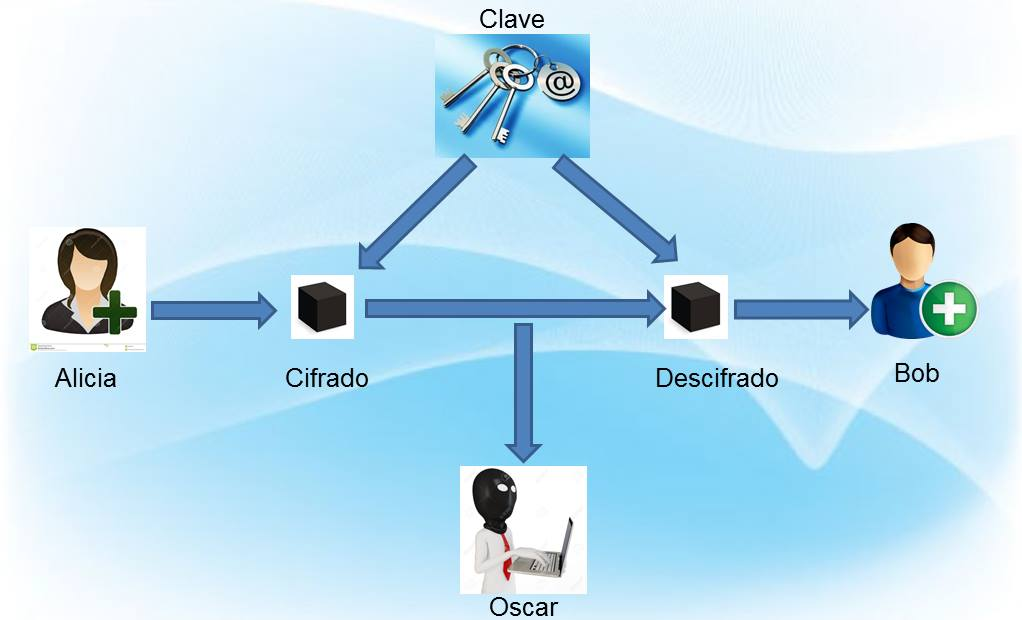
\includegraphics[width=10cm, height=5cm]{./images/simetrico.jpg}
	\caption{Diagrama cifrado simétrico}
	\label{fig:1-2-1}
\end{figure}

\subsection{Cifrado por bloques}
Este tipo de cifrado toma bloques de información del texto plano y produce bloques de información cifrados de un tamaño fijo, normalmente es del mismo tamaño que el bloque de información del texto plano. Los bloques de cifrado tienen que cumplir la condición de ser lo suficientemente grandes como para evitar ataques de texto cifrado, otra condición que se debe cumplir es que la asignación de bloques de entrada a bloques de salida es uno a uno para hacer el proceso reversible.\\
Formalmente un cifrado en bloque se considera que es seguro si se comporta como una permutación pseudoaleatoria fuerte, es decir, un cifrado de bloques es seguro si un adversario no puede distinguir su salida de una permutación elegida al azar.\\
Para hacer la asignación de bloques los algoritmos de cifrado utilizan sustituciones y permutaciones en los bloques de texto plano hasta obtener un texto cifrado.\\
La sustitución es el reemplazo de un bloque de $n$ bits por otro bloque de $n$ bits en un espacio de \(2^{k}\).\cite{bloc}\\
Los cifradores por bloques mas usados son:
\begin{itemize}
 \item Estandar de Cifrado de Datos DES (Data Encryption Standard)
 \item Estandar de cifrado Avanzado AES (Advanced Encryption Standard)
\end{itemize}


\subsection{Modos de operación}
Los modos de operacion fueron desarrollados para el algoritmo DES, estos fueron estandarizados en Diciembre de 1980. 
Cuando la informacion es cifrada usando la misma clave, surge una serie de problemas de seguridad. En esencia los modos de operacion son una técnica para mejorar el efecto criptografico de los cifradores por bloques.\cite{modes}\\\\
\textit{ECB}(Electronic codebook): Este modo de operación es probablemente el más simple de todos, el texto plano M está segmentado como $ M=M_1||M_2||...||M_m$ donde cada $M_i$ es un bloque de n bits. A continuación la funcion de cifrado $E_k$ se aplica por separado a cada bloque $M_i$. \\
A continuación tenemos el diagrama de este modo de cifrado.\\
\begin{figure}[h]
    \centering
    \begin{subfigure}[t]{0.5\textwidth}
        \centering
        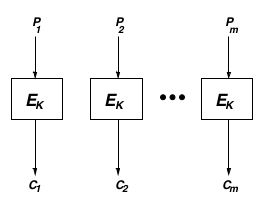
\includegraphics[height=1.7in]{./images/ecb1.png}
        \caption{Diagrama ECB Cifrado}
        \label{fig:1-3-1}
    \end{subfigure}%
    ~ 
    \begin{subfigure}[t]{0.5\textwidth}
        \centering
        \includegraphics[height=1.7in]{./images/ECB2.png}
        \caption{Diagrama ECB Descifrado}
        \label{fig:1-3-1}
    \end{subfigure}
    \label{fig:protocol}
\end{figure}


\textit{CBC}(Cipher-block chaining): Para este modo de operación la salida de un bloque de cifrado se introduce en el siguiente bloque de cifrado junto con el siguiente bloque del mensaje.\\

\begin{figure}[h]
    \centering
    \begin{subfigure}[t]{0.5\textwidth}
        \centering
        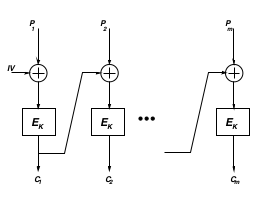
\includegraphics[height=1.7in]{./images/cbc1.png}
        \caption{Diagrama CBC Cifrado}
        \label{fig:1-4-1}
    \end{subfigure}%
    ~ 
    \begin{subfigure}[t]{0.5\textwidth}
        \centering
        \includegraphics[height=1.7in]{./images/CBC2.png}
        \caption{Diagrama CBC Descifrado}
        \label{fig:1-4-1}
    \end{subfigure}
    \label{fig:protocol}
\end{figure}

 \begin{figure}[H]
 \centering
	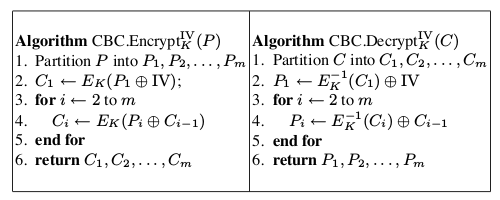
\includegraphics[width=14cm, height=6cm]{./images/pcbc.png}
	
\end{figure}

CBC toma como bloques de mensajes de entrada M y un vector de inicialización (IV). Durante el cifrado, la salida del i-ésimo bloque depende de los i-1 bloques anteriores. Así, el cifrado CBC es intrínsecamente secuencial.\\

\textit{CFB}(Cipher Feedback): En este modo de operación, los bloques de cifrado también están encadenados pero a la salida se produce de una manera muy diferente de la de CBC. Cada bloque de salida se le aplica XOR con el siguiente bloque de entrada.\\

\begin{figure}[h]
    \centering
    \begin{subfigure}[t]{0.5\textwidth}
        \centering
        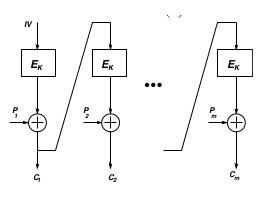
\includegraphics[height=1.7in]{./images/cfb1.png}
		\caption{Diagrama CFB Cifrado}
		\label{fig:1-5-1}
    \end{subfigure}%
    ~ 
    \begin{subfigure}[t]{0.5\textwidth}
        \centering
        \includegraphics[height=1.7in]{./images/CFB2.png}
		\caption{Diagrama CFB Descifrado}
		\label{fig:1-5-1}
    \end{subfigure}
    \label{fig:protocol}
\end{figure}

\begin{figure}[H]
\centering
	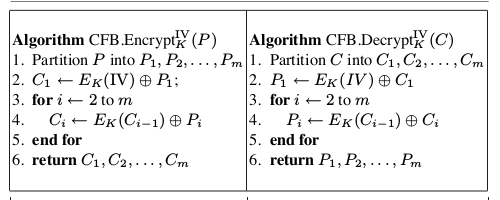
\includegraphics[width=14cm, height=6cm]{./images/pcfb.png}
	
\end{figure}


\textit{OFB}(Output feedback): En este modo de operación el IV se cifra varias veces para obtener un flujo de bytes aleatorios, el resultado de esto se aplica XOR con el bloque de texto plano mientras que el flujo de bytes aleatorios se usa como parámetro del siguiente bloque. A diferencia de los otros modos en OFB ninguna parte del texto claro entra directamente a cifrarse.

\begin{figure}[h]
    \centering
    \begin{subfigure}[t]{0.5\textwidth}
        \centering
        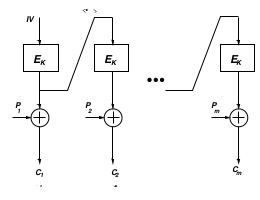
\includegraphics[height=1.7in]{./images/ofb1.png}
		\caption{Diagrama OFB Cifrado}
		\label{fig:1-6-1}
    \end{subfigure}%
    ~ 
    \begin{subfigure}[t]{0.5\textwidth}
        \centering
        \includegraphics[height=1.7in]{./images/OFB.png}
		\caption{Diagrama OFB Descifrado}
		\label{fig:1-6-1}
    \end{subfigure}
    \label{fig:protocol}
\end{figure}

\begin{figure}[H]
\centering
	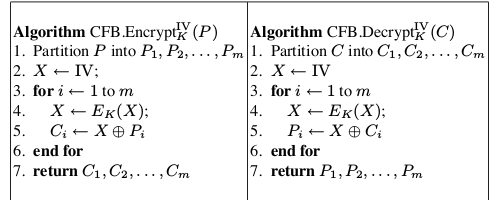
\includegraphics[width=14cm, height=6cm]{./images/pofb.png}
	
\end{figure}
\pagebreak
\section{Funciones Hash}
Las funciones hash son usadas pra construir una pequeña huella digital de la informacion, si la informacion es alterada tambien la huella digital es alterada. Esta caracteristica hace que las funciones hash sean ampliamente usadas para verificar la integridad de datos.\\
De manera formal, un funcion Hash es una Cuadrupla$(X,Y,K,H)$ donde:
\begin{enumerate}
 \item $X$ es un conjunto de posibles mensajes.
 \item $Y$ es un conjunto finito de posibles resúmenes de mensajes o etiquetas de autenticación.
 \item $K$, el espacio de claves, es un conjunto finito de posibles claves.
 \item Para cada $k\quad \epsilon\quad K$, existe una función hash $h_k\quad \epsilon\quad H$. Parac ada $h_k: X \longrightarrow Y$.
 \cite{stinson}
\end{enumerate}



\section{Aritmética Modular}
\textbf{Aritmética}:\\
En matemática, la aritmética modular es un sistema aritmético para clases de equivalencia de números enteros llamadas clases de congruencia.
La aritmética modular puede ser construida matemáticamente mediante la relación de congruencia entre enteros, que es compatible con las operaciones en el anillo de enteros: suma y multiplicación.
La aritmética modular se basa en una relación de equivalencia, y las clases de equivalencia de un entero a se denota con [a]n (o simplemente [a] si sobreentendemos el módulo.) $a\quad mod\quad n$. El conjunto de todas las clases de equivalencia se denota con $Zn = { [0]n, [1]n, [2]n,..., [n-1]n }.$
Un hecho importante sobre aritmética modular, cuando los módulos son números primos es el pequeño teorema de Fermat: si p es un número primo, entonces.\cite{modular}\\\\
Si $a$ es cualquier entero:\\\\
$a^p\equiv a(mod\quad p)$\\\\
Si $a$ es un entero no divisible entre $p$:\\\\
$a^{p-1}\equiv 1(mod\quad p)$\\\\
\textbf{Numeros primos}:\\
Los números primos son aquellos números enteros que sólo son divisibles por si mismos y por la unidad. Los numeros que no son primos se llaman compuestos, excepto el numero 1 que no se considera ni primo ni compuesto. En el libro IX Euclides demostró que existe una infinidad de numeros primos.\\\\
\textbf{Anillo}: Un anillo es un sistema algebraico formado por un conjunto no vacío y dos operaciones internas, llamadas usualmente suma y producto. El producto en un anillo no necesariamente tiene una operación inversa definida, aun que puede ser definida por su inverso multiplicativo.\cite{anil}\\\\ 
\\
\textbf{Zp}:\\
Sea $Zp$ un conjunto de elementos con dos operaciones binarias, suma y multiplicación y $p$ sea un numero primo. Dicho conjunto tendra estructura de anillo si satisface.\cite{zp}
\begin{itemize}
 \item $Zp$ es asociativa bajo la multiplicación.\\\\
 $(a . b) . c  =  a . (b . c)$
 \item La multiplicación es distributiva respecto a la suma.\\
 Para $a,b,c\quad\epsilon\quad Zp$\\\\
 $a.(b+c)=a.b+a.c$\\\\
 $(a+b).c=a.c+b.c$
\end{itemize}


\textbf{Euclides Extendido}:\\
Una de las técnicas básicas de la téoria de números es el algoritmo de Euclides, que es un procedimiento simple para la determinación del maximo comun 	divisor de dos números enteros positivos.\\
$b$ se define como un divisor de $a$ si $a=mb$ para algun $m$ tal que $a$,$b$ y $m$ son numeros enteros.
Utilizaremos la notación $gcd (a, b)$ que significa el máximo común divisor de a y b.\\
Supongamos que tenemos los numeros enteros $a$, $b$ de tal manera que $d=gcd(a,b)$, suponiendo que $a\geq b > 0$. Ahora dividir $a$ entre $b$ y aplicando el algoritmo de la división:\\\\
$a=q_1b++r_1$   donde $0\leq r_1<0$.\\\\
Sucede que si $r_1=0$ entonces $gcd(a,b)=b$ pero si $r_1\neq 0$. Se procede a resolver $gcd(b,r_1)$ y se aplica el algoritmo de divicion.\\\\
$b=q_2r_1+r_2$\\\\
Del mismo modo si $r_2=0$ entonces $gcd(b,r_1)=r_1$ y si $r_2\neq 0$, entonces continua el proceso de divicion con $gcd(r_1,r_2)$. El resultado es el siguiente sistema de ecuaciones:\\\\
$a=q_1b+r_1$\\
$b=q_2r_1+r_2$\\
$r_1=q_3r_2+r_3$\\
$.$\\
$.$\\
$.$\\
$r_{n-2}=q_nr_{n-1}+r_n$\\
$r_{n-1}=q_{n+1}r_n+0$\\
$gcd(a,b)=r_n$\\\\
Para los enteros $a$, $b$ el algoritmo de Euclides Extendido no solo calcula el maximo comun divisor $d$ si no que adicionalmente se calculan los numeros $x$, $y$ tal que.\\\\
$ax+by=d=gcd(a,b)$\\
Con base en esto el calculo del algoritmo de euclides extendido para $(x,y,d)$. Dado  $a$ y $b$ usamos la secuencia de diviciones indicada en las ecuaciones anteriores, y suponemos que en cada paso podemos encontrar $i$ enteros $x_i$ y $y_i$ que satisfagan la ecuacion $r_i=ax_i+by_i$.\\
Tenemos la secuencia:\\
$a=q_1b+r_1$\\
$b=q_2r_1+r_2$\\
$r_1=q_3r_2+r_3$\\
$.$\\
$.$\\
$.$\\
$r_{n-2}=q_nr_{n-1}+r_n$\\
$r_{n-1}=q_{n+1}r_n+0$\\\\
De esta secuencia podemos reordenar los terminos de la forma:\\
$r_n=r_{n-2}-r_{i-1}q_i$ ... (1.1)\\
Además, en filas $i-1$ e $i-2$ nos encontramos con los valores:\\
$r_{i-2}=ax_{i-2}+by_{i-2}$ y $r_{i-1}=ax_{i-1}+by_{i-1}$\\
Y sustituimos estas en la ecuacion (1.1) quedando.\\
$r_i=a(x_{i-2}-q_ix_{i-1})+b(y_{i-2}-q_iy_{i-1})$
\cite{modes}\\

\section{Polinomio de Lagrange}
 El polinomio de Lagrange, llamado así en honor a Joseph-Louis de Lagrange, es una forma de presentar el polinomio que interpola un conjunto de puntos dado. Este genera una aproximacion a una funcion dependiendo de los puntos que se introduscan.\cite{stinson}\\\\
 
 Dado un conjunto de $k + 1$ puntos\\\\
 $(x_0,y_0),...,(x_k,y_k)$\\\\
 donde todos los $x_j$ se asumen distintos, el polinomio interpolador en la forma de Lagrange es la combinación lineal.
 \begin{equation}
  L(x)=\sum_{j=0}^{k}y_jl_j(x)
 \end{equation}
 \\\\
 de bases polinómicas de Lagrange\\\\
 \begin{equation}
  l_j=\prod_{i=0,i\neq j}^{k}\frac{x-x_i}{x_j-x_i}=\frac{x-x_0}{x_j-x_0}...\frac{x-x_{j-1}}{x_j-x_{j-1}}\frac{x-x_{j+1}}{x_j-x_{j+1}}...\frac{x-x_k}{x_j-x_k}
 \end{equation}
El uso del Polinomio de Lagrange nos permite calcular de manera mas rapida un sistema de ecuaciones de la forma $a_0+a_1.x^1+...+a_n.x^n$.

%\chapter{Adversarios Clasificadores}

En este capitulo hablaremos de los adversarios clasificadores, los algoritmos y algunas herramientas que se han desarrollado para proteger al correo electrónico contra estos adversario.

\section{Adversarios}

Los adversario clasificadores son programas que se dedican a observar los mensajes que se intercambian  entre  los  usuarios  de  correo  electrónico,  con  el  fin  de  clasificarlos  e 
identificar  a  todos  los  usuarios  que  cumplan  con  cierto  criterio.  Esta  clasificación  se hace de manera masiva y la realiza haciendo una búsqueda de palabras clave dentro de 
los  mensajes de  los usuarios. Por ejemplo, el  clasificador puede estar interesado en  los mensajes  que  contienen  la  palabra  clave  "Bomba",  así  que 
todos  los  mensajes  que contengan esta palabra serán etiquetados en una clasificación en específico, este proceso se lleva a cabo por medio de técnicas de 
“Reconocimiento de patrones” y “Aprendizaje Máquina” para encontrar y clasificar los mensajes que intercepta.\cite{clas,Attacks}
\\
La  clasificación  de  estos  mensajes  tiene  diversos  usos, ya  que  pueden  ser  clasificados con  fines demográficos, con  fines comerciales o con  fines gubernamentales. Todo esto 
con  el  propósito  de  generar  las  estadísticas  de  comportamientos  e  intereses  de  los usuarios de correo electrónico. \\




En este trabajo terminal, se considera el tipo de ataque llamado “ataque  de  texto  cifrado” o COA  que  hace  referencia  a  su  nombre  en  inglés “
Ciphertext-only  attack”\cite{Ciphertextonly}.  Este ataque  solo  cuenta  con  los  textos  cifrados  que  va  recopilando  de  un  canal  o  base  de 
datos,  estos  textos  cifrados  los  utiliza  para  hacer  un  análisis  criptográfico  de  cómo  se comporta la técnica de cifrado  y trata de hallar el texto en claro a partir de los textos cifrados que va recopilando. 
\\
Este  tipo  de  ataques  es  muy  común  en  el  internet  aunque  con  muy  baja  efectividad cuando   se   implementa   en   comunicaciones   altamente   protegidas,   y   cuando   se 
implementa en canales de comunicación desprotegidos  la  información obtenida  llega  a ser  muy  pobre.  En  los  últimos  años  se  han  dado  cuenta  que  si   este  tipo  de 
adversarios   atacan las  comunicaciones  sin  cifrado se  obtienen  características  valiosas  sobre  los usuarios  que  utilizan  este  tipo  de  canales  de  comunicación,  este  tipo  de  ataques  son 
ejecutados por  adversarios clasificadores.\\


\subsection{Esquema Golle - Farahat}
La  única  referencia  que se tiene  sobre  un  esquema  criptográfico  contra  adversarios clasificadores es el que encontramos en el artículo 
“Defending Email Communication Against Profiling” de Philippe Golle  y  Ayman  Farahat, ambos  miembros del 
“Palo Alto Research Center”.\cite{Attacks}\\
En su artículo se aborda el ataque de adversarios clasificadores sobre los mensajes de correo electrónico, en el cual se proponen un protocolo para la comunicación por correo electrónico. Este protocolo hace uso de una función  de cifrado que sustituye cada una de las palabras del mensaje por otra de la misma extensión y frecuencia gramatical, esta función esta pensada para textos en idioma ingl\'es. 
Esta función tiene como parámetro una clave $K$.  Para calcular esta clave se usan los datos de cabecera que acompañan al mensaje los cuales pueden ser dirección  del remitente, la dirección del destinatario, la hora a la que se envía el correo electrónico y potencialmente otros campos. Estos datos se introducen en una función hash lenta y el resultado de esta función es la clave $K$. Estas funciones hash  tiene con una complejidad de calculo moderadamente mas alta.  \\
Este  protocolo resulta inseguro para la criptografía clásica pero es efectivo contra el ataque de clasificadores. Por otro lado este protocolo resuelve dos problemas, le  permite  a los usuarios  calcular  la  clave de cifrado y descifrado  fácilmente  ya  que  los datos del mensaje con que se calcula son  públicos, resolviendo así el intercambio de claves. Al usar un cifrado de tipo semántico se permite que el texto se vea como un texto en inglés pero indistinguible para los clasificadores y por lo tanto este clasifica incorrectamente el mensaje cifrado.\\

\section{CAPTCHA}
 Es un programa informático diseñado para diferenciar un ser humano de una computadora, CAPTCHA son las siglas de prueba de Turing completamente automática y pública para diferenciar computadoras de humanos (Completely Automated Public Turing test to tell Computers and Humans Apart).  Un CAPTCHA es una prueba que es fácil de pasar por un usuario humano pero difícil de pasar por una máquina. Uno de los CAPTCHAs más com\'unes son imágenes distorsionadas de cadenas cortas de caracteres. Para un humano es generalmente muy fácil recuperar la cadena original de la imagen distorsionada, pero es difícil para  los algoritmos de reconocimiento de caracteres recuperar la cadena original de la imagen distorsionada.\\
Un CAPTCHA en un algoritmo aleatorio $G$, que recibe como parámetro una cadena de caracteres STR y produce como resultado un CAPTCHA $G(x)$\\

\begin{figure}[H]
\centering
	
\includegraphics[width=5cm, height=3cm]{./images/cptc.jpeg}
	\caption{CAPTCHA}
	\label{fig:3-6}
\end{figure}
 
%La criptografía moderna se basa en dos corrientes metodológicas que son la criptografía simétrica  y  la criptografía asimétrica. Estas dos técnicas tienen como propósito ocultar 
%el  contenido  de  un  mensaje  con  el  fin  de  que  solo  sea  leído  por  aquellos  que  estén autorizados, a esto se le llama cifrado. 




\section{Esquema de Secreto Compartido de Shamir}
El secreto compartido, es un método dise\~nado para compartir un objeto entre un grupo de participantes. Este método fue propuesto por Adi Shamir en 1997.\cite{shamir}
\\
\\
El objetivo de este método es dividir un secreto $K$ en $w$ partes,que son dadas a $w$ participantes. Para recuperar el secreto es necesario tener al menos $u$
elementos de las $w$ partes siendo $u \leq w$. Y no es posible recuperar el secreto si se tienen menos que $u$ partes.
\\
\\
Para construir el esquema del secreto compartido primero es necesario seleccionar un número primo $p \geq w+1$ el cual define el anillo $Z_p$.
\\
\\
El procedimiento para dividir un secreto $K$ en $w$ partes es el siguiente:

\begin{enumerate}
 \item Se seleccionan $w$ elementos distintos de cero del anillo $Z_p$ denotados como $x_i$ donde $1 \leq i \leq w$.
 \item Se seleccionan $u-1$ elementos aleatorios de $Z_p$ denotados como $a_1,...,a_{u-1}$.
 \item Se construye el polinomio $y_x$ de la siguiente forma. Sea \begin{equation}
            y(x)=K+\sum_{j=1}^{u-1} a_j x^j mod \quad p
           \end{equation}
           Por medio de este polinomio se calculan los elementos $y_i$.
 \item La salida es el conjunto $S=\{(x_1,y_1),...,(x_w,y_w)\}$.
\end{enumerate}

Para recuperar el secreto solo tenemos que resolver un sistema de ecuaciones que es definido por el polinomio característico $a(x)=a_0+a_1x+...+a_{u-1}x^{u-1}$.
\\
\\
Posteriormente se seleccionan $u$ pares de elementos $(x_w,y_w)$ con los que obtendremos nuestro sistema de ecuaciones a resolver. El elemento que nos interesa obtener del sistema de ecuaciones es $a_0$ ya que este es el valor de nuestro secreto $K$.
\\
\textbf{Ejemplo}
Se selccion\'o un anillo  $Z_p=11$\hspace{0,4cm} con \hspace{0,4cm}$w=5$\hspace{0,4cm} incógnitas de las que se resuelven\hspace{0,4cm}$u=2$.\hspace{0,4cm}Se seleccion\'o como llave\hspace{0,4cm}$k=8$\hspace{1cm}
\\ 
\\
Se selecciona los $u-1$ elementos del anillo $Z_p$\\
$a_1=5$ 
\\
\\
Del anillo $Z_p$ se seleccionan los $w$ elementos $x_i$\\
$x_1=2$\hspace{1cm}$x_2=7$\hspace{1cm}$x_3=9$\hspace{1cm}$x_4=10$\hspace{1cm}$x_5=3$\\
\\
Se calcula el conjunto de elementos $y_i$ por medio de la ecuaci\'on 
\begin{equation}
 y_i=k+\sum_{j=1}^{u-1} a_j x_i^j mod \quad p
\end{equation}
\\
Sustituyendo la sumatoria para nuestro caso queda
\\
\begin{equation}
 y_i=K+a_1x_i^1mod \quad p
\end{equation}
\\
$y_1=8+5(2)mod11=7$\hspace{3,5cm}$y_2=8+5(7)mod11=10$\hspace{3,5cm}$y_3=8+5(9)mod11=9$\hspace{3,5cm}$y_4=8+5(10)mod11=3$\hspace{3,5cm}$y_5=8+5(3)mod11=1$\\
\\
Se tienen los pares $S=(A_n(x_n,y_n))$\\
$A_1(2,7)$\hspace{1cm}$A_2(7,10)$\hspace{1cm}$A_3(9,9)$\hspace{1cm}$A_4(10,3)$\hspace{1cm}$A_5(3,1)$\\
\\
Para recuperar la llave $K$ es necesario seleccionar $u$ pares del conjunto $S$, los seleccionados son:\\
$A_2(7,10)$\hspace{1cm}$A_4(10,3)$\\
\\
Con estos pares podemos calcular un sistema de ecuaciones resolviendo el polinomio característico para $u=2$\\
$a_0+a_1x=y$ donde $a_0=k$\\
De lo que resulta el siguiente sistema de ecuaciones al sustituir los pares $A_2$ y $A_4$ en el polinomio\\
$a_0+7a_1=10$\\
$a_0+10a_1=3$\\
\\
Para resolver este polinomio podemos utilizar cualquiera de los métodos comunes que se usan en álgebra, solo que respetando el anillo $Z_p$, en este caso se resolverá por el método suma y resta.\\
\\
\begin{equation}
 a_0+7a_1=10
\end{equation}
\begin{equation}
 a_0+10a_1=3
\end{equation}
Multiplicamos la ecuación (3) por $-1$ y obtenemos el siguiente sistema:
\begin{equation}
 -a_0-7a_1=-10
\end{equation}
\begin{equation}
 a_0+10a_1=3
\end{equation}
sumamos la ecuación (5) + (6) dandonos como resultado:
\begin{equation}
 3a_1=4
\end{equation}
De la ecuación (7) despejamos $a_1$
\begin{equation}
 a_1=\frac{4}{3}
\end{equation}
Siendo 4 el inverso multiplicativo de 3 la ecuación (8) queda de la siguiente forma
\begin{equation}
 a_1=(4)(4)=16 mod11 =5
\end{equation}
Sustituimos $a_1$ en la ecuación (4) 
\begin{equation}
 a_0+10(5)=3
\end{equation}
Simplificamos y despejamos $a_0$
\begin{equation}
 a_0+(50mod11)=3
\end{equation}
\begin{equation}
 a_0+6=3
\end{equation}
\begin{equation}
 a_0=3-6
\end{equation}
\begin{equation}
 a_0=-3mod11=8
\end{equation}

Como $a_0=8$ podemos ver que esto es verdad por que $a_0=K$ y el $K$ que seleccionamos es $K=8$ con lo que recuperamos $K$ exitosamente.


\section{Codificaci\'on de caracteres a enteros}
Se tiene un conjunto de caracteres $AL$ compuesto por $AL=\{A,B,...,Z\}\cup\{a,b,...,z\}\cup\{0,1,...,9\}\cup\{+,/\}$ con una cardinalidad $|AL|=64$.

Para obtener una representación binaria de 64 elementos son necesarios 6 bits por lo que para todos los elementos $\sigma\epsilon AL$ existe una cadena binaria. Una vez establecido esto el procedimiento para realizar la conversión es el siguiente:
\begin{enumerate}
 \item Tomamos una cadena de caracteres y la separamos caracter por caracter y los intercambiamos por su correspondiente número entero en $AL$ $\alpha _0||\alpha _1||...||\alpha _m$
 \item Posteriormente cada uno de los enteros lo convertimos en un binario de 6 bits y se concatenan uno detrás del otro $\Psi\longleftarrow bin_6(\alpha _0)||bin_6(\alpha _1)||...||bin_6(\alpha _m$
 \item La cadena binaria $\Psi$ la convertimos a entero $v\longleftarrow toInt(\Psi)$
\end{enumerate}
\textbf{Ejemplo}:\\
Tenemos la cadena $STR=`ABC`$ de la cual cambiaremos cada caracter por su correspondiente valor entero en $AL$ quedando de la siguiente manera $\alpha =\{0,1,2\}$
\\ 
\\
Ahora cada  uno de los elementos de $\alpha$ lo convertiremos a su correspondiente representacion binaria, $bin_6(0)=000000, bin_6(1)=000001, bin_6(2)=000010$ y concatenamos cada una quedando $\Psi = 000000000001000010$. 


La cadena binaria $\Psi$ se convertirá en un entero $v=toInt(\Psi )$ que da como resultado $v=66$. El entero $v$ que obtenemos es el valor entero.

\section{Decodificación de enteros a caracteres}

También es necesario convertir un entero a una cadena de caracteres y para esto se realiza el proceso inverso:
\begin{enumerate}
 \item El entero $v$ es convertido en un número binario  $z=toBin_6(v)$ 
 \item Separamos $z$ en cadenas de 6 bits y cada una de ellas la interpretamos como un entero $toInt(z_0)||toInt(z_1)||...||toInt(z_w)$
 \item Cada uno de estos valores se convierte a su correspondiente caracter en $AL$ se concatenan para generar la cadena de caracteres final.
\end{enumerate}
\textbf{Ejemplo}:\\
El entero $v=66$ se representa como una cadena de 18 bits $z=000000000001000010$, la cual se divide en sub cadenas 6 bits quedando $z_0=000000, z_1=000001, z_2=000010$, para cada uno de estos números binarios se procede a convertirlo en un entero $toInt(z_0)=0, toInt(z_1)=1, toInt(z_2)=2$, por último estos son intercambiados por sus correspondientes caracteres en $AL$ y concatenados resultando en $s=`ABC`$


\subsection{Esquema Díaz - Chakraborty}
El esquema propuesto en el articulo ``On Securing Communication from Profilers.'' de Sandra Díaz Santiago y Debrup Chakraborty.\cite{clas}\\\\
Al igual que en el Esquema Golle - Farahat en este articulo se aborda el ataque de adversarios clasificadores sobre el correo electrónico, solo que en este se proponen dos esquemas para resolver este problema.
\begin{enumerate}
 \item \textbf{Esquema P}: Se genera una cadena de caracteres aleatoriamente llamada STR la cual es introducida a una funcion Hash para generar la clave $K$, con esta clave se cifra el mensaje original $M$. La cadena STR es convertida en un CAPTCHA y se envía junto con el texto cifrado al destinatario.\\\\
 \textbf{Esquema} P(x)
 \begin{enumerate}
  \item $k\longleftarrow^\$ STR;$
  \item $k'\longleftarrow G(k);$
  \item $K\longleftarrow H(k);$
  \item $c\longleftarrow E_k(x);$
  \item $return(c,k')$
 \end{enumerate}
 Contemplando que es muy común que el usuario no consiga resolver el CAPTCHA se pensó en el siguiente esquema.
 \item \textbf{Esquema P'}: Se genera una cadena de caracteres aleatoriamente llamada STR la cual se codifica a un valor entero. El valor entero es dividido en 5 pares $(x,k')$ por medio del algoritmo de Secreto Compartido, cada uno de los elementos $k'$ de los pares generados es decodificado a su correspondiente valor en cadena de caracteres para posteriormente ser convertidos en CAPTCHAS. Para finalizar la cadena STR se introduce en una función Hash para generar la llave $K$. Con esta llave se cifra el mensaje de correo y se envía junto con los pares de $(x,CAPTCHA)$.
 \begin{enumerate}
  \item $k\longleftarrow^\$STR;$
  \item $k'\longleftarrow ENCD(k);$
  \item $\{(x_1,k'_1),...,(x_w,k'_w)\}\longleftarrow SHARE^p_{u,w}(k');$
  \item $for\quad i=1\quad to \quad w;$
  \item $\quad (k_i)\longleftarrow ENCD^{-1}(k'_1);$
  \item $\quad c_i\longleftarrow G(k_i);$
  \item $end for$
  \item $K\longleftarrow H(k);$
  \item $C\longleftarrow E_k(x);$
  \item $return [C,\{(x_1,c_1),...,(x_w,c_w)\}]$
 \end{enumerate}

\end{enumerate}
Este nuevo esquema se creo pensando en que el usuario pueda tener más oportunidades de recuperar el mensaje cifrado y esto sucede gracias a el algoritmo de Secreto Compartido, ya que no este podemos tener la misma llave repartida en $n$ CAPTCHAS.


        

%\chapter{Tecnologías usadas}

Tomando en cuenta la información ya vertida en este documento, a continuación se explicará detalladamente la propuesta de solución.\\
En la figura \ref{fig:4-1-1} se tiene el diagrama general del sistema, se puede apreciar la comunicación entre las diferentes entidades que se usaran, que datos se mandan y reciben y por que canales transitan estos datos. A continuación se describe de manera general como es el proceso de envío y recepción de correos electrónicos ideado para este esquema.\\
\begin{enumerate}
 \item {Envío}
\begin{itemize}
\item El remitente escribe el correo electrónico y le da enviar.\\
\item El correo electrónico pasa por el complemento del cliente de correo.\\
\item El cliente genera a partir del correo una clave que usaremos para cifrar el mensaje.\\
\item Se cifra y se empaqueta el mensaje con el protocolo SMTP.\\
\item Se coloca una bandera en el mensaje.\\
\item La clave se convierte en CAPTCHA y es enviada al servidor de CAPTCHAS.\\
\item Se envía el mensaje de correo electrónico al destinatario.\\
\end{itemize}

\item{Recepción}
\begin{itemize}
\item El receptor abre un correo electrónico cifrado con el presente esquema.\\
\item El cliente lo descarga del servidor por medio del protocolo POP3 o IMAP.\\
\item Se hace una petición al servidor de CAPTCHAS para recuperar los CAPTCHAS del correo.\\
\item El usuario resuelve el CAPTCHA y se recalcula la clave de descifrado.\\
\item Se descifra el mensaje y se le muestra al usuario.\\
\end{itemize}
\end{enumerate}
\begin{figure}[h]
	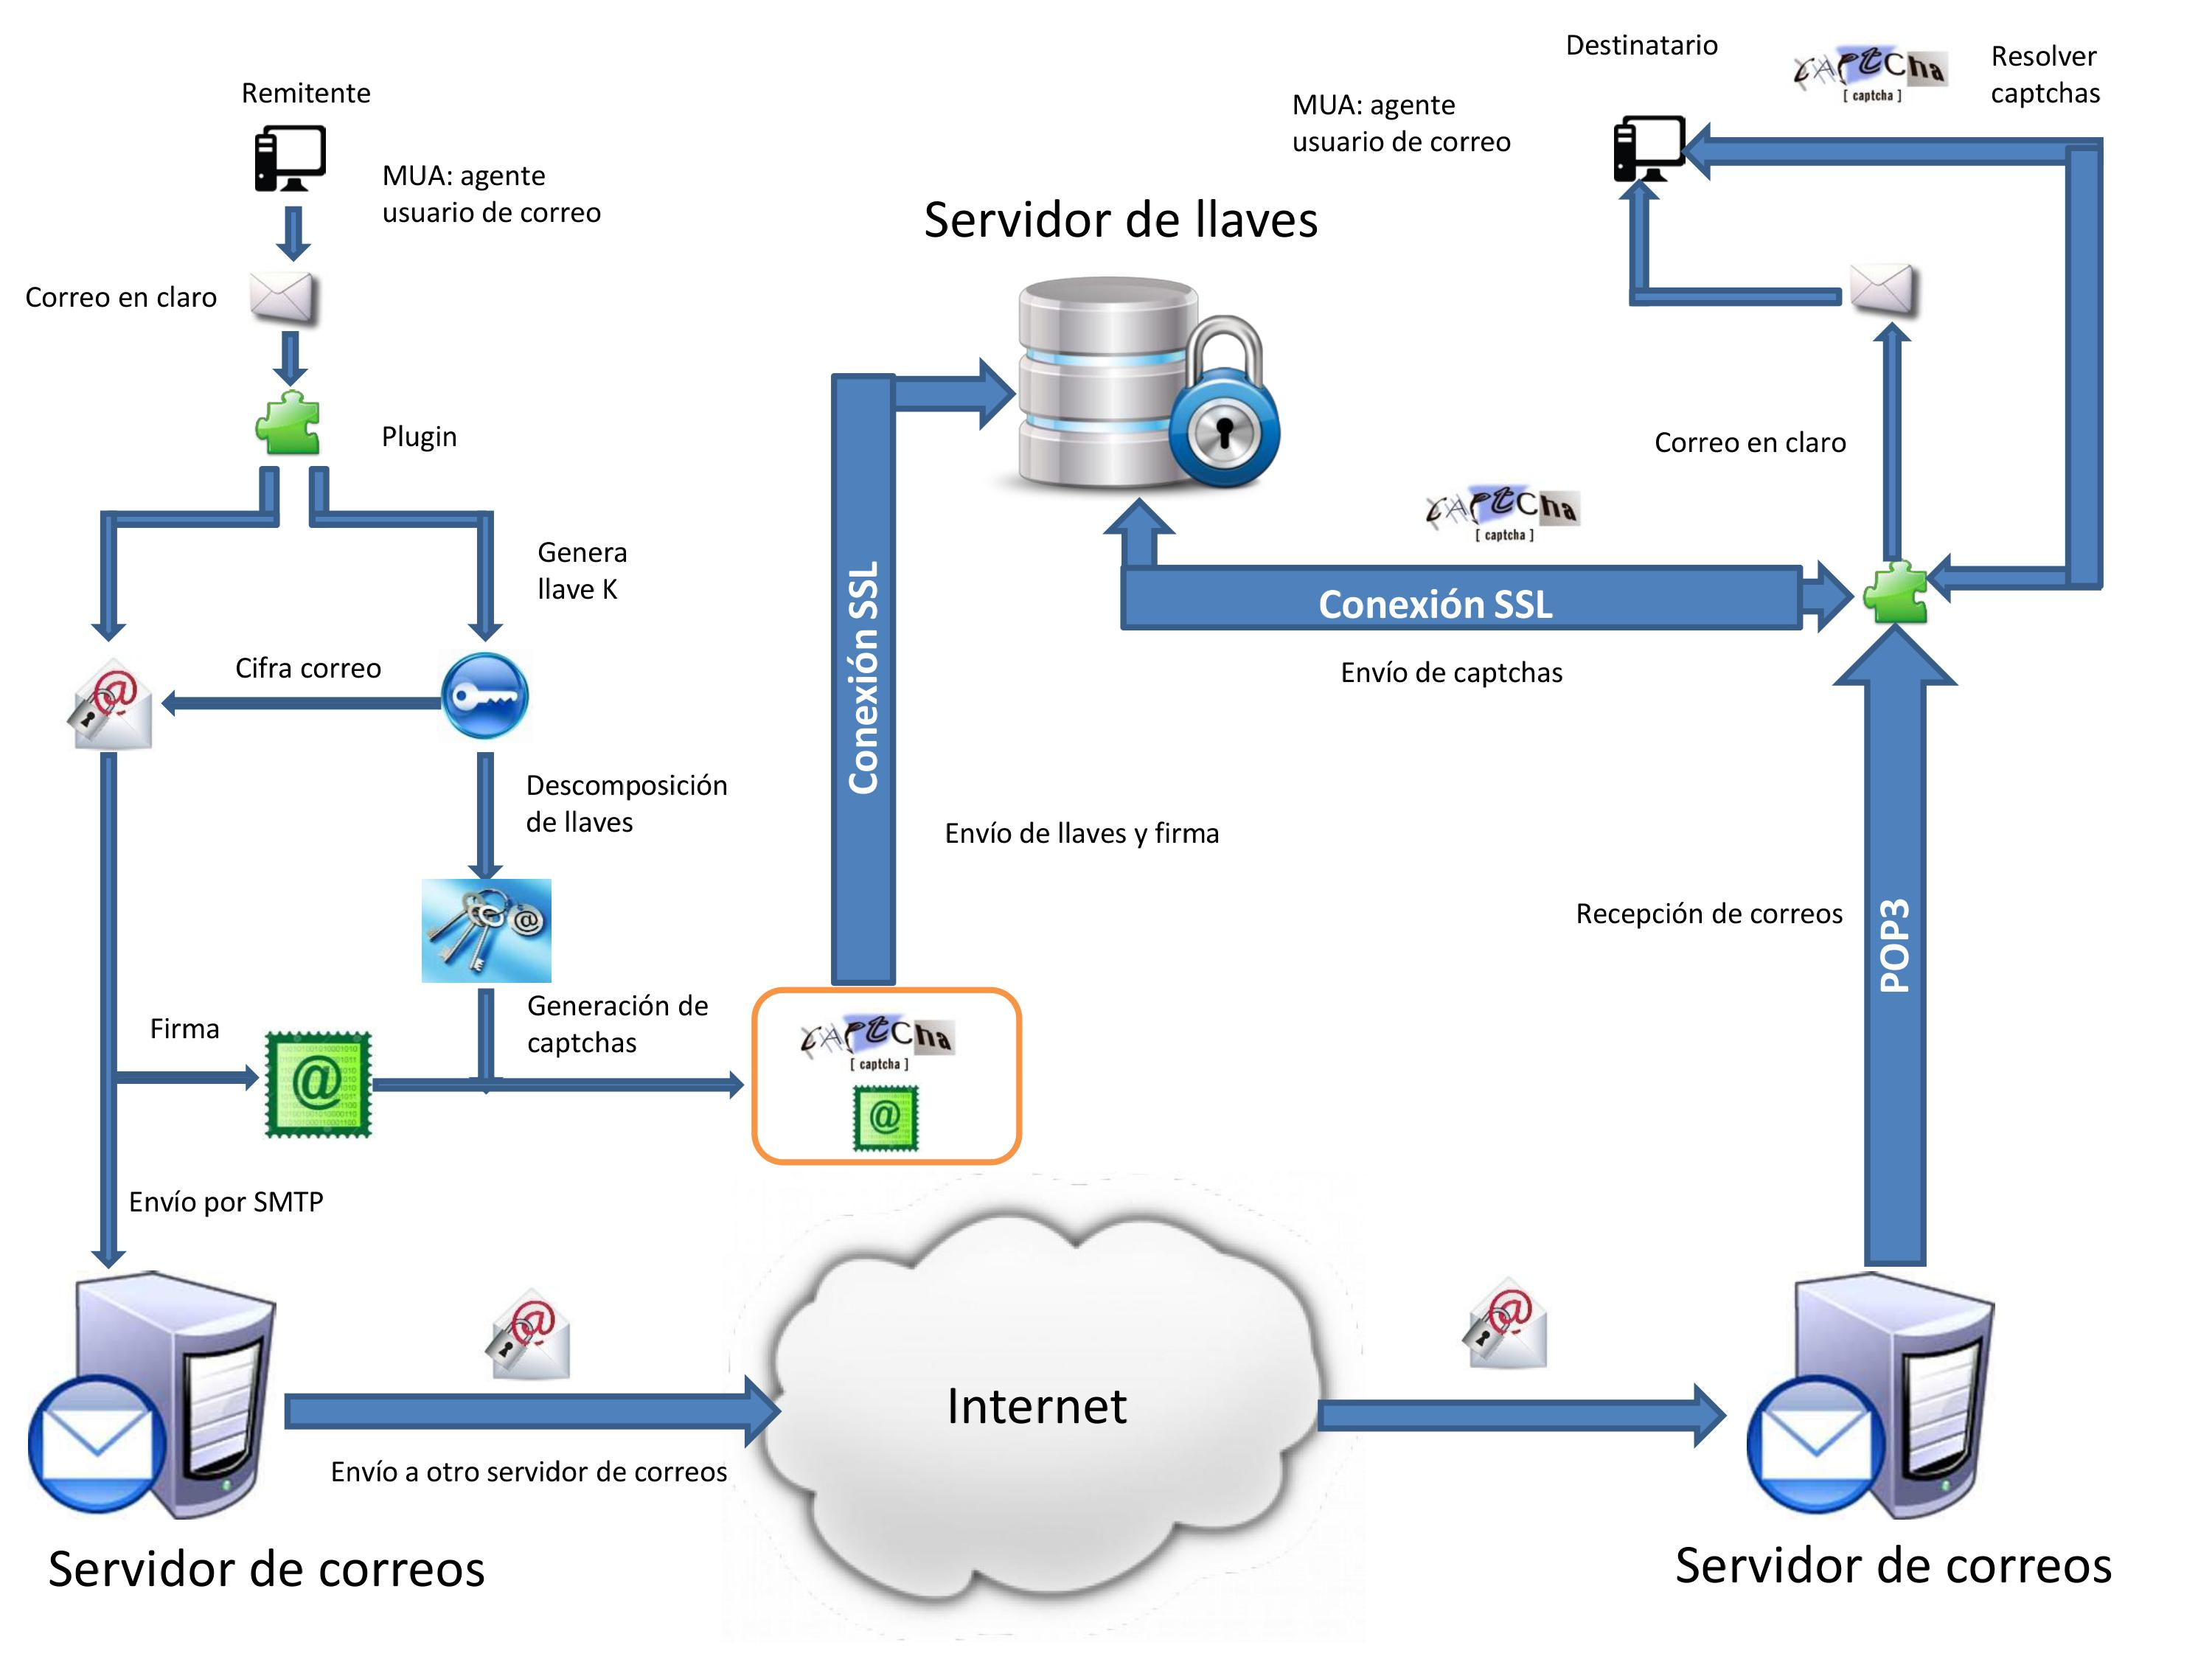
\includegraphics[width=1\linewidth, height=10cm]{./images/0001.jpg}
	\caption{Diagrama General del sistema}
	\label{fig:4-1-1}
\end{figure}
\section{Tecnologías}
Como ya se ha visto en el esquema anterior se necesita hacer uso de las herramientas adecuadas para poder desarrollar este esquema de cifrado. Las herramientas que se analizaron se describen en las siguientes secciones.\\
\subsection{Cliente de correo electrónico}
Un cliente de correo electrónico es necesario para el desarrollo de este proyecto ya que en él se instalará un complemento que cifre el mensaje, envíe los CAPTCHAS y descifre los mensajes de correo electrónico. Para ello buscamos un cliente de correo electrónico que cuente con el soporte de los protocolos POP3, SMTP y IMAP; sus licencias son de código libre; soporte la instalación de APIs externas; y tenga soporte en los sistemas operativos \textbf{\textit{Windows}}, \textbf{\textit{IOS}} y \textbf{\textit{Linux}}. Por lo tanto se investigaron los siguientes clientes de correo electrónico que se encuentra en el mercado: \\
\begin{longtable}[H]{| p{2,5cm} | p{2cm} |p{2cm}|p{1,5cm}|p{2cm}|p{3cm}|p{2cm}|}%\footnotesize
 \hline
 \textbf{Cliente de correo electrónico}&\textbf{Sistema Operativo}&\textbf{Protocolos soportados}&\textbf{Código Libre}&\textbf{Agregar funcionalidad}&\textbf{Extra}&\textbf{Gratuita o de paga}\\
 \hline
 \textbf{eM client}&Windows 7, 8 \& 10 ; IOS&POP3, SMTP, IMAP, EWS, AirSyn&NO&NO&100\% compatible con gmail y sus APIs&Ambos\\
 \hline
 \textbf{Postbox}&Windows, IOS&POP3, SMTP, IMAP&NO&SI por medio de APIs&Sincronización con Dropbox, OneDrive, Facebook y Twitter&Ambos\\
 \hline
 \textbf{Zimbra}&Windows, IOS \& Linux&POP3, SMTP, IMAP&SI&SI por medio de APIs&Una plataforma de nivel empresarial y capas se soportar sincronización con múltiples servicios&Ambos\\
 \hline
 \textbf{Opera Mail}&Windows, IOS \& Linux&POP3, SMTP, IMAP&SI&NO&La plataforma para desarrollar en Opera se actualiza cada semana&Gratuito\\
 \hline
 \textbf{Thunderbird}&Windows, IOS \& Linux&POP3, SMTP, IMAP&SI&SI por medio de APIs&Cliente de correo versátil y fácilmente escalable y una comunicad de desarrollo bastante amplia&Gratuito\\
 \hline
 \textbf{Nylas N1}&Windows, IOS \& Linux&POP3, SMTP, IMAP&SI&Si directamente compilando& &Gratuito
 
    \label{tabla:Descripcion de clientes}
    \\
  \hline

\end{longtable}

\begin{itemize}
 \item El cliente de correo electrónico \textbf{\textit{eM client}} tiene una sincronización a 100\% con las cuentas de \textbf{\textit{Gmail}} y sus APIs, cuenta con una versión gratuita y una versión de paga; puede hacer migración de mensajes de correo electrónico y contactos de diversos clientes de correo electrónico y tiene una compatibilidad con muchos servidores de correo electrónico.\cite{em}\\Su desventaja es que su código es cerrado y permite agregar funcionalidades.
 \item El cliente de correo electrónico \textbf{\textit{Postbox}} esta soportada en los sistemas operativos \textbf{\textit{Windows 7}} o posteriores y \textbf{\textit{IOS}}, esta aplicación es generada por el servidor de correo electrónico \textbf{\textit{Postbox}} por lo tanto cuenta con una sincronización al 100\% con este servidor, también soporta otros servidores de correo como \textbf{\textit{Gmail}} y \textbf{\textit{Outlook}}; este cliente puede sincronizarse con \textbf{\textit{Dropbox}}, \textbf{\textit{Onedrive}} y redes sociales como \textbf{\textit{Facebook}}, \textbf{\textit{Twitter}}, entre otras. Es posible agregar más funcionalidades con la instalación de APIs.\\Una desventaja de esta aplicación es que su código es cerrado, pero gracias a que esta basado en código de \textbf{\textit{Mozilla}} puedes desarrollar APIs para agregarle tus propias funciones. \cite{box}
 \item El cliente de correo electrónico \textbf{\textit{zimbra}} es la aplicación más completa que se analizó, tiene compatibilidad con el servidor \textbf{\textit{zimbra}} pero es capaz de soportar otros servidores de correo electrónico, se encuentra en los 3 sistemas para PC, \textbf{\textit{Windows}}, \textbf{\textit{IOS}} \& \textbf{\textit{Linux}}, da la facilidad de agregarle funcionalidades por medio de la instalación de APIs y gracias a que su código es abierto se pueden programar funciones propias. Este cliente cuenta con la versión gratuita y la versión de paga. Una gran ventaja que tiene es que oferta certificaciones en el desarrollo APIs para este cliente de correo electrónico.\cite{zim}\\La única desventaja que se encontró en este cliente de correo es que la plataforma es demasiado grande y el tiempo que se necesita invertir al estudio del código es demasiado y el tiempo de desarrollo de este proyecto es muy corto.
 \item \textbf{\textit{Opera mail}} es un cliente de correo electrónico que salió al mercado recientemente y se puede instalar en los sistemas operativos \textbf{\textit{Windows}}, \textbf{\textit{IOS}} \& \textbf{\textit{Linux}}, es capaz de comunicarse con diversos servidores de correo electrónico y su código es de libre acceso.\\Su principal desventaja es que las funcionalidades que se quieran agregar no pueden ser adquiridas por medio de la instalación de complementos o APIs.\cite{opera}
 \item Por último tenemos a \textbf{\textit{Thunderbird}} que es un cliente de correo electrónico desarrollado por \textbf{\textit{Mozilla}}, este cliente es de código abierto y la instalación de APIs para agregar funcionalidad es demasiado sencilla; es un cliente de correo que puede ser instalado en los sistemas operativos \textbf{\textit{Windows}}, \textbf{\textit{IOS}} y \textbf{\textit{Linux}}.\cite{thun}
\end{itemize}
Por lo tanto el cliente de correo electrónico que se usará es \textbf{\textit{Thunderbird}}, al ser un cliente de correo electrónico casi tan completo como \textbf{\textit{zimbra}} pero con la facilidad de desarrollar APIs más rápido.\\
\subsection{Lenguajes de programación.}
Uno de los objetivos que se tienen en este proyecto es generar un complemento para un cliente de correo electrónico por lo tanto al escoger a \textbf{\textit{Thunderbird}} como cliente tenemos que programar con el lenguaje que fue desarrollado para tener la mayor compatibilidad.\\Para el desarrollo de este proyecto se utilizará\cite{thun}:
\begin{itemize}
 \item Lenguaje Python
 \item HTML 5
 \item CSS3
\end{itemize}
A pesar de ser una aplicación de escritorio este cliente de correo electrónico está construido con lenguajes web.
\subsection{Tipos de CAPTCHAS}
En el esquema de cifrado es necesario esconder la palabra que genera la clave en un CAPTCHA para ser enviado a otro usuario y descifre el mensaje, pero existen varios tipos de CAPTCHAS que se pueden utilizar\cite{cit}.\\Los CAPTCHAS se pueden clasificar de la siguiente forma:
\begin{itemize}
 \item CAPTCHAS de texto: Este tipo de CAPTCHAS genera una pregunta sencilla donde la respuesta a la pregunta es la respuesta al CAPTCHA.
 \item CAPTCHAS de imágenes: Este tipo de CAPTCHAS nos muestran en una imagen una cadena de caracteres distorsionados, esta cadena de caracteres es la repuesta del CAPCHA transformada en una imagen.
 \item CAPTCHAS de audio: Este tipo de CAPTCHAS se caracterizan por  ser un audio con ruidos de fondo, donde nos dirán la respuesta oculta.
 \item CAPTCHAS de video: Este tipo de CAPTCHAS nos muestran un video de unos cuantos segundos donde una palabra aparece alrededor de la pantalla, esta palabra es la respuesta al CAPTCHA.
 \item CAPTCHAS de acertijos: Este tipo de CPATCHAS es versatil, ya que se trata de pequeños acertijos que resolver donde la respuesta no es una palabra si no una acción o serie de acciones. Los CAPTCHAS de acertijos pueden ser armar un rompecabezas pequeño, seleccionar la imagen que no corresponde, unir figurar geométricas, etc. 
\end{itemize}
Para poder decidir qué tipo de CAPTCHAS se utilizará se consideró los siguientes puntos:
\begin{itemize}
 \item Facilidad de creación.
 \item Peso en bytes del CAPTCHA.
 \item Forma del despliegue.
 \item Tipo de respuesta.
\end{itemize}
Por lo tanto se necesita un tipo de CAPTCHA con poco peso, cuya respuesta sea una cadena de caracteres y su forma de despliegue sea fácil de implementar. \\
Considerando las necesidades anteriores las opciones son CAPTCHAS de imágenes y CAPTCHAS de texto, pero en este proyecto se utilizarán los CAPTCHAS de imágenes porque en ellos seran almacenadas las palabras claves de cifrado de los diferentes mensajes de correo electrónico y estas son cadenas de caracteres que no se les puede generar una pregunta coherente. \\
\subsection{Bases de datos para almacenar los CAPTCHAS.}
Para escoger un gestor de base de datos que controle la información de los usuarios registrados en la aplicación propuesta, la información de los  mensajes que envían entre usuarios y los CAPTCHAS asociados a los mensajes para ser descifrados se consideraron 3 características principales en un gestor base de datos relacional:\\
\begin{itemize}
 \item Rapidez en transferencias de información.
 \item Número de usuarios conectados que soporta.
 \item Facilidad de comunicación entre los lenguajes Python, HTML con los gestores de base de datos.
\end{itemize}
Los 3 gestores que se analizaron fueron SQLite, MySQL y PostGreSQL.\\
SQLite es un gestor de base de datos sumamente ligero que soporta hasta 2 terabytes de información, esta base de datos es compatible con python y lenguajes de programación web. Este gestor por su misma ligereza es posible implementarla en dispositivos móviles, pero no es recomendable cuando múltiples usuarios están haciendo peticiones al mismo tiempo ya que su rendimiento baja\cite{DB}.\\
MySQL es un gestor de base de datos que se caracteriza por su transferencia al hacer consultas de datos almacenados; es uno de los gestores libres más utilizados en aplicaciones web y cuenta con diferentes APIs para hacer la comunicación con los lenguajes Python, PHP, C++, etc. Y soporta peticiones de múltiples usuarios gracias a la implementación de hilos.\\
PostGreSQL es un gestor de base de datos que puede hacer operaciones complejas como subconsultas, transacciones y rollbacks’s. Soporta las peticiones de múltiples usuarios pero en cuanto a la velocidad de transferencia de información, comparado con MySQL, es muy lenta pero lo compensa manteniendo una velocidad casi invariable a pesar de que la base se mantenga con un número grande de registros.\cite{sql}\\
Se eligió el gestor de base de datos MySQL porque el proyecto necesita mayor rapidez en la transferencia de información más que generar filtros muy complejos para la búsqueda de información.\\
\clearpage
%\chapter{An\'alisis y Dise\~no} % (fold)
\section{Diagramas de caso de uso}
Para el desarrollo de esta propuesta se muestran los siguientes diagramas del sistema.
\begin{figure}[H]
	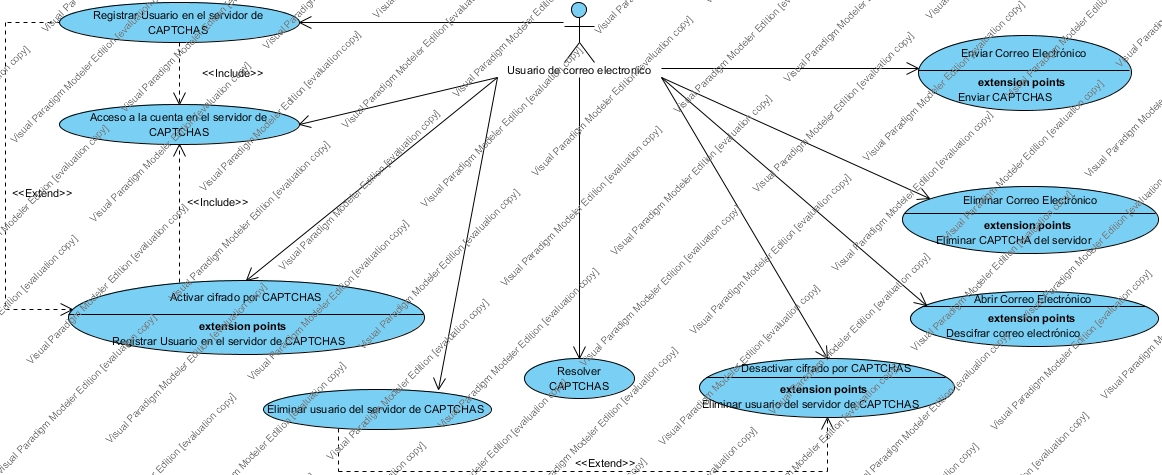
\includegraphics[width=1\linewidth, height=10cm]{./images/casodeuso1.jpg}
	\caption{Diagrama General de caso de uso}
	\label{fig:4-2-1}
\end{figure}
\subsection{Diagrama de casos de uso CU2 Registrar usuario en el servidor de CAPTCHAS}
\begin{figure}[H]
	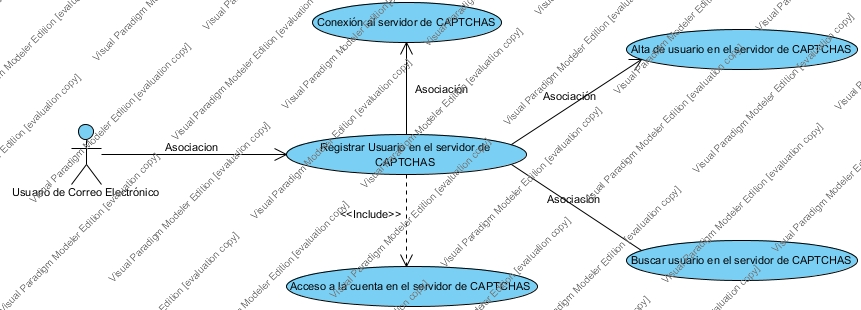
\includegraphics[width=1\linewidth, height=10cm]{./images/casodeuso2.jpg}
	\caption{Diagrama de casos de uso CU2 Registrar usuario en el servidor de CAPTCHAS}
	\label{fig:4-3-1}
\end{figure}

 \begin{longtable}[H]{| p{4,5cm} | p{0,5cm} |p{4cm}|p{5cm}|}%\footnotesize
   %\centering
   %{
     %\begin{tabular}
     \hline
     \textbf{Caso de Uso} &\multicolumn{3}{|l|}{CU2 Registrar Usuario en el servidor de CAPTCHAS}\\
     \hline
     \textbf{Actor} & \multicolumn{3}{|l|}{Actor1. Usuario de Correo Electrónico}\\
     \hline
     \textbf{Descripción} & \multicolumn{3}{|p{10cm}|}{Describe los pasos necesarios para registrar un nuevo usuario en el servidor de CAPTCHAS.}\\
     \hline
     \textbf{Pre-condiciones} & \multicolumn{3}{|l|}{Tener una cuenta de correo electrónico.}\\
     \hline
     \textbf{Post-condiciones} & \multicolumn{3}{|l|}{Activación del módulo de cifrado por CAPTCHAS.}\\
     \hline
     \textbf{Puntos de inclusión} & \multicolumn{3}{|l|}{Acceso a la cuenta en el servidor de CAPTCHAS.}\\
     \hline
     \textbf{Puntos de extensión} & \multicolumn{3}{|l|}{}\\
     \hline
     \textbf{Flujo principal} & & Actor/Sistema & Acción a realizar\\
     \hline
     & 1 & Actor & El usuario selecciona la opción registrarse en el servidor de CAPTCHAS\\
     \hline
     & 2 & Sistema & El cliente de correo contesta un formulario con la información necesaria para dar de alta en el servidor de CAPTCHAS.\\
     \hline
     & 3 & Actor & Completa el formulario y oprime el botón de registrar.\\
     \hline
     & 4 & Sistema & El sistema valida los datos proporcionados por el usuario.\\
     \hline
     & 5 & Sistema & Se conecta con el servidor y valida si el usuario ya está registrado. <FA01 - Usuario ya registrado> <FA02 - Falla en la conexión con el servidor>\\
     \hline
     & 6 & Sistema & Manda la información del usuario y lo da de alta.\\
     \hline
     & 7 & Sistema & Despliega el siguiente mensaje ``El usuario se ha dado de alta correctamente''\\
     \hline
     & & & \textbf{Fin del flujo principal}.\\
     \hline
     & \multicolumn{3}{|l|}{\textbf{FA01 - Usuario ya registrado}.}\\
     \hline
     \textbf{Flujo alternativo} & & Actor/Sistema & Acción a realizar\\
     \hline
     & 1 & Sistema & Despliega el siguiente mensaje  ``El usuario ya está registrado favor de proporcionar otra cuenta de correo electrónico''\\
     \hline
     & 2 & & El flujo continúa en el paso 3 del flujo principal.\\
     \hline
     &  & & \textbf{Fin del flujo alternativo}\\
     \hline
     
     \hline
     & \multicolumn{3}{|l|}{\textbf{FA02 - Falla en la conexión con el servidor}.}\\
     \hline
     \textbf{Flujo alternativo} & & Actor/Sistema & Acción a realizar\\
     \hline
     & 1 & Sistema & Despliega el siguiente mensaje ``La conexión con la red es nula o limitada, favor de realizar esta operación más tarde''\\
     \hline
     & 2 & & El flujo continúa en el paso 1 del flujo principal.\\
     \hline
     &  & & \textbf{Fin del flujo alternativo}\\
     %\end{tabular}
    %}
    \hline
    \caption{Descripción CU2.}
    \label{tabla:CU2}
\end{longtable}


\subsection{Diagrama de casos de uso CU3 Acceso a la cuenta en el servidor de CAPTCHAS}
\begin{figure}[H]
	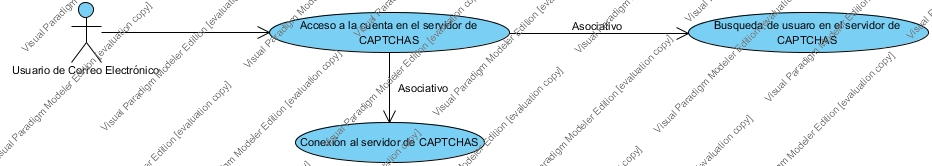
\includegraphics[width=1\linewidth, height=5cm]{./images/casodeuso3.jpg}
	\caption{Diagrama de casos de uso CU3 Acceso a la cuenta en el servidor de CAPTCHAS}
	\label{fig:4-4-1}
\end{figure}

\begin{longtable}[H]{| p{4,5cm} | p{0,5cm} |p{4cm}|p{5cm}|}
%\centering
   %{
     %\begin{tabular}{| p{4,5cm} | p{0,5cm} |p{4cm}|p{5cm}|}
     \hline
     \textbf{Caso de Uso} &\multicolumn{3}{|l|}{CU3 Acceso a la cuenta en el servidor de CAPTCHAS}\\
     \hline
     \textbf{Actor} & \multicolumn{3}{|l|}{Actor 1. Usuario de correo electrónico}\\
     \hline
     \textbf{Descripción} & \multicolumn{3}{|p{10cm}|}{Describe los pasos necesarios para dar acceso al los archivos guardados en el servidor de CAPTCHAS.}\\
     \hline
     \textbf{Pre-condiciones} & \multicolumn{3}{|p{10cm}|}{Tener una cuenta de correo electrónico.}\\
     \hline
     \textbf{Post-condiciones} & \multicolumn{3}{|l|}{Activación del modulo de cifrado por CAPTCHAS.}\\
     \hline
     \textbf{Puntos de inclusión} & \multicolumn{3}{|l|}{Desempaquetar correo electrónico}\\
     \hline
     \textbf{Puntos de extensión} & \multicolumn{3}{|l|}{Descifrar correo electrónico}\\
     \hline
     \textbf{Flujo principal} & & Actor/Sistema & Acción a realizar\\
     \hline
     & 1 & Actor & El usuario ingresa su correo electrónico, nombre de usuario y contraseña.\\
     \hline
     & 2 & Sistema & El cliente de correo abre una conexión con el servidor de CAPTCHAS.<FA01. Servidor no responde.>\\
     \hline
     & 3 & Sistema & El cliente de correo envía los datos ingresados por  el actor al servidor de CAPTCHAS.<FA02. Datos erróneos.>\\
     \hline
     & 4 & Sistema & Envía la respuesta satisfactoria al usuario.\\
     \hline
     & & & \textbf{Fin del flujo principal}.\\
     \hline
     & \multicolumn{3}{|l|}{\textbf{FA01 - Servidor no responde.}.}\\
     \hline
     \textbf{Flujo alternativo} & & Actor/Sistema & Acción a realizar\\
     \hline
     & 1 & Sistema & Despliega el siguiente mensaje "No se pudo establecer comunicación con el servidor de CAPTCHAS"\\
     \hline
     & & & \textbf{El flujo continua en el paso 1 del flujo principal.}\\
     \hline
     & & & \textbf{Fin del flujo alternativo}\\
     \hline
     & \multicolumn{3}{|l|}{\textbf{FA02 - Datos erróneos.}.}\\
     \hline
     \textbf{Flujo alternativo} & & Actor/Sistema & Acción a realizar\\
     \hline
     & 1 & Sistema & Despliega el siguiente mensaje " Los datos ingresados son inválidos"\\
     \hline
     & & & \textbf{El flujo continua en el paso 1 del flujo principal.}\\
     \hline
     & & & \textbf{Fin del flujo alternativo}\\
     \hline
     %\end{tabular}
    %}
    \caption{Descripción CU3.}
    \label{tabla:CU3}
\end{longtable}



\subsection{Diagrama de casos de uso CU4 Abrir Correo Electrónico.}
\begin{figure}[H]
	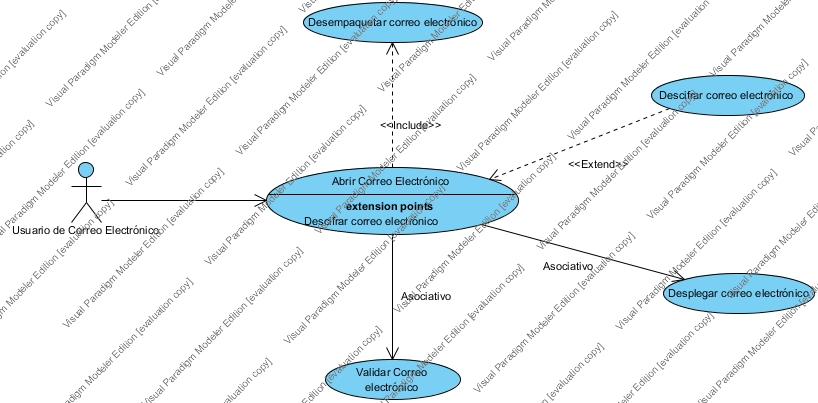
\includegraphics[width=1\linewidth, height=10cm]{./images/casodeuso4.jpg}
	\caption{Diagrama de casos de uso CU4 Abrir Correo Electrónico.}
	\label{fig:4-5-1}
\end{figure}
\pagebreak
\begin{longtable}[H]{| p{4,5cm} | p{0,5cm} |p{4cm}|p{5cm}|}
%\centering
   %{
     %\begin{tabular}{| p{4,5cm} | p{0,5cm} |p{4cm}|p{5cm}|}
     \hline
     \textbf{Caso de Uso} &\multicolumn{3}{|l|}{CU4 Abrir correo electrónico}\\
     \hline
     \textbf{Actor} & \multicolumn{3}{|l|}{Actor 1. Usuario de correo electrónico}\\
     \hline
     \textbf{Descripción} & \multicolumn{3}{|p{10cm}|}{Describe los pasos necesarios para abrir un mensaje de correo electrónico.}\\
     \hline
     \textbf{Pre-condiciones} & \multicolumn{3}{|p{10cm}|}{1. Iniciar sesión con su servidor de correo electrónico. 2. Descargar el correo electrónico que se desea abrir.}\\
     \hline
     \textbf{Post-condiciones} & \multicolumn{3}{|l|}{Despliegue del mensaje de correo electrónico descifrado.}\\
     \hline
     \textbf{Puntos de inclusión} & \multicolumn{3}{|l|}{Desempaquetar correo electrónico}\\
     \hline
     \textbf{Puntos de extensión} & \multicolumn{3}{|l|}{Descifrar correo electrónico}\\
     \hline
     \textbf{Flujo principal} & & Actor/Sistema & Acción a realizar\\
     \hline
     & 1 & Actor & El caso de uso comienza cuando el usuario selecciona el correo que desea abrir.\\
     \hline
     & 2 & Sistema & El sistema manda a llamar a la función de desempaquetar correo electrónico.\\
     \hline
     & 3 & Sistema & Valida si el mensaje viene timbrado. <FA01 - El mensaje no viene timbrado>\\
     \hline
     & 4 & Sistema & Invoca al caso de uso <CU Descifrar correo electrónico>\\
     \hline
     & 5 & Sistema & Recibe el mensaje de correo electrónico descifrado\\
     \hline
     & 6 & Sistema & Despliega el contenido completo del mensaje al usuario\\
     \hline
     & & & \textbf{Fin del flujo principal}.\\
     \hline
     & \multicolumn{3}{|l|}{\textbf{FA01 - El mensaje no viene timbrado}.}\\
     \hline
     \textbf{Flujo alternativo} & & Actor/Sistema & Acción a realizar\\
     \hline
     & 1 & Sistema & El flujo continúa en el paso 6 del flujo principal.\\
     \hline
     &  & & \textbf{Fin del flujo alternativo}\\
     \hline
     %\end{tabular}
    %}
    \caption{Descripción CU4.}
    \label{tabla:CU4}
\end{longtable}


\pagebreak

\subsection{Diagrama casos de uso CU5 Activar cifrado por CAPTCHAS.}
\begin{figure}[H]
	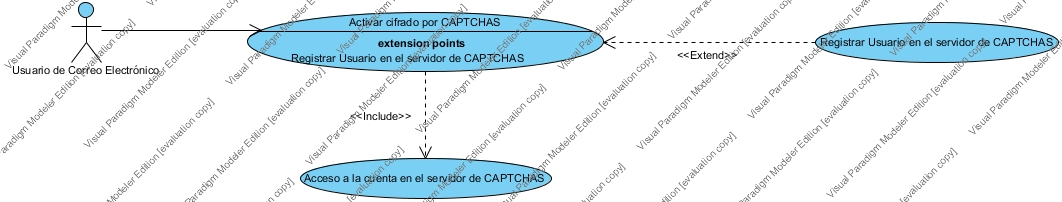
\includegraphics[width=1\linewidth, height=5cm]{./images/casodeuso5.jpg}
	\caption{Diagrama casos de uso CU5 Activar cifrado por CAPTCHAS.}
	\label{fig:4-6-1}
\end{figure}
\begin{longtable}[H]{| p{4,5cm} | p{0,5cm} |p{4cm}|p{5cm}|}
 %\centering
   %{
     %\begin{tabular}
     \hline
     \textbf{Caso de Uso} &\multicolumn{3}{|l|}{CU5 Activar cifrado por CAPTCHAS}\\
     \hline
     \textbf{Actor} & \multicolumn{3}{|l|}{Actor 1. Usuario de correo electrónico}\\
     \hline
     \textbf{Descripción} & \multicolumn{3}{|p{10cm}|}{Describe los pasos necesarios para activar el módulo de cifrado CAPTCHAS en el cliente de correo electrónico.}\\
     \hline
     \textbf{Pre-condiciones} & \multicolumn{3}{|l|}{1. Instalar el módulo de cifrado por CAPTCHAS}\\
     \hline
     \textbf{Post-condiciones} & \multicolumn{3}{|l|}{Activación del cifrado y descifrado por CAPTCHAS.}\\
     \hline
     \textbf{Puntos de inclusión} & \multicolumn{3}{|l|}{}\\
     \hline
     \textbf{Puntos de extensión} & \multicolumn{3}{|l|}{Registrar usuario del servidor de CAPTCHAS}\\
     \hline
     \textbf{Flujo principal} & & Actor/Sistema & Acción a realizar\\
     \hline
     & 1 & Actor & El caso de uso inicia cuando el actor seleccionar la opción ``Activar cifrado por CAPTCHAS''\\
     \hline
     & 2 & Sistema & El sistema verifica si la dirección de correo del usuario está registrada en el servidor de CAPTCHAS<FA01 -Usuario no registrado en el servidor>\\
     \hline
     & 3 & Sistema & Despliega una ventana con el mensaje ``Activación del módulo de cifrado por CAPTCHAS''\\
     \hline
     & & & \textbf{Fin del flujo principal}.\\
     \hline
     & \multicolumn{3}{|l|}{\textbf{FA01 -Usuario no registrado en el servidor}.}\\
     \hline
     \textbf{Flujo alternativo} & & Actor/Sistema & Acción a realizar\\
     \hline
     & 1 & Sistema & El sistema despliega una ventana con las opciones de ``Registrarse'' y ``Cancelar''. <FA02 Cancelar activación>\\
     \hline
     & 2 & Actor & Oprime el botón de ``Registrarse''\\
     \hline
     & 3 & Sistema & El sistema invoca al caso de uso <CU Registrar usuario en el servidor de CAPTCHAS>\\
     \hline
     & 4 & Sistema & El sistema obtiene una respuesta satisfactoria del registro\\
     \hline
     & 5 &  & El flujo continúa en el paso 2 del flujo principal.\\
     \hline
     &  & & \textbf{Fin del flujo alternativo}\\
     \hline
     & \multicolumn{3}{|l|}{\textbf{FA02 - Cancelar activación}.}\\
     \hline
     \textbf{Flujo alternativo} & & Actor/Sistema & Acción a realizar\\
     \hline
     & 1 & Actor & El Actor selecciona ``Cancelar''\\
     \hline
     & 2 & Sistema & Cierra la ventana de selección\\
     \hline
     & 3 &  & El flujo continúa en el paso 1 del flujo principal.\\
     \hline
     &  & & \textbf{Fin del flujo alternativo}\\
     %\end{tabular}
    %}
    \hline
    \caption{Descripción CU5.}
    \label{tabla:CU5}
\end{longtable}

\subsection{Diagrama de casos de uso CU6 Descifrar correo electrónico.}
\begin{figure}[H]
	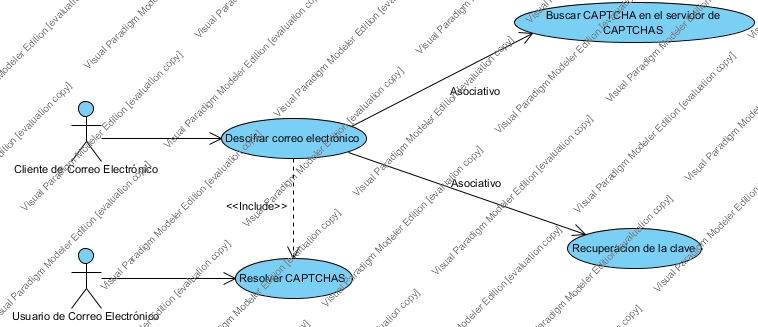
\includegraphics[width=1\linewidth, height=7cm]{./images/casodeuso6.jpg}
	\caption{Diagrama de casos de uso CU6 Descifrar correo electrónico.}
	\label{fig:4-7-1}
\end{figure}
\pagebreak
\begin{longtable}[H]{| p{4,5cm} | p{0,5cm} |p{4cm}|p{5cm}|}
 %\centering
   %{
     %\begin{tabular}
     \hline
     \textbf{Caso de Uso} &\multicolumn{3}{|l|}{CU6 Descifrar correo electrónico.}\\
     \hline
     \textbf{Actor} & \multicolumn{3}{|l|}{Actor 1. Usuario de correo electrónico}\\
     \hline
     \textbf{Descripción} & \multicolumn{3}{|p{10cm}|}{Describe los pasos necesarios para desactivar el módulo de cifrado CAPTCHAS en el cliente de correo electrónico}\\
     \hline
     \textbf{Pre-condiciones} & \multicolumn{3}{|p{10cm}|}{1. Activar cifrado por CAPTCHAS. 2. Registrar usuario en el servidor de CAPTCHAS}\\
     \hline
     \textbf{Post-condiciones} & \multicolumn{3}{|l|}{Desactivación del cifrado y descifrado por CAPTCHAS.}\\
     \hline
     \textbf{Puntos de inclusión} & \multicolumn{3}{|l|}{}\\
     \hline
     \textbf{Puntos de extensión} & \multicolumn{3}{|l|}{Eliminar usuario del servidor de CAPTCHAS}\\
     \hline
     \textbf{Flujo principal} & & Actor/Sistema & Acción a realizar\\
     \hline
     & 1 & Actor & El caso de uso inicia cuando el actor seleccionar la opción "Desactivar cifrado por CAPTCHAS"\\
     \hline
     & 2 & Sistema & El sistema despliega la venta con las opciones de ``Desactivar cifrado'' y ``Eliminar usuario'' <FA01 - Eliminar usuario>\\
     \hline
     & 3 & Actor & Selecciona la Desactivación del cifrado por CAPTCHAS\\
     \hline
     & 4 & Sistema & El sistema desactiva el módulo de cifrado por CAPTCHA\\
     \hline
     & & & \textbf{Fin del flujo principal}.\\
     \hline
    & \multicolumn{3}{|l|}{\textbf{FA01 - Eliminar usuario}.}\\
    \hline
    \textbf{Flujo alternativo} & & Actor/Sistema & Acción a realizar\\
    \hline
    & 1 & Actor & El Actor selecciona ``Eliminar usuario''\\
    \hline
    & 2 & Sistema & El sistema despliega una ventana con las opciones de ``Aceptar'' y ``Cancelar'' para confirmar la eliminación del usuario. <FA02 - Cancelar acción eliminar usuario>\\
    \hline
     & 3 & Actor & Oprime el botón de ``Aceptar''\\
     \hline
     & 4 & Sistema & Establece la conexión con el servidor de CAPTCHAS <FA03 - Fallo en la conexión con el servidor>\\
     \hline
     & 5 & Sistema & Busca y elimina al usuario de la base de datos desplegando la confirmación del servidor.\\
     \hline
     & 6 & Actor & Oprime el botón de ``Aceptar''\\
     \hline
     & 7 & Sistema & Desactiva el módulo de cifrado por CAPTCHA\\
     \hline
     &  & & \textbf{Fin del flujo alternativo}\\
     \hline
     & \multicolumn{3}{|l|}{\textbf{FA02 - Cancelar acción eliminar usuario}.}\\
    \hline
    \textbf{Flujo alternativo} & & Actor/Sistema & Acción a realizar\\
    \hline
    & 1 & Actor & El Actor selecciona ``Cancelar''\\
    \hline
    & 2 & Sistema & Cierra la ventana de confirmación\\
    \hline
    &  & & \textbf{Fin del flujo alternativo}\\
     \hline
    & \multicolumn{3}{|l|}{\textbf{FA03 - Fallo en la conexión con el servidor}.}\\
    \hline
    \textbf{Flujo alternativo} & & Actor/Sistema & Acción a realizar\\
    \hline
    & 1 & Sistema & Despliega una ventana de alerta con el mensaje ``No se ha podido establecer la conexión con el servidor, es probable que no se tenga conexión a internet. Favor de intentarlo más tarde''\\
    \hline
    & 2 & Actor & Cierra la ventana de alerta\\
    \hline
    & 3 &  & El flujo continúa en el paso 1 del flujo principal\\
    \hline
    &  & & \textbf{Fin del flujo alternativo}\\
    % \end{tabular}
    %}
    \hline
    \caption{Descripción CU6.}
    \label{tabla:CU6}
\end{longtable}


\pagebreak

\subsection{Diagrama de casos de uso CU7 Enviar CAPTCHAS}
\begin{figure}[H]
	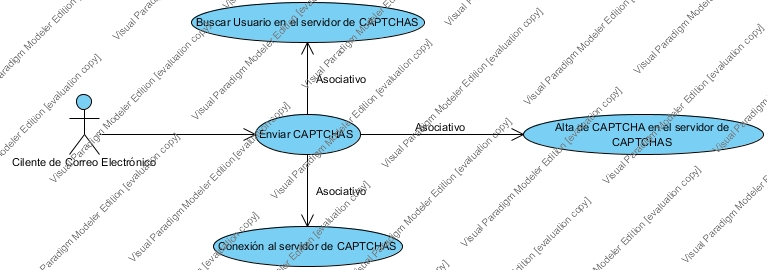
\includegraphics[width=1\linewidth, height=8cm]{./images/casodeuso9.jpg}
	\caption{Diagrama de casos de uso CU7 Enviar CAPTCHAS}
	\label{fig:4-10-1}
\end{figure}

\begin{longtable}[H]{| p{4,5cm} | p{0,5cm} |p{4cm}|p{5cm}|}
 %\centering
   %{
     %\begin{tabular}{| p{4,5cm} | p{0,5cm} |p{4cm}|p{5cm}|}
     \hline
     \textbf{Caso de Uso} &\multicolumn{3}{|l|}{CU7 Enviar CAPTCHAS}\\
     \hline
     \textbf{Actor} & \multicolumn{3}{|l|}{Actor 1. Cliente de correo electrónico.}\\
     \hline
     \textbf{Descripción} & \multicolumn{3}{|p{10cm}|}{Describe los pasos necesarios para enviar el CAPTCHA el servidor de CAPTCHAS}\\
     \hline
     \textbf{Pre-condiciones} & \multicolumn{3}{|l|}{1. Solicitar el envió de un nuevo mensaje de correo electrónico.}\\
     \hline
     \textbf{Post-condiciones} & \multicolumn{3}{|l|}{Envío del CAPTCHA al servidor de CAPTCHAS}\\
     \hline
     \textbf{Puntos de inclusión} & \multicolumn{3}{|l|}{}\\
     \hline
     \textbf{Puntos de extensión} & \multicolumn{3}{|l|}{}\\
     \hline
     \textbf{Flujo principal} & & Actor/Sistema & Acción a realizar\\
     \hline
     & 1 & Actor & Solicita el envío de CAPTCHA al servidor\\
     \hline
     & 2 & Sistema & Abre la conexión y busca al usuario en el servidor de CAPTCHAS\\
     \hline
     & 3 & Sistema & Da de alta el CAPTCHA en el servidor asociándolo con el usuario.\\
     \hline
     & 4 & Sistema & Regresa la confirmación de que se dio de alta el CAPTCHA\\
     \hline
     & & & \textbf{Fin del flujo principal}.\\
     \hline
     %\end{tabular}
    %}
    \caption{Descripción CU7.}
    \label{tabla:CU7}
\end{longtable}


\pagebreak
\subsection{Diagrama de casos de uso CU8 Enviar correo electrónico.}
\begin{figure}[H]
	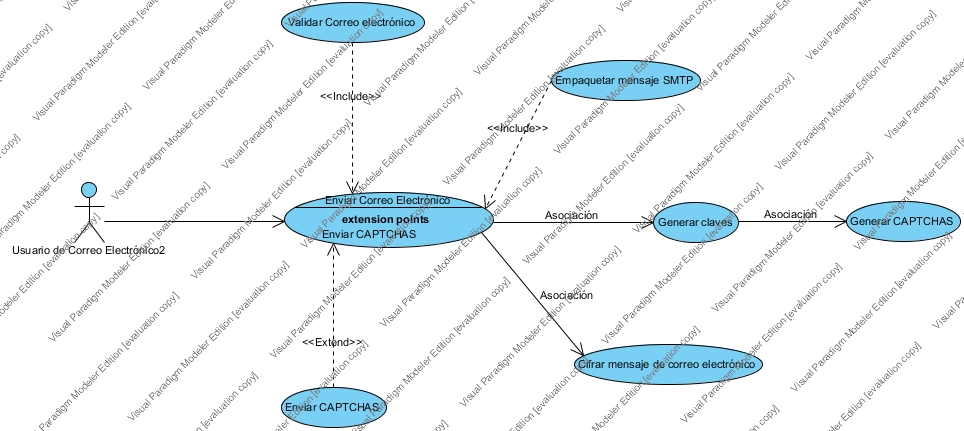
\includegraphics[width=1\linewidth, height=8cm]{./images/casodeuso10.jpg}
	\caption{Diagrama de casos de uso CU8 Enviar correo electrónico.}
	\label{fig:4-11-1}
\end{figure}
\begin{longtable}[H]{| p{4,5cm} | p{0,5cm} |p{4cm}|p{5cm}|}
 %\centering
   %{
     %\begin{tabular}{| p{4,5cm} | p{0,5cm} |p{4cm}|p{5cm}|}
     \hline
     \textbf{Caso de Uso} &\multicolumn{3}{|l|}{CU8 Enviar correo electrónico.}\\
     \hline
     \textbf{Actor} & \multicolumn{3}{|l|}{Actor 1. Usuario de correo electrónico.}\\
     \hline
     \textbf{Descripción} & \multicolumn{3}{|p{10cm}|}{Describe los pasos necesarios para enviar un mensaje de correo electrónico cifrado a otro usuario de correo electrónico.}\\
     \hline
     \textbf{Pre-condiciones} & \multicolumn{3}{|p{10cm}|}{1. El usuario tiene que redactar un mensaje de correo electrónico que contenga la dirección del destinatario.}\\
     \hline
     \textbf{Post-condiciones} & \multicolumn{3}{|p{10cm}|}{Envió de un mensaje cifrado al servidor de correo electrónico y el registro del CAPTCHA en el servidor de CAPTCHAS.}\\
     \hline
     \textbf{Puntos de inclusión} & \multicolumn{3}{|p{10cm}|}{1. Validar correo electrónico. 2. Empaquetar mensaje de correo electrónico SMTP.}\\
     \hline
     \textbf{Puntos de extensión} & \multicolumn{3}{|l|}{Enviar CAPTCHA}\\
     \hline
     \textbf{Flujo principal} & & Actor/Sistema & Acción a realizar\\
     \hline
     & 1 & Actor & Oprime el botón ``Enviar''\\
     \hline
     & 2 & Sistema & Valida que el mensaje de correo electrónico contenga los datos mínimos.<FA01 - Campos no completados>\\
     \hline
     & 3 & Sistema & Genera una llave de cifrado\\
     \hline
     & 4 & Sistema & Con una palabra aleatoria se genera el CAPTCHA y cifra el mensaje de correo electrónico.\\
     \hline
     & 5 & Sistema & Toma el mensaje cifrado y es empaquetado para enviarse al servidor de correo electrónico\\
     \hline
     & 6 & Sistema & Toma el CAPTCHA  y se envía al caso de uso <CU Enviar CAPTCHA>\\
     \hline
     & 7 & Sistema & Despliega el mensaje de ``envío satisfactorio''\\
     \hline
     & & & \textbf{Fin del flujo principal}.\\
     \hline
     & \multicolumn{3}{|l|}{\textbf{FA01 - Campos no completados}.}\\
     \hline
     \textbf{Flujo alternativo} & & Actor/Sistema & Acción a realizar\\
     \hline
     & 1 & Sistema & Notifica al usuario cuales campos han sido mal proporcionados, para poder enviar el mensaje correctamente\\
     \hline
     & 2 & Actor & Modifica los campos solicitados\\
     \hline
     & 3 &  & El flujo continúa en el paso 1 del flujo principal\\
     \hline
     &  & & \textbf{Fin del flujo alternativo}\\
     \hline
     %\end{tabular}
    %}
    \caption{Descripción CU8.}
    \label{tabla:CU8}
\end{longtable}



\pagebreak
\section{Diagramas a bloques}
A continuación se presentan los diagramas a bloques, en donde se muestra cuál es la secuencia de procesos a realizar. Esto servirá para comprender cómo se comunican los diferentes módulos de manera interna, y cómo hacen los procesos.


\begin{figure}[H]
	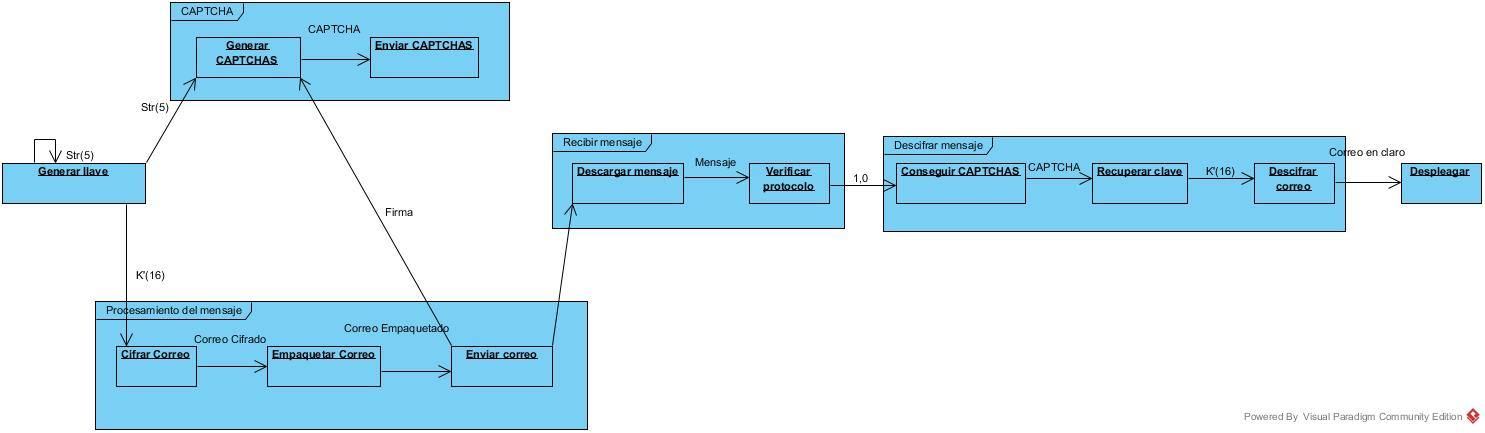
\includegraphics[width=1\linewidth, height=5cm]{./images/bloques0.jpg}
	\caption{Diagrama a bloque 0 general del sistema}
	\label{fig:5-1-1}
\end{figure}
\pagebreak
\begin{table}[H]
 \centering
   {
     \begin{tabular}{| p{2,2cm} | p{1,7cm} | p{2,5cm} | p{3cm} | p{2cm} | p{2,1cm} | p{2cm} |}
     \hline
     & \textbf{Generar clave} & \textbf{Generar CAPTCHA} & \textbf{Procesamiento del mensaje} & \textbf{Recibir mensaje} & \textbf{Descifrar mensaje} & \textbf{Desplegar}\\
     \hline
     \textbf{Entradas} & *Señal de activación & *Cadena de 5 caracteres: Str(5) & *Clave de 16 bytes: K’(16). *Mensaje de correo. & *Correo Cifrado & Verificación (1,0) & *Correo en claro\\
     \hline
     \textbf{Salidas} & *Cadena de 5 caracteres: Str(5) *Clave de 16 bytes: K’(16) & *Señal de envió & *Correo Cifrado & *Verificación (1,0) & *Correo en claro&\\
     \hline
     \textbf{Descripción} & Se activa el proceso generar clave, este crea una palabra de 5 caracteres (Str(5)), procesa la palabra Str(5) por medio de una función hash obteniendo una palabra de 256 caracteres (K(256)) y recorta esta clave a una palabra de 16 caracteres (K’(16)). & Toma la entrada Str(5) y la convierte en una imagen CAPTCHA, Posteriormente inicia una conexión con el servidor de CAPTCHAS para mandarlo a este. & Cifra el mensaje de correo con la clave K’(16), posteriormente lo firma y genera un timbre para saber que fue creado con este esquema y lo empaqueta para su envió. & El cliente hace una petición al servidor y descarga el mensaje de correo electrónico, lo des empaqueta verifica la firma y el timbrado para saber de quién viene y si está cifrado bajo este esquema. & Se hace una petición al servidor de CAPTCHAS, se descargan los CAPTCHAS asociados al correo, ya con el CAPTCHA este se resuelve y se recupera la cadena Str(5), esta se pasa por una función hash y se recupera K(256), esta se corta a K’(16), con esto se descifra el mensaje. & Se muestra el correo descifrado en la interfase del cliente de correo electrónico.\\
	\hline
    \end{tabular}
    }
    \caption{Diagrama a bloques 0 general}
    \label{tabla:b0}
\end{table}


\newpage
\newpage
\subsection{Diagrama a bloques 1 Generar clave}
\begin{figure}[H]
	
\includegraphics[width=1\linewidth, height=2cm]{./images/bloques1.jpg}
	\caption{Diagrama a bloques 1 Generar clave}
	\label{fig:5-2-1}
\end{figure}
\begin{table}[H]
 \centering
   {
     \begin{tabular}{| p{4cm} | p{4cm} | p{4cm} | p{4cm} |}
     \hline
     & \textbf{Generar Str(5)} & \textbf{Aplicar Función Hash} & \textbf{Recortar Hash K’}\\
     \hline
     \textbf{Entradas} & *Llamada a Función & *Cadena de 5 caracteres: Str(5) & *Digesto K(128)\\
     \hline
     \textbf{Salidas} & *Cadena de 5 caracteres: Str(5) & *Digesto K(128) & *K’(16)\\
     \hline
     \textbf{Descripción} & Toma una función random módulo 67, para formar una palabra con 5 caracteres aleatorios tomados del siguiente conjunto.Anillo67{-.,+*[a-z][A-Z]} & Se pasa la cadena Str(5) por una función hash SHA-1 para obtener un digesto único de esta palabra. & Se copian a otro string lo primeros 16 caracteres del digesto K(128) para formar la clave K’(16)\\
	\hline
    \end{tabular}
    }
    \caption{Diagrama a bloques 1 general clave}
    \label{tabla:b1}
\end{table}
\subsection{Diagrama a bloques 2 Cifrado}
\begin{table}[H]
 \centering
   {
     \begin{tabular}{| p{3cm} | p{3cm} |}
     \hline
     & \textbf{Cifrar}\\
     \hline
     \textbf{Entradas} & *Clave K’(16) *Mensaje de correo\\
     \hline
     \textbf{Salidas} & *Correo cifrado\\
     \hline
     \textbf{Descripción} & Se cifra el mensaje con un algoritmo de llave simétrica (AES o DES) usando una llave de 16bytes o 128bits.\\
	\hline
    \end{tabular}
    }
    \caption{Diagrama a bloques 2 Cifrar Correo}
    \label{tabla:b2}
\end{table}
\subsection{Diagrama a bloques 3 Empaquetar Correo}
\begin{figure}[H]
	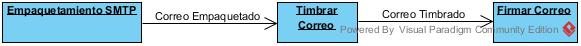
\includegraphics[width=1\linewidth, height=1cm]{./images/bloques3.jpg}
	\caption{Diagrama a bloques 3 Empaquetar Correo}
	\label{fig:5-3-1}
\end{figure}

\begin{table}[H]
 \centering
   {
     \begin{tabular}{| p{4cm} | p{4cm} | p{4cm} |}
     \hline
     & \textbf{Empaquetamiento SMTP} & \textbf{Timbrar Correo}\\
     \hline
     \textbf{Entradas} & *Mensaje Cifrado & *Correo Empaqueta\\
     \hline
     \textbf{Salidas} & *Correo Empaquetado & *Correo Timbrado\\
     \hline
     \textbf{Descripción} & Se toma el correo y se integra en el formato del correo marcado en el RFC822 & Se timbra el mensaje colocando una marca después del final del mensaje. Para señalar que el correo enviado está cifrado bajo este protocolo.\\
	\hline
    \end{tabular}
    }
    \caption{Diagrama a bloques 3 Empaquetar Correo}
    \label{tabla:b3}
\end{table}
\subsection{Diagrama a bloques 4 Enviar correo}
\begin{figure}[H]
	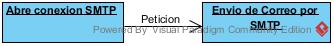
\includegraphics[width=1\linewidth, height=2cm]{./images/bloques4.jpg}
	\caption{Diagrama a bloques 4 Enviar correo}
	\label{fig:5-4-1}
\end{figure}

\begin{table}[H]
 \centering
   {
     \begin{tabular}{| p{4cm} | p{4cm} | p{4cm} |}
     \hline
     & \textbf{Abrir conexión SMTP} & \textbf{Envió de Correo por SMTP}\\
     \hline
     \textbf{Entradas} & *Petición & *Correo empaquetado\\
     \hline
     \textbf{Salidas} & *Canal de comunicación & *Confirmación de envió\\
     \hline
     \textbf{Descripción} & Se genera una petición para conexión SMTP  & Se manda el correo electrónico al servidor por medio del protocolo SMTP\\
	\hline
    \end{tabular}
    }
    \caption{Diagrama a bloques 4 Enviar correo}
    \label{tabla:b4}
\end{table}
\clearpage
\subsection{Diagrama a bloques 5 Generar CAPTCHA}
\begin{figure}[H]
	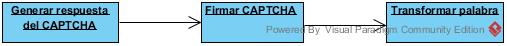
\includegraphics[width=1\linewidth, height=2cm]{./images/bloques5.jpg}
	\caption{Diagrama a bloques 5 Generar CAPTCHA}
	\label{fig:5-5-1}
\end{figure}
\begin{table}[H]
 \centering
   {
     \begin{tabular}{| p{4cm} | p{4cm} | p{4cm} | p{4cm} |}
     \hline
     & \textbf{Generar respuesta del CAPTCHA} & \textbf{Firmar CAPTCHA} & \textbf{Transformar palabra}\\
     \hline
     \textbf{Entradas} & *Cadena de caracteres: Str(5) & *Firma & *Señal de confirmación\\
     \hline
     \textbf{Salidas} & *Señal de confirmación & *Archivo Firmado & *Imagen CAPTCHA\\
     \hline
     \textbf{Descripción} & Genera un archivo con la respuesta del CAPTCHA  & Se firma el CAPTCHA por medio de un Hashing del mensaje. & Convierte el Str(5) en una imagen distorsionada que llamaremos CAPTCHA\\
	\hline
    \end{tabular}
    }
    \caption{Diagrama a bloques 5 Generar CAPTCHA}
    \label{tabla:b5}
\end{table}

\subsection{Diagrama a bloques 6 Enviar CAPTCHAS}
\begin{figure}[H]
	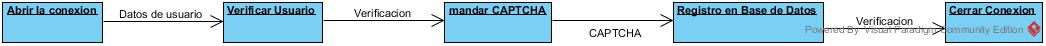
\includegraphics[width=1\linewidth, height=1cm]{./images/bloques6.jpg}
	\caption{Diagrama a bloques 6 Enviar CAPTCHAS (Usuario existente)}
	\label{fig:5-6-1}
\end{figure}

\begin{table}[H]
 \centering
   {
     \begin{tabular}{| p{2,5cm} | p{2,5cm} | p{2,5cm} | p{2,5cm} | p{2,5cm} | p{2,5cm} |}
     \hline
     & \textbf{Abrir conexión} & \textbf{Verificar Usuario} & \textbf{Mandar CAPTCHA} & \textbf{Registrar en base de datos} & \textbf{Cerrar Conexión}\\
     \hline
     \textbf{Entradas} & *CAPTCHAS & *Datos de Usuario & *Verificación de usuario & *Datos de usuario *CAPTCHA & Verificación\\
     \hline
     \textbf{Salidas} & *Datos de usuario & *Verificación de usuario & *CAPTCHA & Verificación &\\
     \hline
     \textbf{Descripción} & Se genera una petición para poder entablar una conexión con el servidor de CAPTCHAS & Se verifica la existencia del usuario en el servidor, si existe se le da acceso & Ya verificado el usuario se manda el CAPTCHA al servidor & Se registran los datos del CAPTCHA en la base de datos y se envía una verificación & Se cierra la conexión y se guardan los datos\\
	\hline
    \end{tabular}
    }
    \caption{Diagrama a bloques 6 Enviar CAPTCHAS (Usuario existente)}
    \label{tabla:b6}
\end{table}

\subsection{Diagrama a bloques 7 Enviar CAPTCHAS}
\begin{figure}[H]
	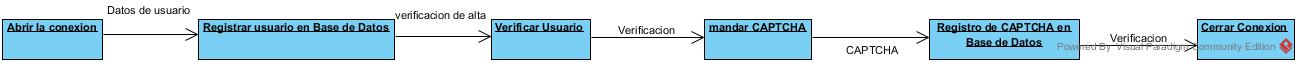
\includegraphics[width=1\linewidth, height=1cm]{./images/bloques7.jpg}
	\caption{Diagrama a bloques 7 Enviar CAPTCHAS (Usuario inexistente)}
	\label{fig:5-7-1}
\end{figure}
\begin{table}[H]
 \centering
   {
     \begin{tabular}{| p{2cm} | p{2cm} | p{2,5cm} | p{2cm} | p{2,5cm} | p{2,5cm} | p{2cm} |}
     \hline
     & \textbf{Abrir conexión} & \textbf{Registrar usuario en Base de Datos} & \textbf{Verificar Usuario} & \textbf{Mandar CAPTCHA} & \textbf{Registrar en base de datos} & \textbf{Cerrar Conexión}\\
     \hline
     \textbf{Entradas} & *CAPTCHAS & *Datos de Usuario & *Verificación de registro & *Verificación de usuario & *Datos de usuario *CAPTCHA & Verificación\\
     \hline
     \textbf{Salidas} & *Datos de usuario & *Verificación de registro & *Verificación de usuario & *CAPTCHA & Verificación &\\
     \hline
     \textbf{Descripción} & Se genera una petición para poder entablar una conexión con el servidor de CAPTCHAS & Se da de alta al usuario en la base de datos & se le da acceso  al usuario & Ya verificado el usuario se manda el CAPTCHA al servidor & Se registran los datos del CAPTCHA en la base de datos y se envía una verificación & Se cierra la conexión y se guardan los datos\\
	\hline
    \end{tabular}
    }
    \caption{Diagrama a bloques 7 Enviar CAPTCHAS (Usuario inexistente)}
    \label{tabla:b7}
\end{table}
\pagebreak
\subsection{Diagrama a bloques 8 Descargar mensaje}
\begin{figure}[H]
	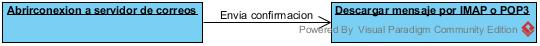
\includegraphics[width=1\linewidth, height=1cm]{./images/bloques8.jpg}
	\caption{Diagrama a bloques 8 Descargar mensaje}
	\label{fig:5-8-1}
\end{figure}
\begin{table}[H]
 \centering
   {
     \begin{tabular}{| p{3cm} | p{4cm} | p{4cm} |}
     \hline
     & \textbf{Abrir conexión al servidor de correo} & \textbf{Descargar mensaje por IMAP o POP3}\\
     \hline
     \textbf{Entradas} & *Señal de activación & *Confirmación\\
     \hline
     \textbf{Salidas} & *Confirmación & *Correo electrónico\\
     \hline
     \textbf{Descripción} & El receptor se conecta al servidor de correo electrónico e inicia la sesión & Descarga del servidor de correo electrónico todos los mensajes que aún no se hayan descargado.\\
	\hline
    \end{tabular}
    }
    \caption{Diagrama a bloques 8 Descargar mensaje}
    \label{tabla:b8}
\end{table}
\subsection{Diagrama a bloques 9 Verificar protocolo}
\begin{figure}[H]
	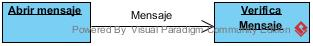
\includegraphics[width=1\linewidth, height=1cm]{./images/bloques9.jpg}
	\caption{Diagrama a bloques 9 Verificar protocolo (con protocolo válido)}
	\label{fig:5-9-1}
\end{figure}
\begin{table}[H]
 \centering
   {
     \begin{tabular}{| p{3cm} | p{4cm} | p{4cm} |}
     \hline
     & \textbf{Abrir mensaje} & \textbf{Verificar mensaje}\\
     \hline
     \textbf{Entradas} & *Correo electrónico & *mensaje\\
     \hline
     \textbf{Salidas} & *Mensaje & *verificación\\
     \hline
     \textbf{Descripción} & Se toma el mensaje descargado del servidor y se des empaqueta para dejar solo el texto del mensaje & Se verifica que el mensaje tenga la bandera correspondiente a que está cifrado con este esquema\\
	\hline
    \end{tabular}
    }
    \caption{Diagrama a bloques 9 Verificar protocolo (con protocolo válido)}
    \label{tabla:b9}
\end{table}
\pagebreak
\subsection{Diagrama a bloques 10 Verificar protocolo}
\begin{figure}[H]
	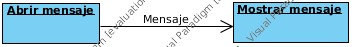
\includegraphics[width=1\linewidth, height=1cm]{./images/bloques10.jpg}
	\caption{Diagrama a bloques 10 Verificar protocolo (con protocolo inválido)}
	\label{fig:5-9-1}
\end{figure}
\begin{table}[H]
 \centering
   {
     \begin{tabular}{| p{3cm} | p{4cm} | p{4cm} |}
     \hline
     & \textbf{Abrir mensaje} & \textbf{Verificar mensaje}\\
     \hline
     \textbf{Entradas} & *Correo electrónico & *mensaje\\
     \hline
     \textbf{Salidas} & *Mensaje & *verificación\\
     \hline
     \textbf{Descripción} & Se toma el mensaje descargado del servidor y se des empaqueta para dejar solo el texto del mensaje & Si la verificación es negativa se manda directamente al bloque de Despliegue\\
	\hline
    \end{tabular}
    }
    \caption{Diagrama a bloques 10 Verificar protocolo (con protocolo inválido)	}
    \label{tabla:b10}
\end{table}

\subsection{Diagrama a bloques 11 Conseguir CAPTCHAS}
\begin{figure}[H]
	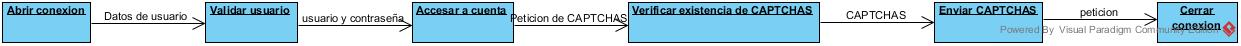
\includegraphics[width=1\linewidth, height=1cm]{./images/bloques11.jpg}
	\caption{Diagrama a bloques 11 Conseguir CAPTCHAS (Usuario existente)}
	\label{fig:5-11-1}
\end{figure}
\begin{table}[H]
 \centering
   {
     \begin{tabular}{| p{2,5cm} | p{3cm} | p{2cm} | p{2cm} | p{3cm} | p{3cm} |}
     \hline
     & \textbf{Abrir Conexión} & \textbf{Validar Usuario} & \textbf{Accesar a cuenta} & \textbf{Verificar existencia de CAPTCHA} & \textbf{Enviar CAPTCHA}\\
     \hline
     \textbf{Entradas} & *Confirmación & *Datos usuario & *Contraseña & *Petición de CAPTCHAS & *Confirmación\\
     \hline
     \textbf{Salidas} & *verificación & *Contraseña & *confirmación & *confirmación & *CAPTCHA\\
     \hline
     \textbf{Descripción} & Se abre una conexión con el servidor de CAPTCHAS & Se verifica que el usuario este dado de alta en el servidor mandándole una petición a la base de datos, si el usuario existe se accesa & Si esta dado de alta en el servidor se manda la contraseña para que pueda tener acceso a los CAPTCHAS de su cuenta & Se verifica que los CAPTCHAS que están ligados al mensaje que realizo la petición existan & Si existen estos CAPTCHAS son enviados de regreso al mensaje\\
	\hline
    \end{tabular}
    }
    \caption{Diagrama a bloques 11 Conseguir CAPTCHAS (Usuario existente)}
    \label{tabla:b11}
\end{table}

\subsection{Diagrama a bloques 12 Recuperar clave}
\begin{figure}[H]
	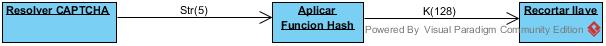
\includegraphics[width=1\linewidth, height=1cm]{./images/bloques12.jpg}
	\caption{Diagrama a bloques 12 Recuperar clave}
	\label{fig:5-12-1}
\end{figure}
\begin{table}[H]
 \centering
   {
     \begin{tabular}{| p{2,5cm} | p{3cm} | p{3cm} | p{3cm} |}
     \hline
     & \textbf{Resolver CAPTCHA} & \textbf{Aplicar Función Hash} & \textbf{Recortar llave}\\
     \hline
     \textbf{Entradas} & *CAPTCHA & *Cadena de 5 caracteres: Str(5) & *Digesto K(128)\\
     \hline
     \textbf{Salidas} & *Str(5) & *Digesto K(128) & *K’(16)\\
     \hline
     \textbf{Descripción} & Se despliega el CAPTCHA para que el usuario pueda resolverlo & Se pasa la cadena Str(5) por una función hash SHA-1 para obtener un digesto único de esta palabra & Se copian a otro string lo primeros 16 caracteres del digesto K(128) para formar la clave K’(16)\\
	\hline
    \end{tabular}
    }
    \caption{Diagrama a bloques 12 Recuperar clave}
    \label{tabla:b12}
\end{table}

\subsection{Diagrama a bloques 13 Descifrar correo}
\begin{table}[H]
 \centering
   {
     \begin{tabular}{| p{2,5cm} | p{3cm} |}
     \hline
     & \textbf{Descifrar}\\
     \hline
     \textbf{Entradas} & *Clave K’(16) *Mensaje de correo\\
     \hline
     \textbf{Salidas} & *Correo descifrado\\
     \hline
     \textbf{Descripción} & Se descifra el mensaje con un algoritmo de llave simétrica (AES o DES) usando una llave de 16bytes o 128bits.\\
	\hline
    \end{tabular}
    }
    \caption{Diagrama a bloques 13 Descifrar correo}
    \label{tabla:b13}
\end{table}
%\chapter{Desarrollo de prototipos}

\section{Prototipo 1}
\textbf{Objetivo del prototipo}:
Conocer el uso, funcionamiento e implementación de herramientas de cifrado, hashing y generación de CAPTCHAS, con el fin de conocer la integración de estos módulos en diferentes lenguajes de programación.\\
Se implementó un módulo de cifrado de mensajes de texto en lenguaje C++. Tratando de simular el proceso de cifrado del esquema que se esta usando.\\
La primera parte del proceso es abrir el mensaje para lo cual se estan usando los métodos estándar definidos en las bibliotecas nativas de C++, posteriormente se generará una palabra aleatoria de 5 caracteres usando una función Rand()\%100 y transformando el valor de salida a un char.\\
Al resultado se pasa por una función de hashing, esta función no es nativa de ninguna biblioteca estándar de C++ ni de C, por lo que se tuvo que conseguir una en internet y probar que efectivamente funcionara como se necesita.\\
Posteriormente este hash se usará como clave para cifrar el mensaje que ya se ha abierto, para esto se necesita una función AES o DES, ninguna de estas es estándar de alguna biblioteca de C o C++, así que se tendra que buscar y verificar su funcionamiento.\\


\textbf{Conclusión}:
Podemos ver que en C++ el proceso es simple pero se necesita buscar muy bien las bibliotecas externas que se usarán, ya que no siempre están funcionando correctamente, en algunos casos estas ni siquiera compilan.\\
Este caso fue particularmente evidente al buscar una biblioteca de C o C++ que pudiera realizar el cifrado con AES o DES, se encontro con bibliotecas que cifraban mal ya que al meter la misma llave no descifraban e incluso bibliotecas que no se lograron compilar.\\

\section{Prototipo 2}
Se implementó un módulo de cifrado, descifrado y generación de CAPTCHAS en Python, simulando el proceso antes del envío del correo y el que se hace después de la recepción de los correos electrónicos.\\\\\\
Para este se usó el formato estándar del correo electrónico especificado en el RFC 822, también se usaron bibliotecas ya estandarizadas de Python para la implementación de las funciones de hashing, funciones de cifrado y descifrado (AES o DES), funciones aleatorias y la generación de los CAPTCHAS. El codigo fuente de las funciones se encuentra en el Anexo 1.\\

\textbf{Conclusión}:
Se logró generar todo el proceso de envío y parte del proceso de recepción de mensajes. En cuanto al envío se logró leer el mensaje, crear una palabra a partir de funciones random, crear la clave con dicha cadena de caracteres y cifrar el correo exitosamente, además de esto se logró leer el archivo de mensaje de correo electrónico y cifrar únicamente el mensaje que viene en este.\\
Por su parte el módulo de generación de CAPTCHAS mostró muchos problemas para generarlos, ya que no se logró hacer que el intérprete pudiera encontrar correctamente las funciones de la biblioteca de generación CAPTCHAS por lo que al no poder generar un CAPTCHA la recuperación no se puede realizar como se planteó, para verificar únicamente que las funciones trabajan correctamente se implementó el descifrado del mensaje en el mismo método.\\



\section{Prototipo 3}
\textbf{Objetivo}
Generar una imagen un CAPTCHA a partir de una cadena de caracteres ingresada desde una interfaz gráfica.
Este prototipo se construyó en 2 partes; la primera parte fue la interfaz gráfica y sus herramientas, y la segunda en las herramientas para generar la imagen a partir de una cadena de caracteres.\\
Para la interfaz gráfica se utilizaron las siguientes herramientas para desarrollar este prototipo:\\
Biblioteca \textbf{\textit{Qt}} y \textbf{\textit{Qt creator}}: Utilizamos esta biblioteca para generar la interfaz gráfica con la que ingresa la cadena de caracteres y el IDE \textbf{\textit{Qt Creator}} para facilitar la gestión de las clases.\\
La interfaz gráfica consta de un apartado para ingresar la cadena de caracteres y un botón para convertir la cadena a una imagen de CAPTCHAS.\\
Para generar CAPTCHAS se utilizaron las siguientes herramientas:\\
Lenguaje PHP: se utilizó para genera las imágenes CAPTCHAS con la cadena de caracteres proporcionada anteriormente.\\
En un principio se buscó una biblioteca que generara las imágenes CAPTCHAS en el lenguaje C++, pero las bibliotecas de imagenes encontradas no hacen rotaciones, inclinaciones, cambio de tamaños y colores variables para generar CAPTCHAS, por lo tanto las bilbiotecas encontradas tenían que adaptarse a la funcionalidad del prototipo. Por lo tanto se optó por utilizar el lenguaje PHP ya que tiene librerías optimizadas para generar imágenes CAPTCHAS.\\
\textbf{Conclusión.}
La generación de imágenes CAPTCHAS es rápida y fácil de implementar, pero durante la investigación llegamos a la conclusión que el cliente de correo “Thunderbird” está desarrollado en el lenguaje de programación Python y al no tener una biblioteca nativa en el lenguaje C++ para convertir una cadena de caracteres en CAPTCHAS y  se decidió cambiar de lenguaje de programación.\\



\section{Prototipo 4}
\textbf{Objetivo del prototipo.}
Instalar y configurar un servidor de correo electrónico para el envío de mensajes de correo electrónico entre diferentes usuarios.\\
Instalación y configuración de un servidor de correo electrónico y un servidor DNS.\\


Para el desarrollo de este prototipo fue necesario instalar el servidor de correo electrónico con el protocolo pop y imap, un cliente de correo electrónico web, un servidor DNS y el servidor HTTP Apache. Estos 3 servicios se levantaron en una computadora con un sistema operativo Xubuntu 15.04; primero se instaló el servidor HTTP\cite{HTTP}, posteriormente se pasó a la instalación del servidor DNS y configuración de un dominio\cite{DNS}; se seguió con la instalación del servidor de correo electrónico y los protocolos pop y imap; y por último se instaló y  configuró el cliente de correo web\cite{web}.\\
Para la instalación de servidor HTTP fue necesario seguir los siguientes pasos:\
\begin{itemize}
 \item Se abre una terminal en Ubuntu y se escribe el comando: “sudo apt-get install apache2”
 \item Se abre como administrador el archivo /etc/apache2/sites-enabled/00-default.conf y se escribe la siguiente configuración:
 \begin{lstlisting}[frame=single]
  <VirtualHost *:80>
     ServerAdmin nombredelsitio@example.com
     ServerName nombredelsitio
     ServerAlias www.nombredelsitio.com
     DocumentRoot /var/www/nombredelsitio.com/public_html/
     ErrorLog /var/www/nombredelsitio.com/logs/error.log
     CustomLog /var/www/nombredelsitio.com/logs/access.log
      combined
</VirtualHost>
 \end{lstlisting}
 \item Se levanta el servicio http con el siguiente comando: “sudo service apahce2 start”
 \item Para verificar la instalación Se abre un explorador y escribirlos en la barra de búsqueda la siguiente dirección: http://localhost/ y nos aparecerá la siguiente pantalla.
\end{itemize}


Una vez instalado el servidor HTTP se prosigue a instalar el servidor DNS, para levantar este servicio es necesario seguir los siguientes pasos:
\begin{itemize}
 \item Se selecciona un nombre de dominio, para fines prácticos nuestro dominio privado será “correocifrado.edu”.
 \item Se abre una terminal en Ubuntu y se escribe el siguiente comando: “sudo apt-get install bind9”
 \item Realizar una copia de respaldo del archivo de configuración original con el comando “cp /etc/bind/named.conf.local \\ /etc/bind/named.conf.local.original”
 \item Se edita el archivo de configuración con: “nano /etc/bind/named.conf.local”
 \item Se agrega al final del archivo lo siguiente:
 \begin{lstlisting}[frame=single]
  zone "correocifrado.edu" {
  type master;
  file "correocifrado.edu.zone";
  };

  zone "10.168.192.in-addr.arpa" {
  type master;
  file "db.192.168.10";
  };
 \end{lstlisting}
 \item Se procede a crear los (nuevos) archivos de zona, esos archivos contienen los registros del DNS y en Ubuntu se encuentran en el directorio /var/cache/bind/ “nano /var/cache/bind/db.isti.edu.ni.zone”
 \item En el archivo Se agrega el siguiente texto:
 \begin{lstlisting}[frame=single]
  $ORIGIN correocifrado.edu.
$TTL 86400            ; 1 dia
@  IN  SOA ns.correocifrado.edu. info.correocifrado.edu. (
        2014112401    ; serie
        6H            ; refresco (6 horas)
        1H            ; reintentos (1 hora)
        2W            ; expira (2 semanas)
        3H            ; minimo (3 horas)
)

@      IN       NS     ns
@      IN       MX 10  mail
ns     IN       A      192.168.10.10
mail   IN       A      192.168.10.10
www    IN       A      192.168.10.10
 \end{lstlisting}
 \item De igual manera el archivo de zona de búsqueda inversa:\\
  nano /var/cache/bind/db.192.168.10
  \item Se agrega la siguiente configuración:    
  \begin{lstlisting}[frame=single]
   $ORIGIN 10.168.192.in-addr.arpa.
$TTL 86400     ; 1 dia
@  IN  SOA ns.correocifrado.edu. info.correocifrado.edu. (
        2014112401    ; serie
        6H            ; refresco (6 horas)
        1H            ; reintentos (1 hora)
        2W            ; expira (2 semanas)
        3H            ; minimo (3 horas)
)
\end{lstlisting}
\begin{lstlisting}[frame=single]
@       IN      NS     correocifrado.edu.
10      IN      PTR     correocifrado.edu.
10      IN      PTR     mail.correocifrado.edu.
10      IN      PTR     www.correocifrado.edu.
  \end{lstlisting}
  \item Se procede a re-iniciar el servicio con el comando “service bind9 restart”
  \item Cambiar el primero de los servidores DNS por la IP del nuestro: “nameserver 192.168.10.10”
  \item Por último se ejecuta el siguiente comando “nslookup www.correocifrado.edu” y nos dará un resumen de los DNS configurados.
\end{itemize}
Se prosigue con la instalación del servidor de correo electrónico y los servicios del protocolo pop y imap con la aplicación courier-pop y courier-imap:
\begin{itemize}
 \item Se abre una terminal y se escribe el siguiente comando: “sudo apt-get install postfix”
 \item Durante la instalación aparecerá una pantalla de configuración, se da enter para aceptar la configuración.
 \item En tipo genérico de configuración de correo se selecciona "Sitio de Internet".
 \item A continuación se indica el nombre de sistema de correo, normalmente la dirección del dominio registrado, en este caso "cifradocorreo.net".
 \item Con esto se verá que postfix termina de instalarse y se procede a editar el archivo “/etc/postfix/main.cf”.
 \item Se añade al final del fichero main.cf las líneas:
 \begin{lstlisting}[frame=single]
  inet_protocols = ipv4
home_mailbox = emails/
 \end{lstlisting}
 \item Una vez guardado el archivo que se edita se procede a reiniciar el servidor con el comando “sudo /etc/init.d/posrfix restart”
\end{itemize}


Una vez instalado el servicio de correo electrónico se procede a instalar el courier-pop y el courier-imap.
\begin{itemize}
 \item Se abre una terminal el Ubuntu y se escribe el siguiente comando “sudo apt-get install courier-pop”.
 \item Nos mostrará una ventana de configuración de courier-base, se selecciona “NO”.
 \item Se procede a instalar courier-imap con el siguiente comando “sudo apt-get install courier-imap”.
 \item Se espera a que finalice la instalación.
\end{itemize}


Por último es necesario instalar una aplicación webmail para enviar correos entre usuarios del correo electrónico.
\begin{itemize}
 \item Se abre una terminal en Ubuntu y se escribe el siguiente comando “sudo apt-get install squirrelmail”.
 \item Tras la instalación de SquirrelMail se configura ejecutando el siguiente comando “sudo squirrelmail-configure”
 \item Se selecciona la letra D y se da enter.
 \item En este nuevo menú se teclea la opción courier y se da enter.
 \item Nos dará un informe de la configuración que se selecciono y se da enter para continuar.
 \item Se regresa al primer menú, ahora se teclea el número 2 y se da enter.
 \item Se selecciona en este nuevo menú la opción 1 y se da enter nuevamente.
 \item Pedirá nuestro nombre de dominio, en este caso es el dominio que se configuró en el servidor DNS “correocifrado.net”
 \item Regresará al menú principal y se teclea la letra Q para salir de la configuración.
 \item Preguntará si queremos guardar los cambios y se teclea la letra Y.
 \item Por último se ejecuta el siguiente comando para levantar SquirrelMail en Apache “sudo ln -s /usr/share/squirrelmail /var/www/webmail”
 \item Se reinicia el servicio apache con el comando “sudo service restart apache2”.
 \item Se podra entrar a la aplicación escribiendo el explorador “www.correocifrado.edu/webmail”
\end{itemize}


Para poder enviar correos se necesitan usuarios que desean enviar mensajes entre usuarios, primero se creará un usuario
\begin{itemize}
 \item Se abre una terminal de Ubuntu y se escribe el siguiente comando “sudo adduser nombreusuario”.
 \item Se introduce la nueva contraseña de UNIX: introduciremos la contraseña para el usuario, es importante que sea segura (números, letras, mayúsculas y minúsculas) pues con el usuario y la contraseña podremos acceder vía web al servidor de correo electrónico desde cualquier parte del mundo.
 \item Vuelva a escribir la nueva contraseña de UNIX: se repite la contraseña.
 \item Full Name: Se introduce el nombre completo, por ejemplo ``Alicia Robles Maldonado''.
 \item Room Number: Número de oficina.
 \item Work Phone: teléfono del trabajo.
 \item Home Phone: teléfono particular.
 \item Other: otros datos del usuario.
 \item Se responde ``S'' a la pregunta ``¿Es correcta la información?''. Y se tendrá el usuario creado en el sistema operativo, que también servirá como usuario (buzón) para el servidor de mail.
 \item Ahora se generará el buzón con el siguiente comando “sudo maildirmake /home/nombreusuario/emails”
 \item Se cambian los permisos de las carpeta emails con el comando “sudo chdown nombreusuario:nombreusuario /home/nombreusuario/emails -R
\end{itemize}
Para crear otro usuario es necesario repetir los pasos anteriores.
\section{Prototipo 5}
\textbf{Objetivo:} Familiarizarse con el uso de la tecnología y estructura del cliente de correo electrónico Thunderbird.\\
Se planeó la creación de un completo para el cliente de correo electrónico Thunderbird, para dar paso al desarrollo del complemento es necesaria la documentación de dicho cliente de correo, la cual debe de ser debidamente requisitada a su desarrollador que en este caso es Mozilla. 
El cliente Thunderbir al ser un cliente de software libre debe de contar con una documentación pública. Al buscar documentación en la página de desarrollo de Mozilla resulta evidente que no está, pero puede ser pedida a Mozilla por medio de la misma página. La documentación fue pedida el 03-03-16 y a la fecha de escritura de este reporte 20-04-16 no se ha obtenido una respuesta por parte de Mozilla.\\
\textbf{Conclusión:} Por el tiempo de respuesta y la falta de documentación implementar un complemento para thunderbird en el tiempo proporcionado para este trabajo terminal no es viable.
\section{Prototipo 6}
\textbf{Objetivo:} Familiarizarse con el uso de las tecnologías y estructuras de Nylas N1, así como verificar su viabilidad como solución factible para el presente trabajo.\\
La documentación de este cliente de correo electrónico es fácil de conseguir ya que es pública directamente en su página oficial, además de contar con breves tutoral de como usarse.
Se implementó sobre la interfaz incluir imágenes y mostrar información nueva sobre el panel auxiliar, también la obtención directa del cuerpo del mensaje para poder procesarlo, agregar una clase dentro del complemento que permita la comunicación con el servidor de CAPTCHAS.

\begin{itemize}
 \item Inclusión de texto e imagen en la interfase: El mismo N1 da la posibilidad de generar tu propio complemento de correo ya que el mismo te proporciona un formato estándar y una opción para modificar los textos de sus diferentes áreas, se modifico justo la opción de texto en la barra lateral derecha pero para agregar una imagen y texto al mismo tiempo.
 \item Obtención del cuerpo del mensaje: Despues de analizar la estructura del complemento se creo uno propio en el cual se mandaron llamar el cuerpo del mensaje y el asunto por medio de métodos que el mismo N1 proporciona.
 \item Comunicación con el servidor de CAPTCHAS: En complemento creado por nosostros se generó una clase que hace una llamada al servidor de CAPTCHAS que espera una respuesta para poder empaquetar el nuevo cuerpo del mensaje y poder mandarlo por correo. Todas estas clases están implementadas en CoffeScript este lenguaje no es secuencial si no concurrente, como la función de empaquetamiento del cuerpo espera la respuesta del servidor y esta no llega si no hasta después de que ya se ejecutó esta función genera un error.
\end{itemize}
\textbf{Conclusión:} No es posible hacer una sincronización con los servidores externos que necesitamos, por lo que la implementación no es viable en Nylas N1.

\section{Prototipo 7}
\textbf{Objetivo:} Evaluar la viabilidad y compatibilidad del algoritmo de cifrado así como su integración con Nylas N1.\\
Se implementaron los algoritmos de cifrado, descifrado, generación de llave y generación de CAPTCHA en el lenguaje JavaScript. considerando que Nylas N1 esta implementado en CoffeScript que es una versión de escritorio de JavaScript.
\begin{itemize}
 \item Generación de llave: Se genera una cadena de caracteres aleatorio de tamaño 5. Primero se genera un número aleatorio del 0 al 63 y este se manda a otra función que lo mapea a su caracter correspondiente en el anillos $AL=\{A-Z\}\cup \{a-z\}\cup \{0-9\}\cup \{+,/\}$ 
 \begin{lstlisting}[frame=single]
  var map;map = [];
  
map=["A","B","C","D","E","F","G","H","I","J","K","L","M","N"
,"O","P","Q","R","S","T","U","V","W","X","Y","Z","a","b","c"
,"d","e","f","g","h","i","j","k","l","m","n","o","p","q","r"
,"s","t","u","v","w","x","y","z","0","1","2","3","4","5","6"
,"7","8","9","+","/"];
//alert(map.length);

function CtoI(let){
	var a;
	for (var i = 0; i < map.length; i++) {
		if (map[i]==let) {
			a=i;
			//alert(a);
		}
	}
	return a;
}

function ItoC(num){
	return map[num];
}
 \end{lstlisting}
 de esta cadena generaremos un digesto por medio de una función hash sha256 y recortada a una cadena de caracteres tamaño 16 la cual se usará como llave para la función de cifrado.
\item Cifrado: se cifra el texto con una función AES 128bits usando la llave generada anteriormente
\item Generación de CAPTCHA: JavaScript no tiene metodos propios de edición de imagen ni bibliotecas de creación de CAPTCHAS, pero se pueden pasar las variables declaradas en JavaScript a PHP y que este lenguaje termine el proceso, solo que es necesaria la creación de un formulario HTML para que esto suceda, en el caso nuestro esto no es factible ya que Nylas N1 no hace uso de estas herramientas.
\end{itemize}
\begin{lstlisting}[frame=single]
 var semilla="";
for (var i = 0; i < 5; i++) {
	var r = Math.floor((Math.random() * 63) + 1);
	semilla=semilla + ItoC(r);
}

alert(semilla);

var shaObj = new jsSHA("SHA-1", "TEXT");
shaObj.update(semilla);
var hash = shaObj.getHash("HEX");

alert(hash);
var llave;
llave = hash[0];
//llave = llave + hash[1];
for (var i = 1; i < 16; i++) {
	llave=llave + String(hash[i]);
}
alert(String(llave));

usedKey=llave;
myStr="Osama Oransa2012Osama Oransa2011RashaOsama Oransa2012Osa  
Oransa2011RashaOsama Oransa2012Osama Oransa2011RashaOsama 
Oransa2012Osama Oransa2011Rasha";
alert(myStr);

var key=init(usedKey);
alert(key);
encrypted=encryptLongString(myStr,key);
alert('after encrypt='+encrypted);
decrypted=decryptLongString(encrypted,key);
alert('after decrypt='+decrypted);
finish();

\end{lstlisting}
\textbf{Conclusión:} El uso de JavaScript para implementar el esquema propuesto en este trabajo no es totalmente posible ya que el mismo lenguaje no nos permite la creación de CAPTCHAS ni la llamada a sistema por lo que limita la capacidad de desarrollo.

\section{Prototipo 8}
\textbf{Objetivo:} Crear una biblioteca en lenguaje Python que contenga el esquema de cifrado por CAPTCHA.
El cliente de correo electrónico Thunderbir tiene una parte implementada en python, pensado para esto se implemento el presente esquema en el lenguaje Python. Para continuar con el desarrollo del presente trabajo se decidió crear una biblioteca en el lenguaje Python.\\
En esta biblioteca se implementaron en métodos por separado: la creación de la cadena original llamada semilla, la creación de la llave, la creación del CAPTCHA, cifrado y descifrado.
En esta biblioteca se esta considerando un esquema en el cual se pueda generar un solo CAPTCHA por mensaje cifrado o "n" número de CAPTCHA's por cada mensaje cifrado, para el esquema multi CAPTCHA se hace uso de el algoritmo de secreto compartido por lo que para este se implementaron los metodos: Codificación, decodificación, repartir el secreto y recuperar el secreto. El código fuente se encuentra en el Anexo 2.
\begin{itemize}
 \item Crear Semilla: para este método originalmente esta configurado para hacer una palabra de 5 caracteres, pero puede introducir manualmente el numero de caracteres deseados, esto es generando 5 números aleatorios en un rango de 0 a 63 que posteriormente son asignados a su correspondiente caracter en el anillo $AL=\{A-Z\}\cup \{a-z\}\cup \{0-9\}\cup \{+,/\}$ 

 \item Crear Llave: En este método se manda la semilla y a esta se le genera un digesto con una función SHA256 	que posteriormente es recortada a 16 bits.

 \item Crear CAPTCHA: este método recibe la opción, la semilla, y el asunto. La opción define cual es el funcionamiento de este método, si la opción es 0 el método toma la semilla y crea un CAPTCHA a partir de ella usando la biblioteca CAPTCHA de Python. Por el contrario si la opción es 1 lo que recibe la función en el parametro semilla, es un arreglo de caracteres y uno a uno lo convierte en CAPTCHA.
En el caso particular de la generación de CAPTCHAS, se modificó la biblioteca que los crea, ya que esta función arrojaba CAPTCHAS ilegibles.

\item Codificar: La función Codificar toma como parámetro, una cadena de caracteres y la transforma en un número entero, primero caracter a caracter se busca su correspondiente número entero en el anillo $AL$ posteriormente este se pasa a una representación en 6 bits y por último se convierte a un número entero.

\item Decodificar: La función decodificar recibe como parámetro un número entero y el número de partes en las que tiene que partir el número, esto lo hace convirtiendo el número entero a su representación binaria, posteriormente se separa en números binarios de 6 bits y cada uno es convertido en un número entero e intercambiado por su correspondiente caracter del anillo $AL$.

\item Generar Partes: Se reciben como parámetro el anillo $Zp$ , el número de partes en que se dividirá el secreto $w$, el número de partes necesarias para recuperar el secreto $t$ y el secreto $k$. Se generan aleatoriamente $w$ que son las $x$ e igualmente de manera aleatoria se generan $t$ elementos que son los elementos $a$, con esto se genera la sumatoria correspondiente para generar los elementos $y$. La función retorna pares de números que están conformados por $x,y$.

\item Recuperar secreto: por medio del algoritmo de Lagrange se resuelve el sistema de ecuaciones y así recuperando el secreto

\item Cifrar: Este método recibe como parámetro el cuerpo del mensaje, el asunto y de manera opcional recibe la opción de cifrado, el número de caracteres de los CAPTCHAS, el número de partes en que se divide el secreto, y el número de pares necesarios para recuperar el secreto.
Este método hace las funciones de un main, ya que en este método se invocan todos los demás para poder realizar el funcionamiento del esquema completo. Este método tiene dos funciones, la primera es la opción 0 en la que se crea la semilla, se calcula el anillo $Zp$, con la semilla se crea el CAPTCHA con opción 0, con la semilla se crea la llave y con esta se procede a cifrar el cuerpo del mensaje siempre cuidando que los bloques sean del tamaño de la llave, en este caso el meto retorna el cuerpo cifrado y la ruta en la que están los CAPTCHAS.
Este método en opción 1 genera la semilla, despues calcula $Zp$, mapea a número la semilla por medio de Codificar, con este número se generan los pares del secreto compartido, estos son mapeados a cadena de caracteres y convertidos en CAPTCHAS, se crea la llave y por último se cifra el cuerpo del mensaje con esta, en este caso el método retorna el cuerpo del mensaje cifrado y una lista de pares donde esta el número x y su correspondiente imagen CAPTCHA.

\item Descifrar: este método hace le proceso inverso que el método cifrar, este recibe como parámetro el cuerpo cifrado, una cadena con el CAPTCHA o una lista de pares, $x,CAPTCHA$.
Con la opción 0 recibe una cadena de caracteres en la opción CAPTCHA con este se genera la llave y se descifra el cuerpo obteniendo el mensaje original. En caso de tener la opción 1 se recibe en el parámetro CAPTCHA una lista que contiene los pares $x,CAPTCHA$
 de este se obtiene el tamaño del CAPTCHA y se calcula el anillo $Zp$, con esto se toman los CAPTCHAS y se mapean a su representación numérica por medio de Codificar, los pares de números se ingresan al método que calcula el secreto compartido, lo arrojado por este método se
 mapea a su representación en cadena de caracteres y se genera la llave con esto se descifra el cuerpo del mensaje y se obtiene el mensaje original. Este metodo retorna el cuerpo del mensaje original.

\end{itemize}
\textbf{Conclusión:} La funcionalidad de la biblioteca ya implementada, corresponde al esquema propuesto en “On Securing  Communication  from Profilers”, al tener todas las funciones separadas lo hace tener una funcionalidad modular. Esta implementación se usará para integrarla al siguiente prototipo.
\pagebreak
\section{Prototipo 9}
\textbf{Objetivo:} Dar de alta un servidor en el lenguaje PHP donde se alojen, busquen y se realice el intercambio de CAPTCHAS entre los usuarios que utilicen los protocolos P y P’ del esquema Díaz – Chakravorti.

En éste prototipo se tienen implementados por separado 3 archivos PHP que se encargan, cada uno, de dan de alta a los usuarios que desean utilizan el esquema “On Securing  Communication  from Profilers”; subir al servidor los CAPTCHAS que contiene la clave de descifrado de los mensajes redactados por los usuarios previamente registrados; y realizan la descarga de los mismos al momento de que el usuario destino desee recuperar el mensaje, esto con el fin de poder hacer el intercambio y resguardo de las claves para el descifrado de los mensajes de correo electrónico entre usuarios registrados. Tambien se cuenta con una base de datos que nos guarda la relación entre los mensajes enviados y los CAPTCHAS que contienen la clave para ser descifrados. El código fuente de encuentra en el anexo 3
\begin{itemize}
 \item Alta de usuarios: El servidor cuenta con un archivo PHP donde recibe las peticiones de los nuevos usuarios que quieran hacer uso de los protocolos P y P’ bajo el esquema propuesto en este documento, este archivo PHP recibe un formulario HTML llenado previamente con el correo electrónico del usuario, nombre de usuario que lo identificara en el servidor y una contraseña. El nombre de usuarios y la contraseña son utilizados para autenticar a los usuarios y se lleve un control de los CAPTCHAS que se tienen listos para ser intercambiados. \\
 La respuesta entregada por este archivo PHP es una respuesta HTML, la cual contiene la respuesta con codigos para saber si se realizo correctamente la operacion.

 \item Cargar CAPTCHAS: Este servidor cuenta con un archivo PHP que recibe las peticiones de los usuarios ya registrados que quieren subir los CAPTCHAS generados por los protocolos P y P’. La carga de los CAPTCHAS se hace mediante un formulario HTML llenado previamente y archivo PHP se encarga de darnos un código para saber si la carga de los CAPTCHAS fue realizada satisfactoriamente.

 \item Descargar CAPTCHAS: Por último, el servidor cuenta con un archivo PHP que recibe por medio de un formulario HTML el correo destino, el correo origen y la firma que identifica al mensaje de correo electrónico que se desea descifrar. Este archivo nos devuelve una URL para descargar los CAPTCHAS deseados ó un mensaje de error en caso de pedir los CAPTCHAS de un mensaje inexistente en la base de datos.

\end{itemize}
\textbf{Conclusión:} La funcionalidad de este servidor es simple ya que se limitan a la distribución y resguardo de los CAPTCHAS generados por los usuarios registrados que utilizan los protocolos P y P’ del prototipo anterior. Su implementación corresponde al esquema propuesto en “On Securing  Communication  from Profilers” y se integra en el prototipo siguiente para completar dicho esquema.
\pagebreak
\section{Prototipo 10}

\textbf{Objetivo:} Crear un cliente de correo electrónico de escritorio que utilice el esquema descrito en este documento.

El cliente de correo electrónico se programó utilizando la biblioteca grafica GTK3+, el entorno gráfico de GNOME 3 y el lenguaje de programación Python. Para poder inicial el desarrollo de este prototipo es necesario instalar previamente la biblioteca gráfica GTK3+ y el entorno gráfico GNOME 3, ver anexo 4. 

Se inicio el desarrollo de este prototipo generando una interfaz gráfica que ayude a establecer las configuraciones básicas para conectarse con los servidores de correo electrónico por los protocolos POP3 y SMTP. Esta interfaz también establece la configuración necesaria para conectarse con el servidor de CAPTCHAS y para escoger el protocolo de cifrado de mensajes que se utilizará.
\begin{itemize}
 \item Configuración básica POP3: El cliente de correo electrónico establece una conexión POP3 con un servidor de correo electrónico para poder descargar los mensajes de un usuario, para poder hacerlo se necesita nombre de host, puerto de comunicación, nombre de usuario, contraseña del usuario y si se utilizara una conexión segura. Todos estos datos son proporcionados por el servidor de correo electrónico con el que se desea comunicar.
 \item Configuración básica SMTP: El envío de mensajes de correo electrónico se realiza estableciendo una comunicación con nuestro servidor de correo electrónico, para ello se necesita nombre de host, puerto de comunicación, nombre de usuario y contraseña del usuario. Al igual que en la configuración POP3 estos datos son proporcionados por el servidor de correo electrónico con el que se desea comunicar.
 \item Configuración con el servidor de CAPTCHAS: El envío de la imágenes CAPTCHAS generadas después del cifrado de los mensajes necesitan ser resguardadas en el servidor de CAPTCHAS, prototipo 9, para ello es necesario enviar al servidor su dirección de correo electrónico, un nombre de usuario y una contraseña. El servidor valida si el usuario ya esta registrado, en caso contrario el servidor realiza el registro del usuario con los datos proporcionados.
\end{itemize}
Estas 3 configuraciones se establecen llenando los campos de la interfaz, ver figura n, la cual llamaremos ventana de configuración. Esta ventana genera un archivo JSON donde se guardan estos datos para poder ser utilizado mas adelante para el envío y recepción de mensajes de correo electrónico, así como la subida y descarga de las imágenes CAPTCHA y la selección entre los protocolos P y P’ para cifrar los mensajes de correo electrónico.

\begin{figure}[H]
\centering
	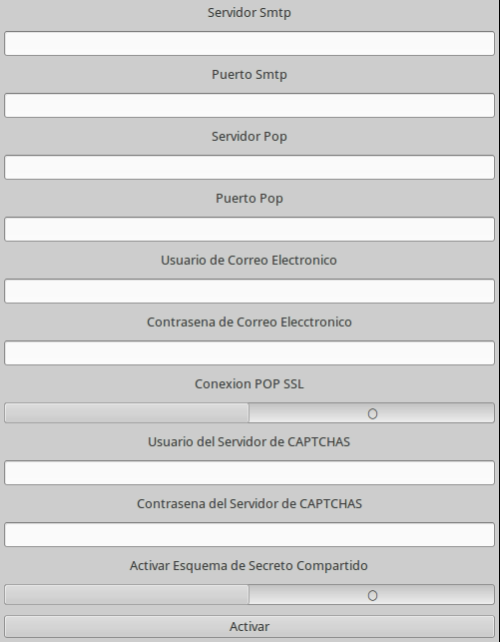
\includegraphics[width=10cm, height=10cm]{./images/VentanaConfig.png}
	\caption{Ventana de Configuración}
	\label{fig:6-10-1}
\end{figure}

Posteriormente se genero una interfaz gráfica principal para visualizar los mensajes de correos electrónicos y una segunda interfaz para la redacción de los mismos.

\begin{figure}[H]
\centering
	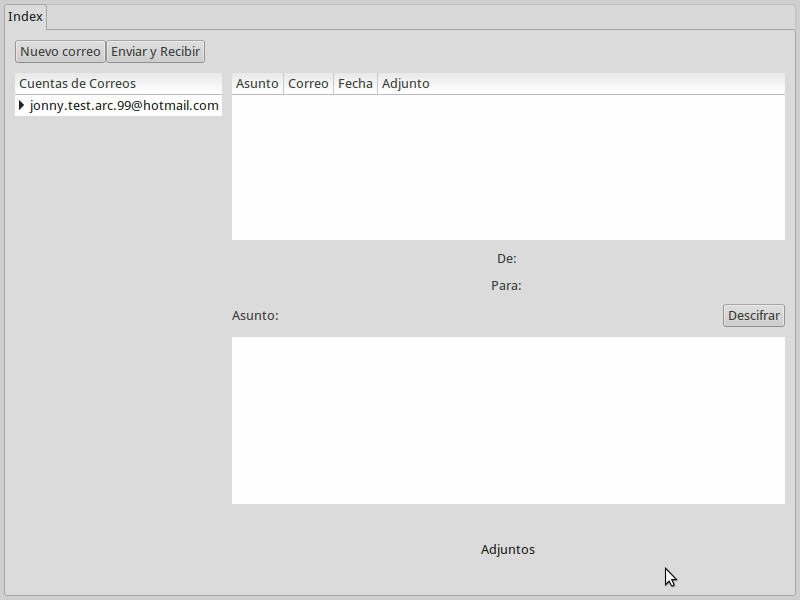
\includegraphics[width=15cm, height=10cm]{./images/VentanaPrincipal.png}
	\caption{Ventana Principal}
	\label{fig:6-10-2}
\end{figure}

La primera  interfaz, tambien llamada ventana principal, esta dividida en 3 parte una barra lateral, un listado y un visualizador de mensajes de correo electrónico. En la barra lateral encontramos las carpetas donde se almacenan los correo electrónicos, en el listado encontramos los mensajes de correos electrónicos que se han almacenado en la carpeta seleccionada de la barra lateral y por ultimo tenemos el visualizador de mensajes, el cual  despliega la dirección de correo del usuario que mando ese mensaje, los destinatarios a donde fue dirigido el mensaje y por ultimo el cuerpo del mensaje, ver figura n.

La segunda interfaz, también llamada ventana de envío de mensajes,  tiene un diseño simple para redactar los mensajes de correo electrónico, esta interfaz cuenta con 3 espacios, el primero es para escribir la dirección de correo donde se enviará el mensaje; el segundo espacio es para escribir el asunto que se adjunta al mensaje; y por último espacio es para la redacción del mismo, ver figura n.
\begin{figure}[H]
\centering
	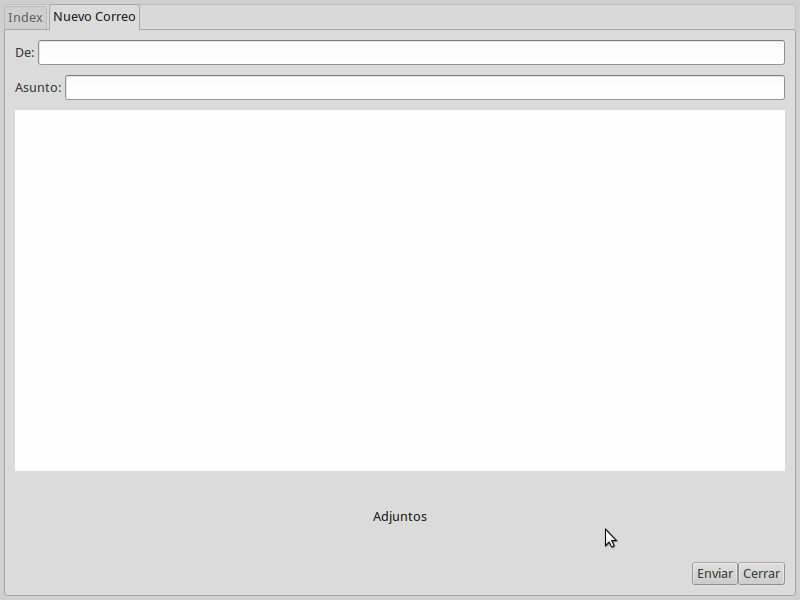
\includegraphics[width=15cm, height=10cm]{./images/VentanaNewCorreo.png}
	\caption{Ventana de Nuevo Correo}
	\label{fig:6-10-3}
\end{figure}
Una vez que se tienen las interfaces listas se procede a darles funcionalidad, para ello se llevan a cavo las siguientes actividades.
\begin{itemize}
 \item Cifrado de mensajes de correo electrónico por el protocolo P y P’: Esta actividad se inicia al redactar un correo electrónico en la ventana de envío de mensaje y pulsar el botón enviar. 
Lo primero que hace es toma la fecha actual de la computadora y la concatena con las dirección de correo destino y origen, a esta cadena generada  se le  obtiene un digesto MD5, el cual sera utilizado como firma para el mensaje de correo. Posteriormente se toma el mensaje redactado por el usuario y es enviado a la biblioteca de cifrado, prototipo 8, especificando el protocolo a usar. Esta biblioteca nos regresa el mensaje cifrado junto con la ruta de la imágenes CAPTCHAS que descifran el mensaje, Después se toma este mensaje cifrado y es concatenado con la firma generada anteriormente  y con una cabecera que nos indicara si el mensaje esta cifrado o no al momento de visualizarlo. Por ultimo se toman las direcciones de correo, origen y destino, el asunto redactado y el mensaje cifrado para generar un mensaje de correo electrónico y guardalo en la carpeta de salida, éste mensaje será enviado posteriormente por el protocolo SMTP al servidor de correos. Por ultimo esta actividad activa el envío de imágenes CAPTCHAS al servidor de CAPTCHAS.
 
 \item Envío de imágenes CAPTCHAS al servidor de CAPTCHAS: Esta actividad se inicia al momento de pulsar el botón “Enviar y Recibir” de la ventana principal o al termino del cifrado de mensajes de correo electrónico.
Esta actividad inicia tomando un listado de los mensajes de correo que se tienen pendientes de envío en la carpeta de salida y buscando los CAPTCHAS correspondientes a cada mensaje. Cada uno de estos CAPTCHAS son enviados al servidor junto con las direcciones de correo origen y destino, la firma del mensaje de correo y los datos de configuración del archivo JSON por medio de una petición HTTP. Por último, por cada CAPTCHA enviado exitosamente se envía su correspondiente mensaje al servidor de correo por el protocolo SMTP.
 \item Envío de mensajes por el protocolo SMTP: Esta actividad se inicia al momento de pulsar el botón “Enviar y Recibir” de la ventana principal o al termino de un envío exitoso de un CAPTCHA.
Para hacer el envío de un mensaje de correo electrónico se necesitan los datos de configuración que se tienen el el archivo JSON junto con el mensaje que se desea enviar. En caso de error el mensaje se almacena en la carpeta de salida.
 \item Descargar mensajes por POP3: Esta actividad se inicia al momento de pulsar el botón “Enviar y Recibir” de la ventana principal.
Para iniciar la descarga de los mensajes de correo electrónico se toman los datos básicos del archivo JSON para establecer comunicación con el servidor. Una vez establecida la conexión el servidor de correo electrónico nos dará uno a uno los mensajes y el cliente de correo electrónico guardará cada mensaje en un archivo txt en la carpeta de entrada.
 \item Descarga de imágenes CAPTCHAS del servidor de CAPTCHAS: Esta actividad se inicia al momento de pulsar el botón “Descifrar” de la ventana principal.
Para saber si el mensaje esta cifrado se busca en el cuerpo del mensaje la cabecera de cifrado de donde obtenemos la firma del mensaje. Con la firma del mensaje se buscan las imágenes de descifrado en la carpeta CAPTCHA, esta carpeta se crea con la instalación del prototipo, en caso de no encontrar las imágenes en la carpeta el cliente de correo hacer una petición HTTP al servidor de CAPTCHAS adjuntando la firma del mensaje, las direcciones de origen y la dirección destino.
El servidor contesta enviando la dirección URL de la imágenes de  donde  el cliente descarga las imágenes y las guarda en la carpeta CAPTCHA. Después de guardarlas, el cliente despliega la o las imágenes CAPTCHA en una ventana para que el usuario lo resuelva, esta ventana la llamaremos ventana de Descifrado. El despliegue de una o mas imágenes dependerá del protocolo que se haya utilizado para cifrar.
\begin{figure}[H]
\centering
	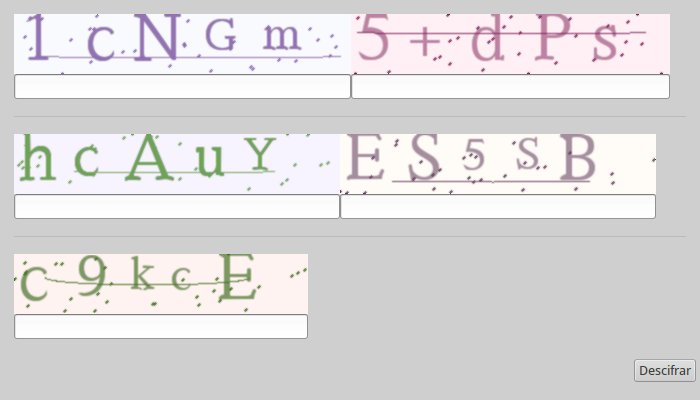
\includegraphics[width=15cm, height=7cm]{./images/VentanaMultiCAPTCHAS.png}
	\caption{Ventana Multi-CAPTCHAS}
	\label{fig:6-10-4}
\end{figure}
 \item Descifrado de mensajes de correo electrónico por el protocolo P y P’: Esta actividad se inicia al momento de pulsar el botón “Descifrar” de la ventana de Descifrado.
Una vez que el usuario resuelve los CAPTCHAS se toman las respuestas junto con el cuerpo del mensaje cifrado sin la cabecera de cifrado y se envían a la biblioteca de cifrado, prototipo 8, la cual nos regresa el texto descifrado. En caso de que los CAPTCHAS sean ingresados incorrectamente el texto regresado por la biblioteca sera ilegible y el cliente de correos lo detectara.

\begin{figure}[H]
\centering
	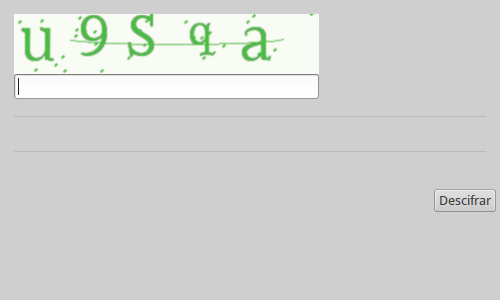
\includegraphics[width=10cm, height=5cm]{./images/VentanaCAPTCHA.png}
	\caption{Ventana CAPTCHAS}
	\label{fig:6-10-5}
\end{figure}

\end{itemize}
\textbf{Conclusión:}  El cliente de correo electrónico que se describió en este prototipo es completamente funcional y en conjunto con los prototipos 8 y 9 cumplen con el funcionamiento del esquema propuesto en este documento para implementar los protocolos P y P’ del esquema Díaz -Chakravorti. Para ver el codigo completo del prototipo 10 ver el anexo 5.
%\chapter{Pruebas}
En este capitulo se muestran los resultados de las pruebas realizadas sobre el prototipo 10. Las pruebas realizadas fueron de tiempo de respuesta y de trafico de información en la red.
\section{Prueba de rendimiento, Cifrado y Descifrado de un solo CAPTCHA}
En la figura \ref{fig:7-1} se muestra la relación de metodos que permiten el cifrado del mensaje y la generación de un solo CAPTCHA. El tiempo total que tarda en hacer todo el proceso es de 0.17s donde las funciones que tardan mas en realizar sus tareas son Ek\_din.crearCAPTCHA que se encarga de crear el CAPTCHA y la función Ek\_din.primoSig que calcula el numero primo mas cercano dependiendo del tamaño del CAPTCHA a realizar.\\\\
En la figura \ref{fig:7-2} se muestra la relación de metodos que permiten el descifrado del mensaje, este proceso es muy sencillo para un solo CAPTCHA ya que lo que introduce en usuario es lo que se canvierte en la clave de descifrado. El tiempo que tarda este proceso es de 0.004s.
\begin{figure}[H]
 \centering
 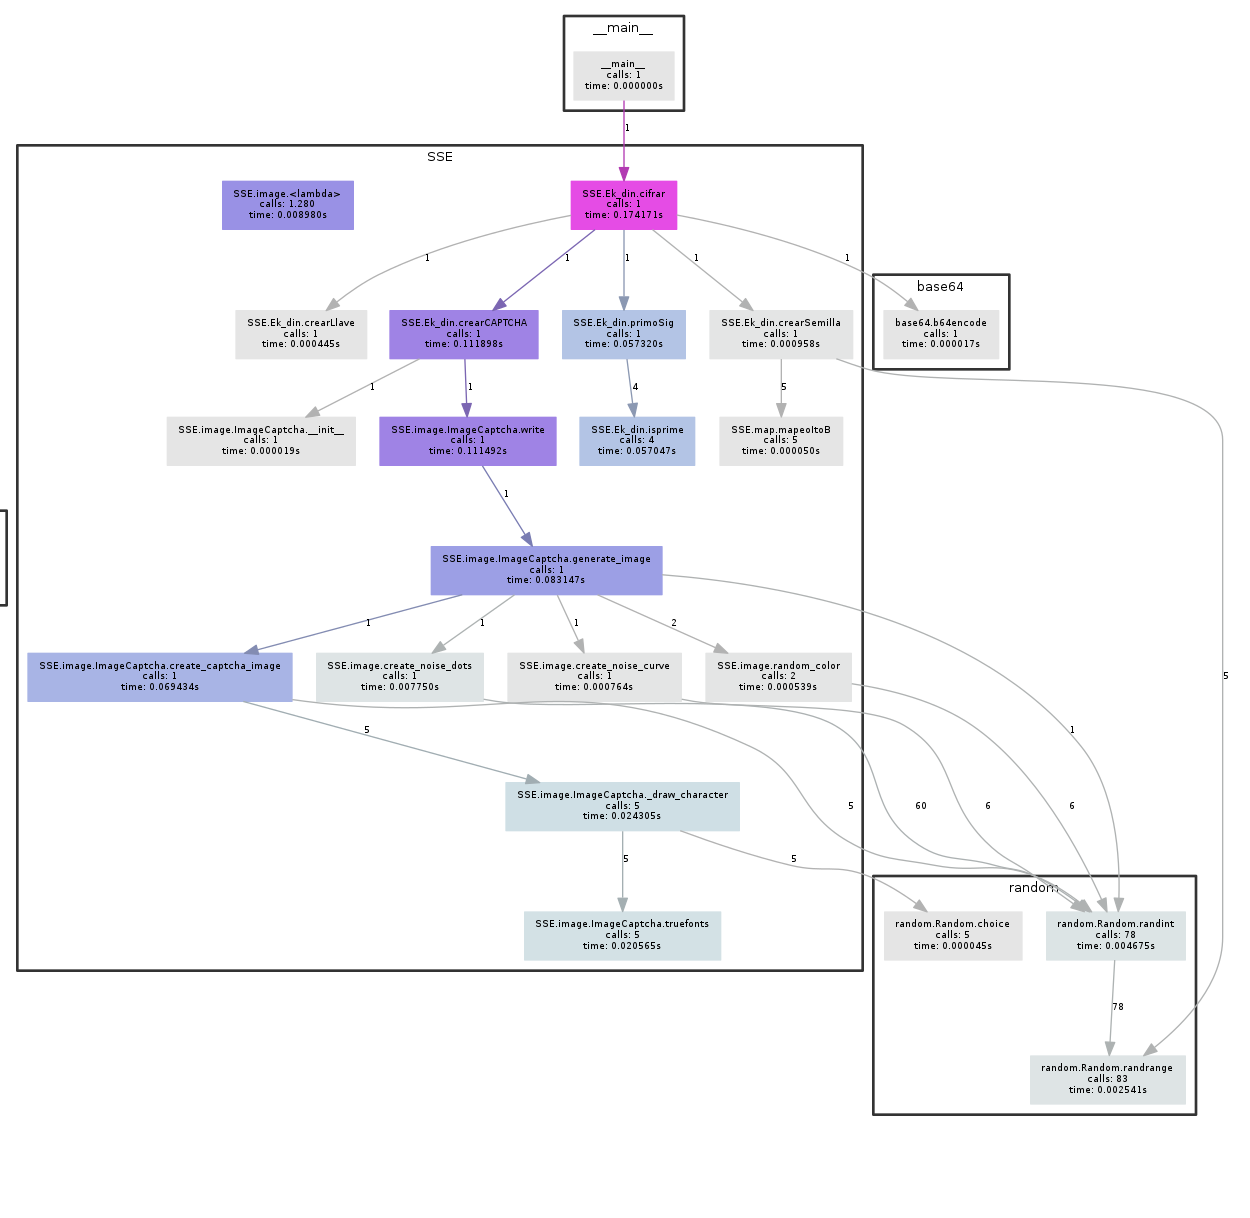
\includegraphics[height=7in]{./images/idda_unic.png}
		\caption{Rendimiento del esquema para un solo CAPTCHA}
		\label{fig:7-1}
\end{figure}

\begin{figure}[H]
 \centering
 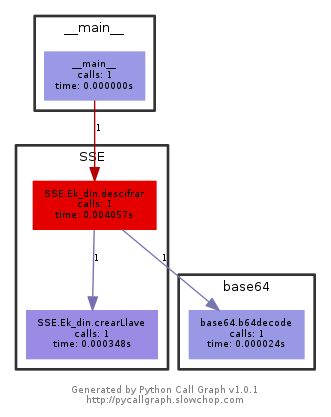
\includegraphics[height=6.3in]{./images/regreso_uni.png}
		\caption{Rendimiento del esquema para un solo CAPTCHA}
		\label{fig:7-2}
\end{figure}
\section{Prueba de rendimiento, Cifrado y Descifrado de multiples CAPTCHA's}
En la figura \ref{fig:7-3} se encuentra la relación de funciones que generan múltiples CAPTCHAS y cifran el mensaje, en este caso la llamada a funciones es mayor que para un solo CAPTCHA, se puede ver que al igual que en el esquema de un solo CAPTCHA las funciones que mas tardan son las de Ek\_din.crearCAPTCHA  y la función Ek\_din.primoSig dandonos un tiempo total para todo el proceso de 0.47s.\\\\
En la figura \ref{fig:7-4} se encuentra la relación de funciones que resuelve el algoritmo de secreto compartido y descifra el mensaje, este es mas elaborado que el descifrado para un solo CAPTCHA en este la función que mas tarda es Ek\_din.primoSig por el tamaño de numero que esta manejando, el tiempo total de termino de la tarea es 0.062s.
\begin{figure}[H]
 \raggedright
 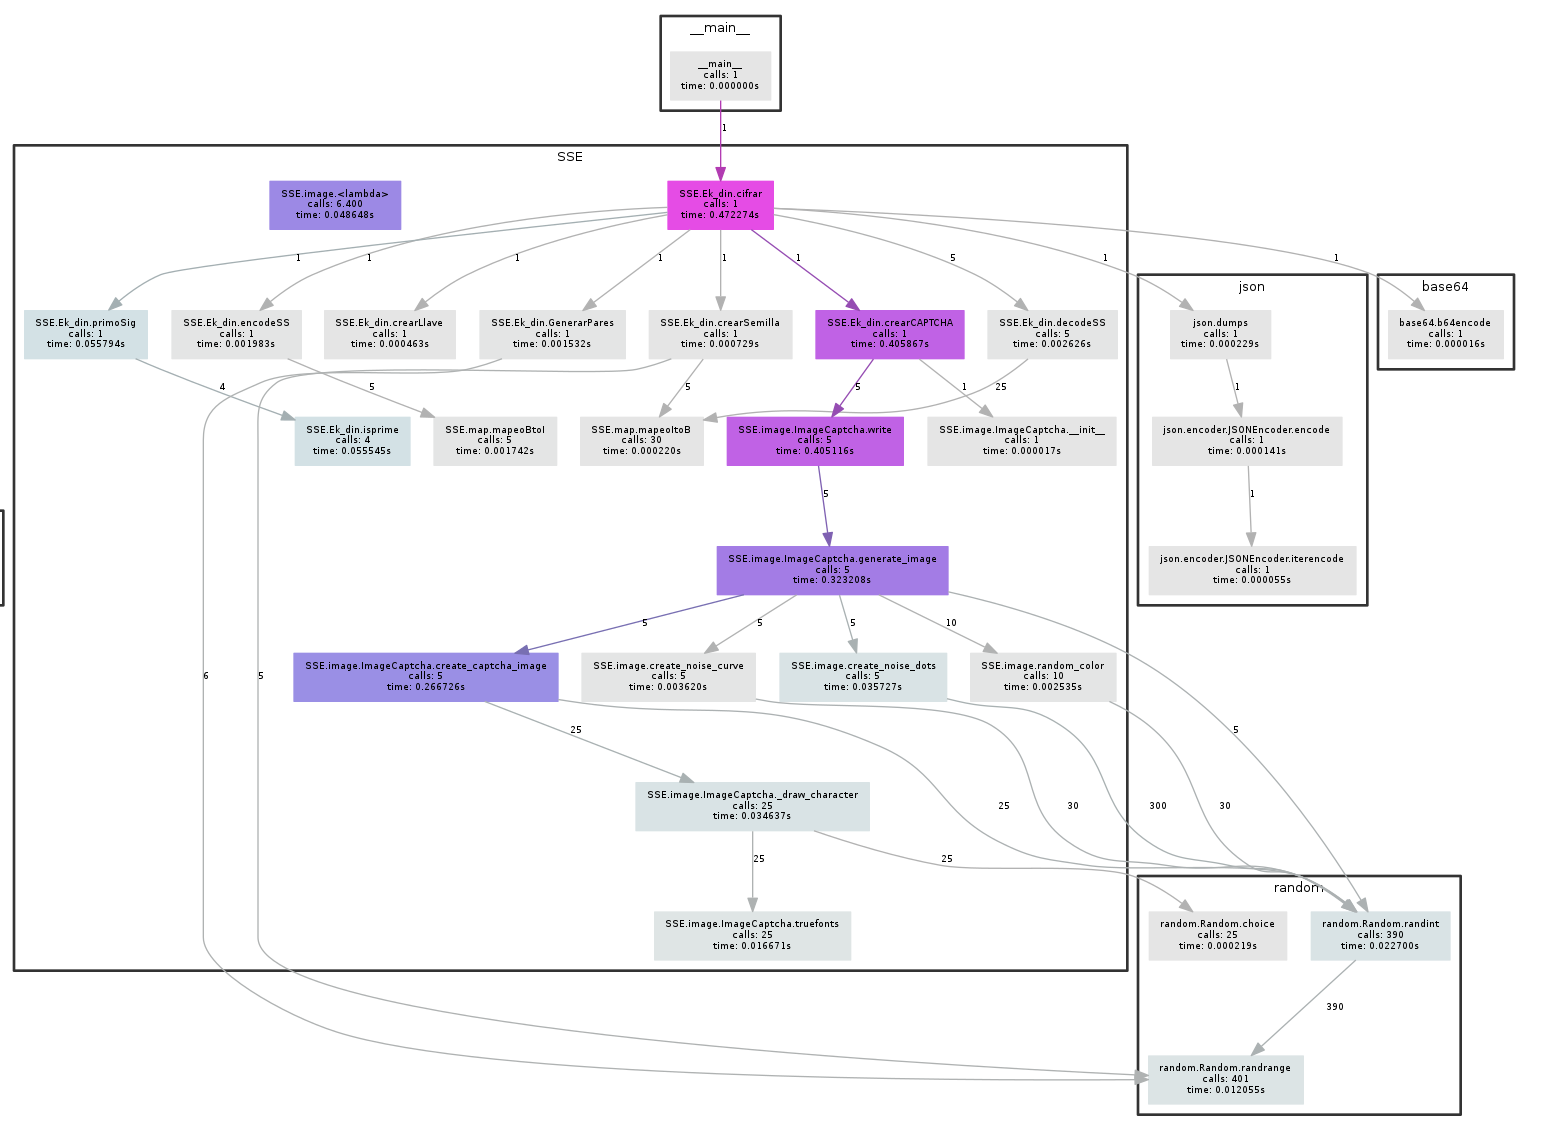
\includegraphics[height=5.5in]{./images/idda_multic.png}
		\caption{Rendimiento del esquema multiCAPTCHA}
		\label{fig:7-3}
\end{figure}
\begin{figure}[H]
 \raggedright
 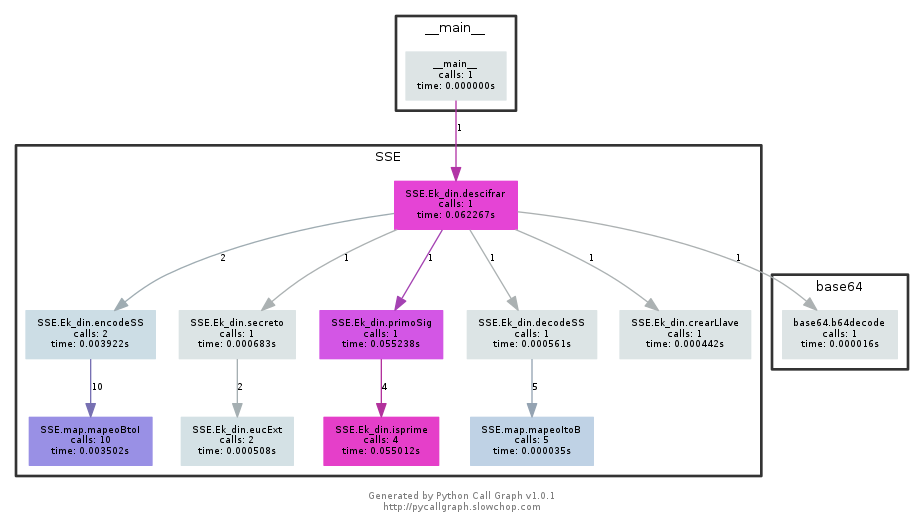
\includegraphics[height=4in]{./images/regraso_multi.png}
		\caption{Rendimiento del esquema multiCAPTCHA}
		\label{fig:7-4}
\end{figure}
%\chapter{Conclusiones y Trabajo a Futuro}
\section{Conclusiones}

En este documento se observa que el esquema de intercambio de clave y la implementación de los protocolos P y P’ del esquema Díaz – Chakraborty se lleva con éxito. Los cuales son implementados para el cifrado y descifrado de los mensajes de correo electrónico por medio de CAPTCHAS. \\

También se concluye que el esquema Díaz – Chakraborty es posible implementarse en los esquemas actuales de comunicación de correo electrónico de una manera trasparente al momento del envío y recepción de los correos electrónicos para el usuario.\\

El ataque de los adversarios clasificadores a la comunicación del correo electrónico no es explicada en su totalidad en los textos especializados del tema, solo se menciona que realizan una clasificación por medio de los mensajes en claro que obtiene. Sabemos que para realizar la conexión con los servidores de correo es necesaria una conexión POP3 y SMTP. Estas conexiones pueden proporcionar un canal seguro para transmitir por medio de los protocolos SSL o TLS. El tener una comunicación segura nos hace suponer que el ataque de los clasificadores no es por medio de la interseptación de los mensajes, si no que estos atacan directamente a los servidores de correo electrónico.



\section{Trabajo a futuro.}

Las líneas de trabajo que son sugeridas por los autores de este documento se describen a continuación.

La primera línea de trabajo que se sugiere al lector es la implementación del prototipo 8 en un cliente de correo electrónico comercial, ya sea un cliente de escritorio, como se hizo en este documento, un cliente de correos web o incluso un cliente de correo móvil.\\

Otra posible línea de trabajo tiene que ver con el intercambio de CAPTCHAS entre los usuarios para el descifrado de los mensajes de correo electrónico, en este documento se realizó en un esquema de intercambio basado en los servidores de claves públicas que se implementan en los protocolos PGP y GPG. Se sugiere mejorar la autenticación  de los usuarios en el servidor para la carga y descarga de los CAPTCHAS.\\

Por último, el prototipo 8 hace referencia mas a una biblioteca estándar que a una implementación solo orientada al correo electrónico ya que se tiene los protocolos P y P’ pueden utilizarse de manera separada. Se sugiere al lector utilizar estos protocolos para tratar resolver problemas de cifrado simétrico.
%\appendix
\chapter{Código fuente del prototipo 2}
\label{Anexos A}
A continuación se muestra el código fuente desarrollado en el prototipo 2.
\begin{itemize}
\item Archivo de cifrado (cifrado.py).
\end{itemize}

\begin{lstlisting}[frame=single]
 #! /usr/bin/env python
from Crypto.Hash import SHA256
from Crypto.Cipher import AES
from captcha.image import ImageCaptcha
import os
import random
hash = SHA256.new()
semilla=""
r=0
image = ImageCaptcha(fonts=['./fon/A.ttf', './fon/B.ttf'])
for i in range(5):
	r=random.randrange(100)
	semilla=semilla+chr(r)
	print str(i)+" "+str(r)+" "+chr(r)+" "+semilla
	
print semilla+"\n"

data = image.generate(semilla)
image.write(semilla, '/tmp/out.png')
image.write(semilla, 'out.png')

os.remove("/tmp/out.png")

hash.update(semilla)
otra=hash.digest()
llave = ""
print otra

for i  in range(16):
	llave=llave+otra[i]
	print str(i)+" "+otra[i]+" "+llave
\end{lstlisting}
\begin{lstlisting}[frame=single]
print "\n"
print llave
archy=open('llave.txt','w')
archy.write(semilla)
archy.close()
arc=open('cifrado.txt','w')
archi=open('1443750804.V805Idc01e2M920300.jonnytest:2,S','r')
obj = AES.new(llave, AES.MODE_ECB)
lineas=' '
c=0
while lineas!="": 
	c=c+1
	lineas=archi.read(16)
	
	if (((len(lineas))<16)and((len(lineas))>0)):
		c=16-(len(lineas))
		aux=lineas
		for i in range(c):
			aux=aux+" "
	else:
		aux=lineas
	
	ciphertext = obj.encrypt(aux)
	arc.write(ciphertext)
	print str(c) +"   " + lineas + "   "+str(len(lineas))+"   "
	+str(len(aux))+"   "+ciphertext
	

archi.close()
arc.close()



\end{lstlisting}
\begin{itemize}
\item Ventana de despliegue de CAPTCHAS (ventana.py)
\end{itemize}

\begin{lstlisting}[frame=single]
 #!/usr/bin/python
import Tkinter
import Image, ImageTk
imagenAnchuraMaxima=300
imagenAlturaMaxima=200
from Crypto.Hash import SHA256
from Crypto.Cipher import AES

import random
hash = SHA256.new()
# -*- coding: utf-8 -*-
\end{lstlisting}
\begin{lstlisting}[frame=single]
def funcion():

	a=e.get()
	print(a)
	hash.update(a)
	otra=hash.digest()
	llave = ""
	print otra
	for i  in range(16):	
		llave=llave+otra[i]
		print str(i)+" "+otra[i]+" "+llave
	
	print "\n"
	print llave
	archi=open('cifrado.txt','r')
	arc=open('descifrado.txt','w')
	obj = AES.new(llave, AES.MODE_ECB)
	lineas=' '
	c=0
	while lineas!="": 
		c=c+1
		lineas=archi.read(16)	
		if (((len(lineas))<16)and((len(lineas))>0)):
			c=16-(len(lineas))
			aux=lineas
			for i in range(c):
				aux=aux+" "
		else:
			aux=lineas
	
		ciphertext = obj.decrypt(aux)
		arc.write(ciphertext)
		print str(c) +"   " + lineas + "   "
		+str(len(lineas))+"   "+str(len(aux))+"   "
		+ciphertext
	archi.close()
	arc.close()
	root.quit()

# abrimos una imagen
img = Image.open('out.png')

img.thumbnail((imagenAnchuraMaxima,imagenAlturaMaxima)
, Image.ANTIALIAS)

root = Tkinter.Tk()
\end{lstlisting}
\begin{lstlisting}[frame=single]
root.title("Mostrar imagen")
# Convertimos la imagen a un objeto PhotoImage de Tkinter
tkimage = ImageTk.PhotoImage(img)

# Ponemos la imagen en un Lable dentro de la ventana
label=Tkinter.Label(root, image=tkimage, width=imagenAnchuraMaxima
, height=imagenAlturaMaxima).pack()

valor = ""
e = Tkinter.Entry(root)
e.pack()

buttonStart2=Tkinter.Button(root, text="Cerrar",
                            command=funcion).pack()
# Mostramos la ventana

root.mainloop()


\end{lstlisting}

\chapter{Código fuente del prototipo 8}
\label{Anexos B}
A continuación se muestra el código fuente desarrollado en el prototipo 8.

\begin{itemize}
\item Biblioteca de cifrado (Ek.py).
\end{itemize}

\begin{lstlisting}[frame=single]
from Crypto.Hash import SHA256
import os
import random
import base64
import json
from random import randrange
from map import mapeoBtoI
from map import mapeoItoB
from image import ImageCaptcha
from Crypto.Cipher import AES

def isprime(n): 

 n = abs(int(n)) 
 # 0 y 1 no son primos 
 if n < 2: 
  return False 
 # 2 es el unico primo par 
 if n == 2:  
  return True  
 # El resto de pares no son primos 
 if not n & 1:  
  return False 
 # El rango comienza en 3 y solo necesita subir 
 # hasta la raiz cuadrada de n  
 # para todos los impares 
 for x in range(3, int(n**0.5)+1, 2): 
  if n % x == 0: 
   return False 
 return True 
\end{lstlisting}
\begin{lstlisting}[frame=single]
def primoSig(num):
 buscar=True
 while buscar:
  if isprime(num):
   buscar=False
  else:
   num+=1
 return num
def crearSemilla(tam):
 r=0
 semilla=""
 for i in range(tam):
  r=random.randrange(64)
  semilla=semilla+str(mapeoItoB(r))
 return semilla

def crearLlave(semilla1):
 aux=""
 llave=""
 hash = SHA256.new()
 hash.update(semilla1)
 aux=hash.digest()
 llave = ""
 for i  in range(16):
  llave=llave+aux[i]
 return llave

def crearCAPTCHA(op,semilla2,asunto):
 imagen=""
 aux=""
 ax=[]
 xa=""
 s=[]
 c=0
 asunto=asunto.replace(" ","_")
 os.mkdir('./'+asunto+"",0755)
 image=ImageCaptcha(fonts=['./SSE/fon/A1.ttf','./SSE/fon/A1.ttf'])
 if (op==0):
  aux='./'+asunto+'/CAPTCHA00.png'
  image.write(semilla2, aux)
  return './'+asunto
 else:
  for x in semilla2:
   #print(x)
   aux='./'+asunto+'/CAPTCHA'+str(c)+'.png'
   xa='CAPTCHA'+str(c)+'.png'
\end{lstlisting}
\begin{lstlisting}[frame=single]
   ax.append(xa)
   s.append(ax)
   ax=[]
   image.write(x, aux)
   c=c+1
  return (s,'./'+asunto)

def encodeSS(strin):
 bina=""
 aux=""
 for i in range(len(strin)):
  aux=bin(mapeoBtoI(strin[i])).replace("0b","")
  if (len(aux)==6):
   bina=bina+aux
  else:
   while ((len(aux))<6):
    aux="0"+aux
   bina=bina+aux
 return int(str(bina),2)

def decodeSS(strr,w0):
 c=0
 s=""
 capt=""
 letras=[]
 z=bin(strr).replace("0b","")
 while (len(z)<(6*w0)):
  z="0"+z
 for i in z:
  if (c==5):
   c=0
   s=s+i
   letras.append(s)
   s=""
  else:
   c=c+1
   s=s+i
 for j in letras:
  capt=capt+mapeoItoB(int(str(j),2))
 return capt

def eucExt(a,b):
 r = [a,b]
 s = [1,0] 
 i = 1
 q = [[]]
\end{lstlisting}
\begin{lstlisting}[frame=single]
 while (r[i] != 0): 
  q = q + [r[i-1] // r[i]]
  r = r + [r[i-1] % r[i]]
  s = s + [s[i-1] - q[i]*s[i]]
  i = i+1
 return s[i-1]%b

def GenerarPares(p=7,w=5,t=2,k=0):
 pares =[]
 a = [k]
 for aux in range(0,w):
  print(aux)
  pares.append([randrange(p),0])
 print("X->")
 print(pares)
 for aux in range(1,t):
  print(aux)
  a.append(randrange(p))
 print("A->")
 print(a)
# for aux in range(0,w):
#  suma = k+(a[1]*pares[aux][0])
#  pares[aux][1] = suma%p
 for aux in pares:
  print("suma")
  suma = k
  print(suma)
  for aux2 in range(1,t):
   print("sin ecuacion")
   print(suma)
   suma = (suma+(a[aux2]*(aux[0]**aux2)))%p
   print("con ecuacion")
   print(suma)
  aux[1] =suma
 return pares

def secreto(pares,p):
 suma = 0
# print("pares")
# print(pares)
 for aux in pares:
#  print("par")
#  print(aux)
  ind = pares.index(aux)
#  print("index")
#  print(ind)
\end{lstlisting}
\begin{lstlisting}[frame=single]
  lis = pares[:ind] + pares[(ind+1):]
#  print("otros pares")
#  print(lis)
  num=1
  den=1
  for aux2 in lis:
#   print("numerodor")
   num = (num*(aux2[0])*-1)%p
#   print(num)
#   print("denominador")
   den = (den*((aux[0]-aux2[0])%p))%p
#   print(den)
#  print("Euclides")
  den = eucExt(den,p)
#  print(den)
  suma += (den*aux[1]*num)%p
#  print("suma")
#  print(suma)
 return suma%p

def cifrar(body,asunto1,op1=1,ta=5,w1=5,t1=2):
 ruta=""
 salida=""
 if t1>w1:
  salida=""
  ruta=None
  print("w1 < t1")
  return (salida,ruta)
 semilla3=crearSemilla(ta)
 num=0
 cap=[]
 zp=primoSig(2**(6*ta))
 disc={}
 #print(semilla3)
 if (op1==0):
  ruta=crearCAPTCHA(0,semilla3,asunto1)
 else:
  ruta=[]
  num=encodeSS(semilla3)
  pares=GenerarPares(zp,w1,t1,num)
  #print(pares)
  for x in pares:
   cap.append(decodeSS(x[1],w1))
  ruta=crearCAPTCHA(op1,cap,asunto1)
  num=0
  print(cap)
\end{lstlisting}
\begin{lstlisting}[frame=single]
  for x in pares:
   ruta[0][num].insert(0,x[0])
   num=num+1
  for i in ruta[0]:
   disc[i[1]]=i[0]
  print(ruta)
  lista=open(ruta[1]+"/lista.json","w") 
  lista.write(json.dumps(disc))
  lista.close
 k=crearLlave(semilla3)
 obj = AES.new(k, AES.MODE_ECB)
 salida=""
 ax=0
 c=0
 strr=""
 #print len(body)
 while (ax < len(body)):
  while (c<16):
   if (ax>=len(body)):
    strr=strr+" "
   else:
    strr=strr+body[ax]
   c=c+1
   ax=ax+1
   #print str(c) +" " + str(ax) 
  c=0
  #print strr
  ciphertext = obj.encrypt(strr)
  salida=salida+ciphertext
  strr=""
 salida = base64.b64encode(salida)
 return (salida,ruta)

def descifrar(body1,capt1,op2):
 aux=[]
 ax=0
 pares=[]
 zp=0
 
 if (op2==0):
  k=crearLlave(capt1)
 else:
  w=len(capt1[0][1])
  zp=primoSig(2**(6*(len(capt1[0][1]))))
  for x in capt1:
   aux=x
\end{lstlisting}
\begin{lstlisting}[frame=single]
   aux[1]=encodeSS(x[1])
   pares.append(aux) 
  #print(pares)
  ax=secreto(pares,zp)
  #print(ax)
  semilla4=decodeSS(ax,w)
  #print(semilla4)
  k=crearLlave(semilla4)
  #print(k)
 obj = AES.new(k, AES.MODE_ECB)
 salida=""
 ax=0
 c=0
 strr=""
 #print len(body1)
 body1 = base64.b64decode(body1)
 while (ax < len(body1)):
  while (c<16):
   if (ax>=len(body1)):
    strr=strr+" "
   else:
    strr=strr+body1[ax]
   c=c+1
   ax=ax+1
   #print str(c) +" " + str(ax) 
  c=0
  #print strr
  ciphertext = obj.decrypt(strr)
  salida=salida+ciphertext
  strr=""
 return salida
\end{lstlisting}

\begin{itemize}
\item Generador de imágenes CAPTCHAS (imagen.py).
\end{itemize}

\begin{lstlisting}[frame=single]
# coding: utf-8

import os
import random
from PIL import Image
from PIL import ImageFilter
from PIL.ImageDraw import Draw
from PIL.ImageFont import truetype
try:
 from cStringIO import StringIO as BytesIO
except ImportError:
 from io import BytesIO
\end{lstlisting}
\begin{lstlisting}[frame=single]
try:
 from wheezy.captcha import image as wheezy_captcha
except ImportError:
 wheezy_captcha = None
DATA_DIR = os.path.join(os.path.abspath(os.path.dirname(__file__))
                        , 'data')
DEFAULT_FONTS = [os.path.join(DATA_DIR, 'DroidSansMono.ttf')]

if wheezy_captcha:
 __all__ = ['ImageCaptcha', 'WheezyCaptcha']
else:
 __all__ = ['ImageCaptcha']

class _Captcha(object):
 def generate(self, chars, format='png'):
  im = self.generate_image(chars)
  out = BytesIO()
  im.save(out, format=format)
  out.seek(0)
  return out

 def write(self, chars, output, format='png'):
  im = self.generate_image(chars)
  return im.save(output, format=format)

class WheezyCaptcha(_Captcha):
 def __init__(self, width=200, height=75, fonts=None):
  self._width = width
  self._height = height
  self._fonts = fonts or DEFAULT_FONTS

 def generate_image(self, chars):
  text_drawings = [wheezy_captcha.warp(),wheezy_captcha.rotate(),
                   wheezy_captcha.offset(),]
  fn = wheezy_captcha.captcha(
   drawings=[
    wheezy_captcha.background(),
    wheezy_captcha.text(fonts=self._fonts, drawings=text_drawings),
    wheezy_captcha.curve(),
    wheezy_captcha.noise(),
    wheezy_captcha.smooth(),],
   width=self._width,
   height=self._height,
  )
  
  return fn(chars)
\end{lstlisting}
\begin{lstlisting}[frame=single]
class ImageCaptcha(_Captcha):

 def __init__(self,width=160,height=60,fonts=None,font_sizes=None):
 
  self._width = width
  self._height = height
  self._fonts = fonts or DEFAULT_FONTS
  self._font_sizes = font_sizes or (46, 58, 68)
  self._truefonts = []

 @property
 def truefonts(self):
 
  if self._truefonts:
   return self._truefonts
  self._truefonts = tuple([
   truetype(n, s)
   for n in self._fonts
   for s in self._font_sizes
  ])
  return self._truefonts

 @staticmethod
 def create_noise_curve(image, color):
 
  w, h = image.size
  x1 = random.randint(0, int(w / 5))
  x2 = random.randint(w - int(w / 5), w)
  y1 = random.randint(h / 5, h - int(h / 5))
  y2 = random.randint(y1, h - int(h / 5))
  points = [(x1, y1), (x2, y2)]
  end = random.randint(160, 200)
  start = random.randint(0, 20)
  Draw(image).arc(points, start, end, fill=color)
  return image

 @staticmethod
 def create_noise_dots(image, color, width=3, number=30):
  draw = Draw(image)
  w, h = image.size
  while number:
   x1 = random.randint(0, w)
   y1 = random.randint(0, h)
   draw.line(((x1, y1), (x1 - 1, y1 - 1)), fill=color, width=width)
   number -= 1
  return image
\end{lstlisting}
\begin{lstlisting}[frame=single]
 def create_captcha_image(self, chars, color, background):

  image = Image.new('RGB', (self._width, self._height), background)
  draw = Draw(image)

  def _draw_character(c):
   font = random.choice(self.truefonts)
   w, h = draw.textsize(c, font=font)

   #dx = random.randint(4, 6)
   #dy = random.randint(4, 8)
   im = Image.new('RGBA', (w+30 , h+30 ))
   Draw(im).text((0, 0), c, font=font, fill=color)

   # rotate
   #im = im.crop(im.getbbox())
   #im = im.rotate(random.uniform(-30, 30),Image.BILINEAR,expand=1)
   # warp
   #dx = w * random.uniform(0.1, 0.3)
   #dy = h * random.uniform(0.2, 0.3)
   #x1 = int(random.uniform(-dx, dx))
   #y1 = int(random.uniform(-dy, dy))
   #x2 = int(random.uniform(-dx, dx))
   #y2 = int(random.uniform(-dy, dy))
   #w2 = w + abs(x1) + abs(x2)
   #h2 = h + abs(y1) + abs(y2)
   #data = (
   # x1, y1,
   # -x1, h2 - y2,
   # w2 + x2, h2 + y2,
   # w2 - x2, -y1,
   #)
   #im = im.resize((w2, h2))
   #im = im.transform((w, h), Image.QUAD, data)
   return im
   
  images = []
  for c in chars:
   images.append(_draw_character(c))

  text_width = sum([im.size[0] for im in images])
  width = max(text_width, self._width)
  image = image.resize((width, self._height))
  average = int(text_width / len(chars))
  rand = int(0.25 * average)
  offset = int(average * 0.1)
\end{lstlisting}
\begin{lstlisting}[frame=single]
  for im in images:
   w, h = im.size
   mask = im.convert('L').point(lambda i: i * 1.97)
   image.paste(im, (offset, int((self._height - h) / 2)), mask)
   offset = offset + w + random.randint(-rand, 0)

  return image

 def generate_image(self, chars):
  """Generate the image of the given characters.

  :param chars: text to be generated.
  """
  background = random_color(238, 255)
  color = random_color(0, 200, random.randint(220, 255))
  im = self.create_captcha_image(chars, color, background)
  self.create_noise_dots(im, color)
  self.create_noise_curve(im, color)
  im = im.filter(ImageFilter.SMOOTH)
  return im


def random_color(start, end, opacity=None):
 red = random.randint(start, end)
 green = random.randint(start, end)
 blue = random.randint(start, end)
 if opacity is None:
  return (red, green, blue)
 return (red, green, blue, opacity)
\end{lstlisting}
\begin{itemize}
\item Empaquetado de imágenes CAPTCHA (empaquetar.py).
\end{itemize}

\begin{lstlisting}[frame=single]
from Ek_din import cifrar
from subprocess import call
import types
import os
from os import path

def listFiles(folder):
 return [d for d in os.listdir(folder) 
         if path.isfile(path.join(folder, d))]

def empaquetar(body,asunto,op):
 s=cifrar(body,asunto,op)
 asunto=asunto.replace(" ","_")
 disc={}
\end{lstlisting}
\begin{lstlisting}[frame=single]
 #print(s[1])
 ass=asunto+".zip"
 if type(s[1])==types.StringType:
  zi=call("zip -r "+ass+" "+s[1], shell=True)
  mv=call("mv ./"+ass+" ./CAPTCHAS", shell=True)
  rmm=call("rm -rf "+s[1], shell=True)
  return (s[0],"./CAPTCHAS/"+ass)
 else:
  zi=call("zip -r "+ass+" "+s[1][1], shell=True)
  mv=call("mv ./"+ass+" ./CAPTCHAS", shell=True)
  rmm=call("rm -rf "+s[1][1], shell=True)
  return (s[0],"./CAPTCHAS/"+ass)
\end{lstlisting}

\chapter{Código fuente del prototipo 9}
\label{Anexos C}

A continuación se muestra el código fuente desarrollado en el prototipo 9.
\begin{itemize}
\item Estructura de la base de datos (script.sql).
\end{itemize}

 \begin{lstlisting}[frame=single]
 CREATE TABLE IF NOT EXISTS `Mensaje` (
  `firma_digital` varchar(255) CHARACTER SET utf8 NOT NULL,
  `correo_destino` varchar(50) CHARACTER SET utf8 NOT NULL,
  `ruta_archivo` varchar(255) CHARACTER SET utf8 NOT NULL,
  `correo_electronico` varchar(50) CHARACTER SET utf8 NOT NULL,
  PRIMARY KEY (`correo_destino`,`firma_digital`)
 ) ENGINE=MyISAM DEFAULT CHARSET=utf8 COLLATE=utf8_unicode_ci;

 CREATE TABLE IF NOT EXISTS `Usuario` (
  `correo_electronico` varchar(50) CHARACTER SET utf8 NOT NULL,
  `nombre` varchar(150) CHARACTER SET utf8 NOT NULL,
  `contrasena` varchar(20) COLLATE utf8_unicode_ci NOT NULL
 ) ENGINE=MyISAM DEFAULT CHARSET=utf8 COLLATE=utf8_unicode_ci;
 \end{lstlisting}
\begin{itemize}
\item Alta de usuario en el servidor de CAPTCHAS (AltaUsuario.php).
\end{itemize}

 \begin{lstlisting}[frame=single]
 <html>
 <head>
  <title>Alta de usuario</title> 
 </head>

 <body>
<?php
$usuario = trim($_POST["nombre"]);
$contra = trim($_POST["contrasena"]);
$correo = trim($_POST["correo_electronico"]);
if (empty($usuario)){
 echo '<p name="respuesta">0</p>';
}elseif (empty($contra)) {
 echo '<p name="respuesta">1</p>';
\end{lstlisting}
\begin{lstlisting}[frame=single]
}elseif (empty($correo)) {
 echo '<p name="respuesta">2</p>';
}else{
 $enlace = new mysqli('mysql.hostinger.mx', 'u715698692_corre',
                      'correocifrado','u715698692_corre');
 if($enlace->connect_errno){
  echo '<p name="respuesta">3</p>';
  die("Error en conexion");
 }

 if (!file_exists("./Usuarios/".$correo)) {
  mkdir("./Usuarios/".$correo);
 }

 $query = "SELECT nombre FROM Usuario 
            WHERE correo_electronico like '$correo'";
 $result = $enlace->query($query);
 $aux = $result->num_rows;
 if($aux == 1){
  echo '<p name="respuesta">5</p>';
  $enlace->close();
 }else{
  $result->free();
  if($enlace->query("INSERT INTO `Usuario`
  (`correo_electronico`, `nombre`, `contrasena`) 
  VALUES 
  ('".$correo."','".$usuario."','".$contra."')") === TRUE){
   echo '<p name="respuesta">5</p>';
   $enlace->close();
  }else{
   echo '<p name="respuesta">6</p>';
   $enlace->close();
  }
 }
}
?>
 </body>
</html>
 \end{lstlisting}

\begin{itemize}
\item Carga de imágenes CAPTCHAS en el servidor (AltaMensage.php).
\end{itemize}

 \begin{lstlisting}[frame=single]
 <html>
 <head>
  <title>Alta de Mensaje</title> 
 </head>
\end{lstlisting}
\begin{lstlisting}[frame=single]
 <body>
<?php
$usuario = trim($_POST["nombre"]);
$contra = trim($_POST["contrasena"]);
$correo = trim($_POST["correo_electronico"]);
$firma = trim($_POST["firma"]);
$correo_des = trim($_POST["correo_destino"]);

if (empty($usuario)){
 echo '<p name="respuesta">0</p>';
 die();
}elseif (empty($contra)) {
 echo '<p name="respuesta">1</p>';
 die();
}elseif (empty($correo)) {
 echo '<p name="respuesta">2</p>';
 die();
}elseif (empty($firma)) {
 echo '<p name="respuesta">3</p>';
 die();
}elseif (empty($correo_des)) {
 echo '<p name="respuesta">4</p>';
 die();
}elseif (!is_uploaded_file($_FILES["archivo"]["tmp_name"])){
 echo '<p name="respuesta">6</p>';
 die();
}else{
 $enlace = new mysqli('mysql.hostinger.mx', 'u715698692_corre', 
           'correocifrado','u715698692_corre');
 if($enlace->connect_errno){
  echo '<p name="respuesta">7</p>';
  die("Error en conexion");
 }
 $query = "SELECT nombre, contrasena 
           FROM Usuario 
           WHERE Correo_Electronico like '$correo' ";
 $result = $enlace->query($query);
 $aux = $result->num_rows;
 
 if($aux >0){
  $row = $result->fetch_array(MYSQLI_ASSOC);
 }else{
  echo '<p name="respuesta">11</p>';
  $enlace->close();
  die("Error de autenticacion");
 }
\end{lstlisting}
\begin{lstlisting}[frame=single]
 if(!(strcmp($row["nombre"],$usuario) == 0)){
  echo '<p name="respuesta">8</p>';
  $enlace->close();
  die("Error de autenticacion 1");
 }
 if (!(strcmp($row["contrasena"],$contra) == 0)) {
  echo '<p name="respuesta">8</p>';
  $enlace->close();
  die("Error de autenticacion 2");
 }
 $result->free();
 if(strcmp($_FILES['archivo']['type'], "application/zip")==0){
  $file= sha1($correo_des.$firma.$correo).".zip";
  $ruta=join(DIRECTORY_SEPARATOR,array("./Usuarios",
        $correo,$file));
  $query = "SELECT ruta_archivo 
            FROM Mensaje 
            WHERE Correo_Electronico like '$correo' 
            and firma_digital like '$firma' 
            and correo_destino like '$correo_des'";
  $result = $enlace->query($query);
  $aux = $result->num_rows;

  if($aux >0){
   echo '<p name="respuesta">12</p>';
   $enlace->close();
   die("Error de autenticacion");
  }else{
   $result->free();
   if (!file_exists($ruta)) {
    move_uploaded_file($_FILES['archivo']['tmp_name'], $ruta);
    echo "<pre>";
    print_r($ruta);
    if($enlace->query("INSERT INTO `Mensaje`
    (`firma_digital`, `correo_destino`, `ruta_archivo`, 
    `correo_electronico`) 
    VALUES ('".$firma."','".$correo_des."',
    '".$ruta."','".$correo."')") === TRUE){
     echo '<p name="respuesta">5</p>';
     $enlace->close();
    }else{
     echo '<p name="respuesta">9</p>';
     $enlace->close();
    }
   }else{
    echo '<p name="respuesta">13</p>';
\end{lstlisting}
\begin{lstlisting}[frame=single]
    $enlace->close();
    die("Error de autenticacion");
   }
  }
 }else{
  echo '<p name="respuesta">10</p>';
  $enlace->close();
 }

}
?>
 </body>
</html>
 \end{lstlisting}
\begin{itemize}
\item Descarga de imágenes CPATCHAS del servidor (BusquedaArchivo.php).
\end{itemize}

 \begin{lstlisting}[frame=single]
 <html>
 <head>
  <title>Busqueda de Archivos</title> 
 </head>

 <body>
<?php

$correo = trim($_POST["correo_electronico"]);
$firma = trim($_POST["firma"]);
$correo_des = trim($_POST["correo_destino"]);

if (empty($correo)) {
 echo '<p name="respuesta">0</p>';
 die();
}elseif (empty($firma)) {
 echo '<p name="respuesta">1</p>';
 die();
}elseif (empty($correo_des)) {
 echo '<p name="respuesta">2</p>';
 die();
}else{

 $enlace = new mysqli('mysql.hostinger.mx', 'u715698692_corre',
           'correocifrado','u715698692_corre');
 if($enlace->connect_errno){
  echo '<p name="respuesta">7</p>';
  die("Error en conexion");

 }
\end{lstlisting}
\begin{lstlisting}[frame=single]
 $query = "SELECT ruta_archivo 
           FROM Mensaje 
           WHERE Correo_Electronico like '$correo' 
           and firma_digital like '$firma' 
           and correo_destino like '$correo_des'";
 $result = $enlace->query($query);
 $aux = $result->num_rows;
 if($aux == 1){
  $row = $result->fetch_array(MYSQLI_ASSOC);
  $ruta = "http://correocifrado.esy.es".$row["ruta_archivo"];
  echo '<p name="respuesta">'.$ruta.'</p>';
  $enlace->close();
 }else{
  echo '<p name="respuesta">4</p>';
  $enlace->close();
  die("Error de autenticacion");
 }

}
?>
 </body>
</html>
 \end{lstlisting}

\chapter{Intalación de biblioteca GTK+ 3 y entorno gráfico GNOME 3}
\label{Anexos D}

A continuación se muestra los pasos a seguir para la intalación de las bibliotecas GTK3+ y el entorno grafico GNOME 3.

\section{Instalación del entorno gráfico GNOME 3.}


La instalación del entorno gráfico GNOME 3 se realizo en un sistema operativo XUBUNTU 15.1 y XUBUNTU 14.1. A continuación se explica los pasos a seguir para la instalación de este entorno gráfico.
\begin{itemize}
\item Se abre una terminal del sistema operativo.
\item Se ingresan los siguientes comandos a la terminal para instalar los repositorios de descarga.
\begin{lstlisting}
sudo add-apt-repository ppa:gnome3-team/gnome3
sudo add-apt-repository ppa:gnome3-team/gnome3-staging
\end{lstlisting}

\item Posteriormente se ingresa el siguiente comando a la terminal para actualizar los repositorios de descarga.
\begin{lstlisting}
sudo apt-get update
\end{lstlisting}

\item Una vez terminada la actualización se  ingresa este último comando para terminar con la instalación del entorno gráfico GNOME 3.
\begin{lstlisting}
sudo apt-get dist-upgrade
\end{lstlisting}
Una vez que la instalación termine se reinicia el equipo para activar el entorno gráfico GNOME 3.

\end{itemize}
\pagebreak
\section{Instalación de la biblioteca gráfica GTK+ 3.}

La instalación del biblioteca gráfica GTK+ 3 se realizo en un sistema operativo XUBUNTU 15.1 y XUBUNTU 14.1 siguiendo  los tutoriales proporcionados por la pagina de Python GTK+ 3 Tutorial y GNOME developer.
Uno de los requisitos previos para la instalación de GTK+ 3 es la instalación de JHBuild la cual se instalo siguiendo el tutorial de GNOME developer encontrado en la siguiente pagina web:\\
\url{https://developer.gnome.org/jhbuild/unstable/getting-started.html.es}\\

Después de la instalación de JHBuild se prosiguió con la instalación de la biblioteca gráfica GTK+ 3. A continuación se presentan los pasos a seguir para la instalación de de la biblioteca.
\begin{itemize}
\item Se abre una terminal del sistema operativo.
\item Se ingresan los siguientes comandos.
\begin{lstlisting}
$ jhbuild build pygobject
$ jhbuild build gtk+
$ jhbuild shell
\end{lstlisting}
\end{itemize}

\chapter{Código fuente del prototipo 10}
\label{Anexos E}

A continuación se muestra el código fuente desarrollado en el prototipo 10.
\begin{itemize}
\item Archivo de configuración JSON config.json).
\end{itemize}

\begin{lstlisting}[frame=single]
{
certfile: "./Seguridad/server2048.pem",
passwdSSE: "12345678",
passwd: "360_live",
portSmtp: "587",
portPop: "995",
ssl: true,
hostSmtp: "smtp-mail.outlook.com",
user: "jonny.test.arc.99@hotmail.com",
SSE: false,
nombre: "jonathan arcos",
hostPop: "pop3.live.com",
keyfile: "./Seguridad/server2048.key",
delete: 0
}
\end{lstlisting}
\begin{itemize}
\item Interfaz gráfica del cliente de correo electrónico (setup.py).
\end{itemize}

\begin{lstlisting}[frame=single]
import gi
import os
import email
import json
import SSE
import re
import captchas
import http
import logging

gi.require_version('Gtk', '3.0')
from gi.repository import Gtk, Gio
\end{lstlisting}
\begin{lstlisting}[frame=single]
from smtp2 import datosPrincipales
from smtp2 import validarSmtp
from listarCorreos import listaCorreosView
from listarCorreos import contarCorreo
from listarCorreos import body
from pop3 import conexionPop3
from pop3 import validarPop
from envios import envios
from salidaSmtp import salida

path = './Usuarios'

def listdirs(folder):
 return [d for d in os.listdir(folder) 
        if os.path.isdir(os.path.join(folder, d))]

def listFiles(folder):
 return [d for d in os.listdir(folder) 
        if os.path.isfile(os.path.join(folder, d))]

class MyWindow(Gtk.Window):

 user=listdirs(path)
 selectCarpeta=None
 selectUsuario=None
 config={}

 def __init__(self,config):
  self.config = config
  Gtk.Window.__init__(self, title="Cliente de Correos")
  self.set_border_width(4)
  self.set_default_size(800, 600)

  self.notebook = Gtk.Notebook()
  self.add(self.notebook)

  self.page = self.newPage()
  self.page.set_border_width(10)
  self.notebook.append_page(self.page, Gtk.Label('Index'))

 def visorCorreo(self):
  vistaCorre = Gtk.Box(orientation=Gtk.Orientation.VERTICAL, 
                       spacing=10)
  self.emisor = Gtk.Label("De: ")
  self.emisor.set_justify(Gtk.Justification.LEFT)
  self.destinatorio = Gtk.Label("Para: ")
\end{lstlisting}
\begin{lstlisting}[frame=single]
  self.destinatorio.set_justify(Gtk.Justification.LEFT)
  self.asunto = Gtk.Label("Asunto: ")
  self.asunto.set_justify(Gtk.Justification.LEFT)
  descifrado= Gtk.Button(label="Descifrar")
  descifrado.connect("clicked", self.descifrarBody)
  box1 = Gtk.VBox(False,10)
  box1.pack_start(self.emisor,True,True,0)
  box1.pack_end(self.destinatorio,False,True,0)
  box2 = Gtk.HBox(False,0)
  box2.pack_start(self.asunto,False, False, 0)
  box2.pack_end(descifrado,False,False,0)
  self.cuerpo = Gtk.TextView()
  self.cuerpo.set_wrap_mode(Gtk.WrapMode.WORD)
  self.cuerpo.set_editable(False)
  scrol = Gtk.ScrolledWindow()
  scrol.set_policy(Gtk.PolicyType.AUTOMATIC, 
                   Gtk.PolicyType.AUTOMATIC)
  scrol.set_vexpand(True)
  scrol.add(self.cuerpo)
  vistaCorre.add(box1)
  vistaCorre.add(box2)
  vistaCorre.add(scrol)
  return vistaCorre

 def visorCorreoNuevo(self):
  vistaCorre = Gtk.Box(orientation=Gtk.Orientation.VERTICAL, 
                       spacing=10)
                       
  newDest = Gtk.Entry(name="Destino")
  newDest.set_editable(True)
  newAsunto = Gtk.Entry(name="Asunto")
  newAsunto.set_editable(True)
  destinatorio = Gtk.Label("De: ")
  destinatorio.set_justify(Gtk.Justification.LEFT)
  asunto = Gtk.Label("Asunto: ")
  asunto.set_justify(Gtk.Justification.LEFT)
  Cerrar = Gtk.Button(label="Cerrar")
  Cerrar.connect("clicked", self.cerrarPagina)
  Enviar = Gtk.Button(label="Enviar")
  Enviar.connect("clicked", self.enviarMensage)
  box1 = Gtk.HBox(False,0)
  box1.pack_start(destinatorio,False,False,0)
  box1.pack_start(newDest,True,True,0)  
  box2 = Gtk.HBox(False,0)
  box2.pack_start(asunto,False, False, 0)
  box2.pack_start(newAsunto,True, True, 0)
\end{lstlisting}
\begin{lstlisting}[frame=single]
  box3 = Gtk.HBox(False,0)
  box3.pack_end(Cerrar,False, False, 0)
  box3.pack_end(Enviar,False, False, 0)

  cuerpo = Gtk.TextView(name="cuerpo")
  cuerpo.set_wrap_mode(Gtk.WrapMode.WORD)
  #WRAP_WORD
  scrol = Gtk.ScrolledWindow()
  scrol.set_policy(Gtk.PolicyType.AUTOMATIC, 
                   Gtk.PolicyType.AUTOMATIC)
  scrol.set_vexpand(True)
  scrol.add(cuerpo)
  vistaCorre.add(box1)
  vistaCorre.add(box2)
  vistaCorre.add(scrol)
  vistaCorre.add(box3)
  return vistaCorre

 def cerrarPagina(self,button):
  print("cerrarPagina")
  page=self.notebook.get_current_page()
  self.notebook.remove_page(page)
  self.notebook.show_all()

 def enviarMensage(self,button):
  print("enviarMensage")
  page=self.notebook.get_current_page()
  contenedor = self.notebook.get_nth_page(page)
  asunto = ""
  destino = ""
  cuerpo = ""
  for c in contenedor.get_children():
    for x in c.get_children():
     if isinstance(x,Gtk.Entry):
      if x.get_name() == "Destino":
       destino = x.get_text()
      elif x.get_name() == "Asunto":
       asunto = x.get_text()
     if isinstance(x,Gtk.TextView):
      buf = x.get_buffer()
      end_iter = buf.get_end_iter()
      start_iter = buf.get_start_iter()
      cuerpo = x.get_buffer().get_text(start_iter, end_iter, True)
  if not destino.split():
   dialog = Gtk.MessageDialog(self, 0, Gtk.MessageType.ERROR,
    Gtk.ButtonsType.CANCEL, "Error al enviar Mensaje")
\end{lstlisting}
\begin{lstlisting}[frame=single]
   dialog.format_secondary_text(
    "El correo Destinatario no ha sido ingresado.")
   dialog.run()
   dialog.destroy()
  elif not asunto and not cuerpo:
   dialog = Gtk.MessageDialog(self, 0, Gtk.MessageType.WARNING,
    Gtk.ButtonsType.OK_CANCEL, "Mensaje vacio")
   dialog.format_secondary_text(
    "El mensaje de correo esta vacio, decea que se envie?")
   response = dialog.run()
   if response == Gtk.ResponseType.OK:
    print("Mensaje Incompleto")
    t = envios(destino,self.user[0],asunto,cuerpo,[],self.config)
    t.start()
   dialog.destroy()
  else:
   print("Mensaje Completo")
   t = envios(destino,self.user[0],asunto,cuerpo,[],self.config)
   t.start()
  print("Asunto: "+asunto)
  print("Destino: "+destino)
  print("Cuerpo: "+cuerpo)
  print("cerrarPagina")
  page=self.notebook.get_current_page()
  self.notebook.remove_page(page)
  self.notebook.show_all()
  #print(contenedor.query_child_packing())

 def descifrarBody(self, button):
  print "Descifrar body"
  bodyBuffer=self.cuerpo.get_buffer()
  start_iter = bodyBuffer.get_start_iter()
  end_iter = bodyBuffer.get_end_iter()
  text = bodyBuffer.get_text(start_iter, end_iter, True) 
  firma=text.find("------SSE Cipher------")
  if(firma>=0):
   text2 = text[firma:]
   m = re.search('\-\n(.+)\n\-',text2)
   if(m!=None):
    textFirma = m.group(1)
    print textFirma
    correoOrigen=self.emisor.get_text()
    correoDestino=self.destinatorio.get_text()
    m = re.search(
    "([(a-z0-9\_\-\.)]+@[(a-z0-9\_\-\.)]+\.[(a-z)]{2,15})"
    ,correoOrigen)
\end{lstlisting}
\begin{lstlisting}[frame=single]
    correoOriegen = m.group(1)
    m = re.search(
    "([(a-z0-9\_\-\.)]+@[(a-z0-9\_\-\.)]+\.[(a-z)]{2,15})"
    ,correoDestino)
    
    correoDestino = m.group(1)
    despliegue=captchas.buscarCAPTCHAS(textFirma,
                                       correoDestino,
                                       correoOriegen)
    print(correoOriegen)
    print(correoDestino)
    if len(despliegue)>0:
     ventanaCaptcha(self,despliegue)
    else:
     dialog = Gtk.MessageDialog(self, 0, Gtk.MessageType.ERROR,
     Gtk.ButtonsType.CANCEL, "Error al descargar CAPTCHA")
     dialog.format_secondary_text(
      "Ocurrio un error con el servidor, intentarlo mas tarde")
     dialog.run()
     dialog.destroy()

 def listaMail(self, usuario, carpeta):
  
  software_liststore = Gtk.ListStore(str, str, str, str)
  #archivos = listdirs(path+usuario+"/"+carpeta)
  if self.selectCarpeta == None:
   archivos = [("", "",  "", "")]
  else:
   archivos = [("prueba", "prueba",  "prueba", "mail-attachment")]
  for archivo in archivos:
   software_liststore.append(list(archivo))
  lista = software_liststore.filter_new()
  self.listaCar = Gtk.TreeView.new_with_model(lista)
  self.listaCar.connect("row-activated",self.celdasCorreo)
  for i, column_title in enumerate(["Asunto", 
                                    "Correo", 
                                    "Fecha", 
                                    "Adjunto"]):                   

   if i == 3:
    renderer = Gtk.CellRendererPixbuf()
    column = Gtk.TreeViewColumn(column_title,renderer,icon_name=i)
   else:
    renderer = Gtk.CellRendererText()
    column = Gtk.TreeViewColumn(column_title, renderer, text=i)
   self.listaCar.append_column(column)
\end{lstlisting}
\begin{lstlisting}[frame=single]
  scrollable_treelist = Gtk.ScrolledWindow()
  scrollable_treelist.set_vexpand(True)
  scrollable_treelist.set_hexpand(True)
  scrollable_treelist.add(self.listaCar)
  
  return scrollable_treelist

 def listaCarpetas(self, usuarios):
  treestore = Gtk.TreeStore(str)
  numCorreo = 0
  for usuario in usuarios:
   carpetas = listdirs(os.path.join(path,usuario))
   piter = treestore.append(None, ['%s' % usuario])
   for carpeta in carpetas:
    numCorreo = contarCorreo(os.path.join(path,usuario,carpeta))
    if carpeta=="Entrada":
     treestore.prepend(piter, ['%s \t %d' % (carpeta, numCorreo)])
    else:
     treestore.append(piter, ['%s \t %d' % (carpeta, numCorreo)])

  treeview = Gtk.TreeView(treestore)   
  tvcolumn = Gtk.TreeViewColumn('Cuentas de Correos')
  tvcolumn.set_reorderable(False)
  treeview.append_column(tvcolumn)
  treeview.connect("row-activated",self.celdasCarp)
  cell = Gtk.CellRendererText()
  tvcolumn.pack_start(cell, True)
  tvcolumn.add_attribute(cell, 'text', 0)
  treeview.set_search_column(0)
  tvcolumn.set_sort_column_id(0)
  treeview.set_reorderable(False)
  return treeview

 def celdasCorreo(self, treeview, posi, column):
  model = treeview.get_model()
  car = model.get_iter(posi)
  correo = (model.get_value(car, 0),
            model.get_value(car, 1),
            model.get_value(car, 2),
            model.get_value(car, 3))
            
  for key in self.listaCotejoCorreos:
   aux = self.listaCotejoCorreos[key]
   if ((aux[1]==correo[1]) and (aux[2]==correo[2])):
    archivo=key
    break
\end{lstlisting}
\begin{lstlisting}[frame=single]
  ruta=os.path.join(path, 
                    self.selectUsuario, 
                    self.selectCarpeta, 
                    archivo)

  fp=open(ruta,"r")
  ms = email.message_from_file(fp)
  fp.close()
  self.destinatorio.set_text("Para: "+ms['To'])
  self.emisor.set_text("De: "+ms['From'])
  self.asunto.set_text("Asunto: "+ms['Subject'])
  textbody = body(ms)
  print(textbody)
  buffered = Gtk.TextBuffer()
  buffered.set_text(textbody.strip())
  self.cuerpo.set_buffer(buffered)
  #print(correo in self.listaCotejoCorreos)

 def celdasCarp(self, treeview, posi, column):
  model = treeview.get_model()
  car = model.get_iter(posi)
  carpeta = model.get_value(car, 0)
  if carpeta.find('@')>0:
   return
  carpeta = carpeta.split('\t')[0].strip()
  self.selectCarpeta=carpeta
  usu = model.iter_parent(car)
  usuario = model.get_value(usu, 0)
  self.selectUsuario=usuario
  self.listaCotejoCorreos = listaCorreosView(
                            os.path.join(path,usuario,carpeta))
                            
  software_liststore = Gtk.ListStore(str, str, str, str)
  for reg in self.listaCotejoCorreos: 
   software_liststore.append(self.listaCotejoCorreos[reg])
  lista = software_liststore.filter_new()
  self.listaCar.set_model(lista)

 def headerMail(self):
  box = Gtk.HBox(False,0)
  botonNewMail = Gtk.Button(label="Nuevo correo")
  botonNewMail.connect("clicked", self.nuevoCorreo,"newMail")
  botonEnviarRecibir = Gtk.Button(label="Enviar y Recibir")
  botonEnviarRecibir.connect("clicked", self.enviarRecibir)
  botonHerramientas = Gtk.Button(label="Herramientas")
  box.pack_start(botonNewMail, False, False, 0)
\end{lstlisting}
\begin{lstlisting}[frame=single]
  box.pack_start(botonEnviarRecibir, False, False, 0)
  #box.pack_end(botonHerramientas, False, False, 0)
  return box

 def nuevoCorreo(self, button,name):
  print(name)
  self.pageNuevoCorreo = self.visorCorreoNuevo()
  self.pageNuevoCorreo.set_border_width(10)
  self.notebook.insert_page(self.pageNuevoCorreo, 
                            Gtk.Label("Nuevo Correo"),1)
  self.notebook.show_all()

 def enviarRecibir(self, button):
  print(self.config)
  host = self.config["hostPop"]
  port = self.config["portPop"]
  keyfile = self.config["keyfile"]
  certfile = self.config["certfile"]
  user = self.config["user"]
  passwd = self.config["passwd"]
  ssl = self.config["ssl"]
  delete = self.config["delete"]
  ruta = os.path.join(path,user,"Entrada")
  t=conexionPop3(host, 
                 port, 
                 keyfile, 
                 certfile, 
                 user, 
                 passwd, 
                 ssl, 
                 delete, 
                 ruta)
  t.start()
  t2=salida(os.path.join(path,user),self.config)
  t2.start()

 def newPage(self):
  marco = Gtk.Box(orientation=Gtk.Orientation.VERTICAL, spacing=10)
  barra = self.headerMail()
  areaCorreo = Gtk.Box(spacing=10)
  listaCap = Gtk.Box(orientation=Gtk.Orientation.VERTICAL, 
                     spacing=10)
                    
  listaCap.add(self.listaCarpetas(self.user))
  areaViewCorreo = Gtk.Box(orientation=Gtk.Orientation.VERTICAL, 
                           spacing=10)
\end{lstlisting}
\begin{lstlisting}[frame=single]
  listaCorreo = Gtk.Box(spacing=10)
  self.listaM = self.listaMail(self.user[0],'Entrada')
  listaCorreo.add(self.listaM)
  
  viewCorreo = Gtk.Box(spacing=10)
  self.visorCo = self.visorCorreo()
  viewCorreo.add(self.visorCo)

  areaViewCorreo.pack_start(listaCorreo, False, True, 0)
  areaViewCorreo.pack_start(viewCorreo, True, True, 0)
  areaCorreo.add(listaCap)
  areaCorreo.add(areaViewCorreo)

  marco.pack_start(barra, False, False, 0)
  marco.pack_end(areaCorreo, True, True, 0)
  return marco

 def cuerpoDk(self,valores,op):
  print(valores)
  bodyBuffer=self.cuerpo.get_buffer()
  start_iter = bodyBuffer.get_start_iter()
  
  end_iter = bodyBuffer.get_end_iter()
  text = bodyBuffer.get_text(start_iter, end_iter, True) 
  firma=text.find("------SSE Cipher------")
  
  text= text[:firma]
  descifrado=SSE.Ek_din.descifrar(text,valores,op)
  
  try:
   aux=descifrado.decode("utf8")
   buf = Gtk.TextBuffer()
   print("utf-8 encode")
   buf.set_text(aux.encode("utf8"))
   self.cuerpo.set_buffer(buf)
   
  except Exception, e:
  
   print("Error al descifrar")
   dialog = Gtk.MessageDialog(self, 0, Gtk.MessageType.ERROR,
    Gtk.ButtonsType.CANCEL, "Error al descifrar")
    
   dialog.format_secondary_text(
    "El CAPTCHA fue ingresado incorrectamente")
   dialog.run()
   dialog.destroy()
\end{lstlisting}
\begin{lstlisting}[frame=single]
class ventanaCaptcha(Gtk.Window):
 
 def __init__(self,ventana,despliegue):
  self.ventana = ventana
  self.ruta=despliegue[0]
  self.archivos=despliegue[1]
  self.op=despliegue[2]
  Gtk.Window.__init__(self, title="Cliente de Correos")
  self.set_border_width(4)
  self.set_default_size(500,300)
  self.add(self.viewCAPTCHAS())
  self.show_all()

 def descifrado(self, button):
  for c in self.box1.get_children():
   for x in c.get_children():
    if isinstance(x,Gtk.Entry):
     print(x.get_name())
     valor=x.get_text()
     print(valor)
  if valor=="":
   dialog = Gtk.MessageDialog(self, 0, Gtk.MessageType.ERROR,
    Gtk.ButtonsType.CANCEL, "Error en el CAPTCHA")
   dialog.format_secondary_text(
    "Resolver el CAPTCHA")
   dialog.run()
   dialog.destroy()
  else:
   self.ventana.cuerpoDk(valor,self.op)

 def descifrado2(self, button):
  valor=[]
  for c in self.box1.get_children():
   for x in c.get_children():
    if isinstance(x,Gtk.Entry):
     print(x.get_name())
     aux=x.get_text()
     if aux!="":
      valor.append([self.archivos[x.get_name()],x.get_text()])
      print(valor)
  for c in self.box2.get_children():
   for x in c.get_children():
    if isinstance(x,Gtk.Entry):
     print(x.get_name())
     aux=x.get_text()
     if aux!="":
\end{lstlisting}
\begin{lstlisting}[frame=single]
      valor.append([self.archivos[x.get_name()],x.get_text()])
      print(valor)
  for c in self.box3.get_children():
   for x in c.get_children():
    if isinstance(x,Gtk.Entry):
     print(x.get_name())
     aux=x.get_text()
     if aux!="":
      valor.append([self.archivos[x.get_name()],x.get_text()])
      print(valor)
  if len(valor)==0:
   dialog = Gtk.MessageDialog(self, 0, Gtk.MessageType.ERROR,
    Gtk.ButtonsType.CANCEL, "Error en el CAPTCHA")
   dialog.format_secondary_text(
    "Resolver el CAPTCHA")
   dialog.run()
   dialog.destroy()
  else:
   self.ventana.cuerpoDk(valor,self.op)

 def viewCAPTCHAS(self):
  marco = Gtk.Box(orientation=Gtk.Orientation.VERTICAL, spacing=10)
  scrol = Gtk.ScrolledWindow()
  scrol.set_hexpand(True)
  boxGen=Gtk.VBox(False,0)
  boxGen.set_spacing(10)
  boxGen.set_border_width(10)
  separator = Gtk.HSeparator()
  separator.set_size_request(400, 5)
  separator2 = Gtk.HSeparator()
  separator2.set_size_request(400, 5)
  self.box1=Gtk.HBox(False,0)
  boxGen.pack_start(self.box1,False,False,0)
  boxGen.pack_start(separator, False, True, 5)
  self.box2=Gtk.HBox(False,0)
  boxGen.pack_start(self.box2,False,False,0)
  boxGen.pack_start(separator2, False, True, 5)
  self.box3=Gtk.HBox(False,0)
  boxGen.pack_start(self.box3,False,False,0)
  box4=Gtk.HBox(False,0)
  descifrado= Gtk.Button(label="Descifrar")
  if isinstance(self.archivos,dict):
   index=0
   for img in self.archivos.keys():
    self.set_default_size(700,400)
    aux = Gtk.VBox(False,0)
\end{lstlisting}
\begin{lstlisting}[frame=single]
    texto = Gtk.Entry(name=img)
    image = Gtk.Image()
    rutaImg=os.path.join(self.ruta,img)
    print(rutaImg)
    image.set_from_file(rutaImg)
    image.show()
    aux.pack_start(image,False,False,0)
    aux.pack_end(texto,False,False,0)
    if index<2:
     self.box1.pack_start(aux,False,False,0)
    if index<4:
     self.box2.pack_start(aux,False,False,0)
    else:
     self.box3.pack_start(aux,False,False,0)
    index+=1
   descifrado.connect("clicked", self.descifrado2)
   
  else:
   for img in self.archivos:
    aux = Gtk.VBox(False,0)
    texto = Gtk.Entry(name=img)
    image = Gtk.Image()
    
    rutaImg=os.path.join(self.ruta,img)
    print(rutaImg)
    image.set_from_file(rutaImg)
    image.show()
    aux.pack_start(image,False,False,0)
    aux.pack_end(texto,False,False,0)
    self.box1.pack_start(aux,False,False,0)
   descifrado.connect("clicked", self.descifrado)

  box4.pack_end(descifrado,False,False,0)
  marco.pack_start(boxGen,False,False,0)
  marco.pack_start(box4,False,False,0)
  scrol.add(marco)
  return scrol

class configView(Gtk.Window):

 def __init__(self):
  Gtk.Window.__init__(self, title="Configuracion")
  self.set_border_width(4)
  self.set_default_size(500, 600)
  self.add(self.viewConfig())
  self.show_all()
\end{lstlisting}
\begin{lstlisting}[frame=single]
 def viewConfig(self):
 
  marco = Gtk.Box(orientation=Gtk.Orientation.VERTICAL, spacing=10)
  marco.pack_start(Gtk.Label("Servidor Smtp"),False,False,0)
  
  self.servidorSmtp=Gtk.Entry()
  marco.pack_start(self.servidorSmtp,False,False,0)
  marco.pack_start(Gtk.Label("Puerto Smtp"),False,False,0)
  
  self.puertoSmtp=Gtk.Entry()
  marco.pack_start(self.puertoSmtp,False,False,0)
  marco.pack_start(Gtk.Label("Servidor Pop"),False,False,0)
  
  self.servidorPop=Gtk.Entry()
  marco.pack_start(self.servidorPop,False,False,0)
  marco.pack_start(Gtk.Label("Puerto Pop"),False,False,0)
  
  self.puertoPop=Gtk.Entry()
  marco.pack_start(self.puertoPop,False,False,0)
  marco.pack_start(Gtk.Label("Usuario de Correo Electronico")
                             ,False,False,0)
                             
  self.usuCorreoElec=Gtk.Entry()
  marco.pack_start(self.usuCorreoElec,False,False,0)
  marco.pack_start(Gtk.Label("Contrasena de Correo Elecctronico")
                             ,False,False,0)
                             
  self.contraCorreoElec=Gtk.Entry()
  self.contraCorreoElec.set_visibility(False)
  marco.pack_start(self.contraCorreoElec,False,False,0)
  marco.pack_start(Gtk.Label("Conexion POP SSL"),False,False,0)
  
  self.conexSSL=Gtk.Switch()
  self.conexSSL.set_active(False)
  marco.pack_start(self.conexSSL,False,False,0)
  marco.pack_start(Gtk.Label("Usuario del Servidor de CAPTCHAS")
                             ,False,False,0)
                             
  self.usuSerCAPTCHA=Gtk.Entry()
  marco.pack_start(self.usuSerCAPTCHA,False,False,0)
  marco.pack_start(Gtk.Label("Contrasena del Servidor de CAPTCHAS")
                             ,False,False,0)
                             
  self.contraSerCAPTCHA=Gtk.Entry()
  self.contraSerCAPTCHA.set_visibility(False)
  marco.pack_start(self.contraSerCAPTCHA,False,False,0)
\end{lstlisting}
\begin{lstlisting}[frame=single]
  marco.pack_start(Gtk.Label(
                   "Activar Esquema de Secreto Compartido"),
                   False,False,0)
                             
  self.SSE=Gtk.Switch()
  self.SSE.set_active(False)
  marco.pack_start(self.SSE,False,False,0)
  boton = Gtk.Button(label="Activar")
  
  boton.connect("clicked", self.Activar)
  marco.pack_start(boton,False,False,0)
  return marco
  
 def Activar(self,button):
 
  dic={}
  dic["nombre"]=self.usuCorreoElec.get_text()
  dic["contrasena"]=self.contraSerCAPTCHA.get_text()
  dic["correo_electronico"]=self.usuCorreoElec.get_text()
  
  if http.httpAltaUsu(dic):
   disc={}
   disc["host"]=self.servidorPop.get_text()
   disc["port"]=self.puertoPop.get_text()
   disc["keyfile"]="./Seguridad/server2048.key"
   disc["certfile"]="./Seguridad/server2048.pem"
   disc["user"]=self.usuCorreoElec.get_text()
   disc["passwd"]=self.contraCorreoElec.get_text()
   disc["ssl"]=self.conexSSL.get_active()
   
   if validarPop(disc):
    disc["host"]=self.servidorSmtp.get_text()
    disc["port"]=self.puertoSmtp.get_text()
    disc["ssl"]=False
    
    if validarSmtp(disc):
     disc={}
     disc["hostSmtp"]=self.servidorSmtp.get_text()
     disc["portSmtp"]=self.puertoSmtp.get_text()
     disc["hostPop"]=self.servidorPop.get_text()
     disc["portPop"]=self.puertoPop.get_text()
     disc["keyfile"]="./Seguridad/server2048.key"
     disc["certfile"]="./Seguridad/server2048.pem"
     disc["user"]=self.usuCorreoElec.get_text()
     disc["passwd"]=self.contraCorreoElec.get_text()
     disc["ssl"]=self.conexSSL.get_active()
\end{lstlisting}
\begin{lstlisting}[frame=single]
     disc["delete"]=0
     disc["SSE"]=self.SSE.get_active()
     disc["nombre"]=self.usuSerCAPTCHA.get_text()
     disc["passwdSSE"]=self.contraSerCAPTCHA.get_text()
     
     lista=open("config.json","w")   
     lista.write(json.dumps(disc))
     lista.close
     
     win = MyWindow(disc)
     win.connect("delete-event", Gtk.main_quit)
     win.show_all()
     
    else:
     dialog = Gtk.MessageDialog(self, 0, Gtk.MessageType.ERROR,
     Gtk.ButtonsType.CANCEL, "Error en el servidor SMTP")
     dialog.format_secondary_text(
      "No se logro estableser comunicacion con el 
      servidor SMTP, verificar los datos ingresados")
     dialog.run()
     dialog.destroy()
     
   else :
    dialog = Gtk.MessageDialog(self, 0, Gtk.MessageType.ERROR,
    Gtk.ButtonsType.CANCEL, "Error en el servidor POP")
    dialog.format_secondary_text(
     "No se logro estableser comunicacion con el servidor POP, 
     verificar los datos ingresados")
    dialog.run()
    dialog.destroy()
    
  else:
   dialog = Gtk.MessageDialog(self, 0, Gtk.MessageType.ERROR,
   Gtk.ButtonsType.CANCEL, "Error en el servidor de CAPTCHAS")
   dialog.format_secondary_text(
    "Ocurrio un error en el registro como 
    usuario en el servidor de CAPTCHAS")
   dialog.run()
   dialog.destroy()
   
def setup_logger(logger_name, log_file, level=logging.INFO):

 l = logging.getLogger(logger_name)
 formatter = logging.Formatter('%(asctime)s : %(message)s')
 fileHandler = logging.FileHandler(log_file, mode='w')
 fileHandler.setFormatter(formatter)
\end{lstlisting}
\begin{lstlisting}[frame=single]
 streamHandler = logging.StreamHandler()
 streamHandler.setFormatter(formatter)

 l.setLevel(level)
 l.addHandler(fileHandler)
 l.addHandler(streamHandler) 

setup_logger('debug', r'./logs/debug.log')
setup_logger('errorLog', r'./logs/error.log')
debug = logging.getLogger('debug')
errorLog = logging.getLogger('errorLog')

win=None
if not os.path.exists("config.json"):
 debug.info('Inicia Aplicacion')
 win = configView()
 win.connect("delete-event", Gtk.main_quit)
 win.show_all()
 Gtk.main()

else:
 jsonCorreo = open("config.json","r")
 jsonLectura = jsonCorreo.readline()
 jsonCorreo.close()
 configuracion = json.loads(jsonLectura)
 win = MyWindow(configuracion)
 win.connect("delete-event", Gtk.main_quit)  
 win.show_all()
 Gtk.main()

\end{lstlisting}
\begin{itemize}
\item Conexión SMTP (smtp2.py).
\end{itemize}

\begin{lstlisting}[frame=single]
import os
import smtplib
import mimetypes
import hashlib
import time
import email
# For guessing MIME type based on file name extension
from email import encoders
from email.message import Message
from email.mime.audio import MIMEAudio
from email.mime.base import MIMEBase
from email.mime.image import MIMEImage
from email.mime.multipart import MIMEMultipart
from email.mime.text import MIMEText
\end{lstlisting}
\begin{lstlisting}[frame=single]
def validarSmtp(dat):
 print("abriendo conexion")
 try:
  if dat["ssl"]:
   M = smtplib.SMTP_SSL(host=dat["host"], port=dat["port"], 
                        keyfile=dat["keyfile"], 
                        certfile=dat["certfile"])
  else:
   M = smtplib.SMTP(host=dat["host"], port=dat["port"])
  #M.set_debuglevel(True)
 except Exception, e:
  print(e)
  print("Error de conexion")
  return False
 print("Validando usuario")
 try:
  M.ehlo()
  M.starttls()
  M.ehlo()
  M.login(dat["user"], dat["passwd"])
  M.close()
  return True
 except Exception, e:
  print("Invalid credentials")
  return False

def smtpOneMensaje(to, subject, fromUser, text, attach, passwd
                   , server, port, op, ssl):
 outer = MIMEMultipart()
 if to == None:
  return 0
 elif fromUser == None:
  return 1
 elif (subject == None) and (text == None):
  return 2
 elif passwd == None:
  return 3
 elif server == None:
  return 4
 elif port == None:
  return 5

 outer['From'] = fromUser
 outer['To'] = to
 outer['Subject'] = subject
 outer['Date'] = time.asctime(time.localtime(time.time()))
 \end{lstlisting}
\begin{lstlisting}[frame=single]
 outer.attach(MIMEText(text))
 for path in attach:
  if not os.path.isfile(path):
   continue

  ctype, encoding = mimetypes.guess_type(path)
  if ctype is None or encoding is not None:
   ctype = 'application/octet-stream'
  maintype, subtype = ctype.split('/', 1)
  if maintype == 'text':
   fp = open(path)
   msg = MIMEText(fp.read(), _subtype=subtype)
   fp.close()
   
  elif maintype == 'image':
   fp = open(path, 'rb')
   msg = MIMEImage(fp.read(), _subtype=subtype)
   fp.close()
   
  elif maintype == 'audio':
   fp = open(path, 'rb')
   msg = MIMEAudio(fp.read(), _subtype=subtype)
   fp.close()
  else:
   fp = open(path, 'rb')
   msg = MIMEBase(maintype, subtype)
   msg.set_payload(fp.read())
   fp.close()
   encoders.encode_base64(msg)
  msg.add_header('Content-Disposition', 
                 'attachment', 
                 filename=os.path.basename(path))
                 
  outer.attach(msg) 
 composed = outer.as_string()
 if op:
  m = hashlib.md5()
  m.update(time.asctime(time.localtime(time.time())))
  aux = m.hexdigest()+".txt"
  fp = open(aux, 'w')
  fp.write(composed)
  fp.close()
  return 6
 else:
  print("abriendo conexion")
  try:
\end{lstlisting}
\begin{lstlisting}[frame=single]
   if ssl:
    s = smtplib.SMTP_SSL(server,port)
   else:
    s = smtplib.SMTP(server,port)
   #s.set_debuglevel(2)
   s.ehlo()
   print("tls")
   s.starttls()
   s.ehlo()
   print("login")
   print(fromUser,passwd)
   s.login(fromUser, passwd)
   print("enviando correo")
   s.sendmail(fromUser, to, composed)
   print("fin")
   s.close()
   return 6
  except Exception, e:
   m = hashlib.md5()
   m.update(time.asctime(time.localtime(time.time())))
   aux = m.hexdigest()+".txt"
   fp = open(aux, 'w')
   fp.write(composed)
   fp.close()
   return 8

def smtpAllMensaje(correos, user, passwd, server, port, ssl):
 if correos == None:
  return 0
 if user == None:
  return 1
 elif passwd == None:
  return 3
 elif server == None:
  return 4
 elif port == None:
  return 5

 print("abriendo conexion")
 try:
  if ssl:
   s = smtplib.SMTP_SSL(server,port)
  else:
   s = smtplib.SMTP(server,port)
  #s.set_debuglevel(2)
  s.ehlo()
\end{lstlisting}
\begin{lstlisting}[frame=single]
  print("tls")
  s.starttls()
  s.ehlo()
  print("login")
  s.login(user, passwd)
  print("enviando correo")
  for ms in correos:
   try:
    composed = ms.as_string()
    time.sleep(1)
    s.sendmail(ms['From'], ms['To'], composed)
   except Exception, e:
    m = hashlib.md5()
    m.update(time.asctime(time.localtime(time.time())))
    aux = m.hexdigest()+".txt"
    fp = open(aux, 'w')
    fp.write(composed)
    fp.close()
  print("fin")
  s.close()
  return 6
  
 except Exception, e:
  return 8

def smtpEnpaquetar(to, subject, fromUser, text, attach):
 outer = MIMEMultipart()
 if to == None:
  return 0
 elif fromUser == None:
  return 1
 elif (subject == None) and (text == None):
  return 2

 outer['From'] = fromUser
 outer['To'] = to
 outer['Subject'] = subject
 outer['Date'] = time.asctime(time.localtime(time.time()))

 outer.attach(MIMEText(text))
 for path in attach:
  if not os.path.isfile(path):
   continue
  ctype, encoding = mimetypes.guess_type(path)
  if ctype is None or encoding is not None:
   ctype = 'application/octet-stream'
\end{lstlisting}
\begin{lstlisting}[frame=single]
  maintype, subtype = ctype.split('/', 1)
  if maintype == 'text':
   fp = open(path)
   msg = MIMEText(fp.read(), _subtype=subtype)
   fp.close()
   
  elif maintype == 'image':
   fp = open(path, 'rb')
   msg = MIMEImage(fp.read(), _subtype=subtype)
   fp.close()
   
  elif maintype == 'audio':
   fp = open(path, 'rb')
   msg = MIMEAudio(fp.read(), _subtype=subtype)
   fp.close()
   
  else:
   fp = open(path, 'rb')
   msg = MIMEBase(maintype, subtype)
   msg.set_payload(fp.read())
   fp.close()
   encoders.encode_base64(msg)
  msg.add_header('Content-Disposition', 
                 'attachment', 
                 filename=os.path.basename(path))
                 
  outer.attach(msg)
 return outer

def smtpEnvio(ms,server,port,passwd,ssl):
 print("enviando smtp")
 fromUser = ms['From']
 to = ms['To']
 composed = ms.as_string()
 print("Datos del mensaje")
 print("Servidor: "+server)
 print("Port: "+str(port))
 print("Pass: "+str(passwd))
 try:
  s = smtplib.SMTP(server,port)
  s.ehlo()
  print("tls")
  s.starttls()
  s.ehlo()
  print("login")
  s.login(fromUser, passwd)
\end{lstlisting}
\begin{lstlisting}[frame=single]
  print("enviando correo")
  s.sendmail(fromUser, to, composed)
  print("fin")
  s.close()
  return 0
 except Exception, e:
  return 1

def datosPrincipales(arc):
 fp = open(arc, 'r')
 ms = email.message_from_file(fp)
 fp.close()
 if len(ms.get_payload())>1:
  res =(arc,ms['Subject'],ms['From'],ms['Date'],"mail-attachment")
 else:
  res =(ms['Subject'],ms['From'],ms['Date'],"")
 return list(res)

\end{lstlisting}
\begin{itemize}
\item Conexión POP3 (pop3.py).
\end{itemize}

\begin{lstlisting}[frame=single]
import os
import poplib
import string
import StringIO
import email
import hashlib
import listarCorreos
import threading
from listarCorreos import listaCorreos
# For guessing MIME type based on file name extension
from email import encoders
from email.message import Message
from email.mime.audio import MIMEAudio
from email.mime.base import MIMEBase
from email.mime.image import MIMEImage
from email.mime.multipart import MIMEMultipart
from email.mime.text import MIMEText

#path="/home/jonnytest/Documentos/Usuarios/"
class conexionPop3(threading.Thread):

 def __init__(self, host, port, keyfile, certfile, user, passwd, 
              ssl, delete, path):
  threading.Thread.__init__(self)
  self.host = host
  self.port = port
\end{lstlisting}
\begin{lstlisting}[frame=single]
  self.keyfile = keyfile
  self.certfile = certfile
  self.user = user
  self.passwd = passwd
  self.ssl = ssl
  self.delete = delete
  self.path = path
  
 def run(self):
  print("abriendo conexion")
  try:
   if self.ssl:
    M = poplib.POP3_SSL(host=self.host, port=self.port, 
                        keyfile=self.keyfile, 
                        certfile=self.certfile)
   else:
    M = poplib.POP3(host=self.host, port=self.port)
   #M.set_debuglevel(2)
  except poplib.error_proto, e:
   print(e)
   print("Error de conexion")
   return 0;
  success = False
  print("Validando usuario")
  while success == False:
   lista={}
   try:
    M.user(self.user)
    M.pass_(self.passwd)
    numMesanjes = len(M.list()[1])
    for id in range(1,(numMesanjes+1)):
     resp, text, octets = M.retr(id)
     text = string.join(text, "\n")
     ms = email.message_from_string(text)
     print(ms["Date"])
     m = hashlib.md5()
     m.update(ms["Date"])
     aux = m.hexdigest()+".txt"
     file=os.path.join(self.path,aux)
     if os.path.exists(file):
      if self.delete:
       m.dele(id)
     else:
      composed = ms.as_string()
      fp = open(file, 'w')
      fp.write(composed)
\end{lstlisting}
\begin{lstlisting}[frame=single]
      fp.close()
      if self.delete:
       m.dele(id)
    listaCorreos(self.path)
   except poplib.error_proto:
    print("Invalid credentials")
   else:
    print("Successful login")
    success = True
   finally:
    if M: 
     M.quit()

def validarPop(dat):
 print("abriendo conexion")
 try:
  if dat["ssl"]:
   M = poplib.POP3_SSL(host=dat["host"], port=dat["port"], 
                       keyfile=dat["keyfile"], 
                       certfile=dat["certfile"])
  else:
   M = poplib.POP3(host=dat["host"], port=dat["port"])
  #M.set_debuglevel(2)
 except Exception, e:
  print(e)
  print("Error de conexion")
  return False
 print("Validando usuario")
 try:
  M.user(dat["user"])
  M.pass_(dat["passwd"])
  assert M.noop() == '+OK'
 except poplib.error_proto:
  print("Invalid credentials")
  return False
 else:
  print("Successful login")
  success = True
  return True
 finally:
  if M: M.quit()
\end{lstlisting}
\pagebreak
\begin{itemize}
\item Conexión con el servidor de CAPTCHAS (http.py).
\end{itemize}

\begin{lstlisting}[frame=single]
import urllib
import urllib2
import re
from poster.encode import multipart_encode
from poster.streaminghttp import register_openers

def httpEnvio(data):
 register_openers()
 datagen, headers = multipart_encode(data)
 request = urllib2.Request(
           "http://correocifrado.esy.es/AltaMensage.php", 
           datagen, 
           headers)
 found=''
 try:
  for line in urllib2.urlopen(request):
   print(line)
   if line.find("name=\"respuesta\"") >= 0:
    m = re.search('>([0-9]+)<',line)
    if m:
     found = m.group(1)
     print(found)
     if found=="5":
      print("correcto")
      return True
     else:
      return False
    else:
     return False
 except Exception, e:
  return False

def httpDescarga(data,nomArc):
 register_openers()
 datagen, headers = multipart_encode(data)
 print("peticion Server")
 try:
  request = urllib2.Request(
            "http://correocifrado.esy.es/BusquedaArchivo.php", 
            datagen, 
            headers)
  found=''
  for line in urllib2.urlopen(request):
   if line.find("name=\"respuesta\"") >= 0:
    m = re.search('>(http.+zip)<',line)
\end{lstlisting}
\begin{lstlisting}[frame=single]
    if m:
     found = m.group(1)
     print(found)
     break
    else:
     return False
     
 except urllib2.HTTPError, e:
  print e.code
  return False
  
 except urllib2.URLError, e:
  print e.args
  return False
  
 try:
  res=urllib2.urlopen(found)
  arc=open(nomArc,"w")
  arc.write(res.read())
  arc.close()
  return True
  
 except urllib2.HTTPError, e:
  print e.code
  return False
  
 except urllib2.URLError, e:
  print e.args
  return False

def httpAltaUsu(data):
 register_openers()
 datagen, headers = multipart_encode(data)
 request = urllib2.Request(
           "http://correocifrado.esy.es/AltaUsuario.php", 
           datagen, 
           headers)

 found=''
 try:
  for line in urllib2.urlopen(request):
   print(line)
   if line.find("name=\"respuesta\"") >= 0:
    m = re.search('>([0-9]+)<',line)
    if m:
     found = m.group(1)
\end{lstlisting}
\begin{lstlisting}[frame=single]
     print(found)
     if found=="5":
      print("correcto")
      return True
     else:
      return False
    else:
     return False
 except Exception, e:
  return False
\end{lstlisting}
\begin{itemize}
\item Envío de CAPTCHAS (envios.py).
\end{itemize}

\begin{lstlisting}[frame=single]
import threading
import hashlib
import time
import os
import re
import urllib2
import email
import SSE
import http
from subprocess import call
from SSE import empaquetar
#from empaquetar import empaquetar
from subprocess import call

from smtp2 import smtpEnpaquetar, smtpEnvio
from listarCorreos import listaCorreos, listaCorreosView

class envios(threading.Thread):
 
 def __init__(self, correoDes, correoOri, asunto, body, 
              attach, config):
              
  threading.Thread.__init__(self)
  self.correoD = correoDes
  self.correoO = correoOri
  self.asunto = asunto
  self.cuerpo = body
  self.attachment = attach
  self.configuracion=config
 
 def run(self):
  print("envios")
  firma =self.firma()
\end{lstlisting}
\begin{lstlisting}[frame=single]
  body,ruta = empaquetar(self.cuerpo,
                         firma,
                         self.configuracion["SSE"])
  
  body += "\n------SSE Cipher------\n"
  body += firma
  body += "\n------SSE Cipher------\n"
  print(body)
  mv=call("mv "+ruta+" ./CAPTCHAS/"+firma+".zip", shell=True)
  ms=smtpEnpaquetar(self.correoD, 
                    self.asunto, 
                    self.correoO, 
                    body, 
                    self.attachment)
                    
  path=os.path.join("./Usuarios",self.correoO,
                    "Salida")
  print(ms.as_string())
  print(os.path.join(path,firma+".txt"))
  fp = open(os.path.join(path,firma+".txt"), 'w')
  fp.write(ms.as_string())
  fp.close()
  print(path)
  listaCorreos(path)
  self.enviarCorreos(os.path.join("./Usuarios",self.correoO),
                     "Salida")

 def firma(self):
  m = hashlib.md5()
  localtime = time.asctime( time.localtime(time.time()) )
  m.update(self.correoD+localtime+self.correoO)
  return m.hexdigest()

 def enviarCorreos(self,path,carpeta):
  try:
   response=urllib2.urlopen('http://correocifrado.esy.es',
                            timeout=1)
                            
   print("Conexion al servidor")
   salida=os.path.join(path,carpeta)
   dic=listaCorreosView(salida)
   print("Diccionario")
   httpPar={}
   httpPar["nombre"]=self.configuracion["nombre"]
   httpPar["contrasena"]=self.configuracion["passwdSSE"]
   for arc in dic.keys():
\end{lstlisting}
\begin{lstlisting}[frame=single]
    try:
     m = re.search('^(.+)\.txt$',arc)
     firma = m.group(1)
     print("Firma:   "+firma)
     fp = open(os.path.join(salida,arc), 'r')
     ms = email.message_from_file(fp)
     fp.close()
     httpPar["correo_electronico"]=ms["From"]
     httpPar["correo_destino"]=ms["To"]
     httpPar["firma"]=firma
     httpPar["archivo"]=open(
                        os.path.join("./CAPTCHAS",firma+".zip"))
                        
     print(os.path.join("./CAPTCHAS",firma+".zip"))
     print(httpPar)
     if http.httpEnvio(httpPar):
      smtpEnvio(ms,self.configuracion["hostSmtp"], 
                self.configuracion["portSmtp"],
                self.configuracion["passwd"], 
                False)
                
      origen = os.path.join(salida,arc)
      destino =os.path.join(path,"Enviados",arc)
      instruc = "mv "+origen+" "+destino
      call(instruc, shell=True) 
    except Exception, e:
     print("Error al enviar Correo Electronico")
   listaCorreos(os.path.join(path,"Enviados"))
   listaCorreos(salida)
  except urllib2.URLError as err: 
   print("Sin conexion")
#aux = envios("sdfg", "dsfg","asdfd","dfg",[])
#aux.run()
\end{lstlisting}
\begin{itemize}
\item Busqueda de CAPTCHAS (captchas.py).
\end{itemize}

\begin{lstlisting}[frame=single]
import os
from os import path
import json
import http
from subprocess import call

def listFiles(folder):
 return [d for d in os.listdir(folder) 
         if path.isfile(path.join(folder, d))]
\end{lstlisting}
\begin{lstlisting}[frame=single]
def buscarCAPTCHAS(firma, correoDes, correoOri):
 ruta=path.join("./CAPTCHAS",firma)
 if path.exists(ruta):
  return listarCaptchas(ruta)
 elif path.exists(ruta+".zip"):
  unzip="unzip "+ruta+".zip -d ./CAPTCHAS"
  print(unzip)
  unz=call(unzip, shell=True)
  return listarCaptchas(ruta)
 else:
  datos={}
  datos["correo_electronico"]=correoOri
  datos["correo_destino"]=correoDes
  datos["firma"]=firma
  if http.httpDescarga(datos,ruta+".zip"):
   unzip="unzip "+ruta+".zip -d ./CAPTCHAS"
   print(unzip)
   unz=call(unzip, shell=True)
   rm=call("rm "+ruta+".zip", shell=True)
   return listarCaptchas(ruta)
  else:
   return []

#unzip archivo
def listarCaptchas(ruta):
 if path.exists(path.join(ruta,"lista.json")):
  op=1
  jsonCorreo = open(path.join(ruta,"lista.json"),"r")
  jsonLectura = jsonCorreo.readline()
  jsonCorreo.close()
  archivos = json.loads(jsonLectura)
  print(archivos)
 else:
  archivos = listFiles(ruta)
  print("NumArchivos: "+str(len(archivos)))
  print(archivos)
  op=0
 print([ruta,archivos,op])
 return [ruta,archivos,op]
\end{lstlisting}
\pagebreak
\begin{itemize}
\item Listado de mensajes de correo electrónico (listarCorreos.py)
\end{itemize}

\begin{lstlisting}[frame=single]
import json
import os
import email
import quopri

from os import path

def listFiles(folder):
 return [d for d in os.listdir(folder) 
         if path.isfile(path.join(folder, d))]

def listaCorreos(ruta):
 print("listaCorreos")
 archivos = listFiles(ruta)
 disc={}
 for archivo in archivos:
  if archivo.find(".txt")>0:
   fp = open(path.join(ruta,archivo), 'r')
   ms = email.message_from_file(fp)
   fp.close()
   if len(ms.get_payload())>1:
    disc[archivo]=(ms['Subject'],
                   ms['From'],
                   ms['Date'],
                   "mail-attachment")
   else:
    disc[archivo]=(ms['Subject'],ms['From'],ms['Date'],"")
 lista=open(path.join(ruta,"lista.json"),"w") 
 lista.write(json.dumps(disc))
 lista.close
 print("Fin listaCorreos")

def listaCorreosView(ruta):
 print("listaCorreosView")
 disc={}
 jsonCorreo = open(os.path.join(ruta,"lista.json"),"r")
 if jsonCorreo:
  jsonLectura = jsonCorreo.readline()
  jsonCorreo.close()
  dic = json.loads(jsonLectura)
  return dic
 else:
  return None
 print("Fin listaCorreosView")
\end{lstlisting}
\begin{lstlisting}[frame=single]
def contarCorreo(directorio):
 print("contarCorreo")
 if directorio==None:
  return -1
 for files in os.walk(directorio):
  num=0
  for file in files[2]:
   if file.find(".txt")>0:
    num+=1
 print("Fin contarCorreo")
 return num

def body(ms):
 print("body")
 charset = ms.get_content_charset()
 if ms.is_multipart():
  for payload in ms.get_payload():
   ctype=payload.get_content_type()
   cdispo = str(payload.get('Content-Disposition'))
   if payload.is_multipart():
    return body(payload)
    break
   elif ctype=='text/plain' and 'attachment' not in cdispo:
    charset = payload.get_content_charset()
    aux = payload.get_payload(decode=True)
    print("Fin body")
    return aux.decode(charset)
 else:
  aux = ms.get_payload(decode=True)
  print("Fin body")
  return aux.decode(charset)
\end{lstlisting}

\backmatter
\addcontentsline{toc}{chapter}{Bibliograf\'ia}
\bibliographystyle{abbrv} %{plain}
\bibliography{bibliografia_cripto}
\end{document}

